\documentclass[unicode,master]{scutthesis} % 草稿封面,硕士则添加选项master,博士则去掉。使用正式封面时注释该行
% \documentclass[unicode,master,pdfcover]{scutthesis} %   % 论文正式封面,pdfcover为可选项,终稿再添加,使用草稿封面时注释该行
\usepackage{array,longtable,graphicx} 
\usepackage{anyfontsize} %消除字体警告
\usepackage{enumitem}
%%%%%%%%%%%%%%%%%%%%%%%%%%%%%%%%%%%%%%%%%%%%%%%%%%%%%%%%%%%%%%%%%%%%%%%%%%%%%%%%%%——by MCH
%编译范围
%\includeonly{chapter/chapter02}
%参考文献设置

\usepackage[backend=biber,style=gb7714-2015,gbalign=gb7714-2015,gbpub=false,gbnamefmt = lowercase]{biblatex}% 可试着设style=gb7714-1987
\addbibresource[location=local]{biblibrary/MyLibrary.bib} % 如果在其他盘,改为相对路径。比如F盘,改为:F/MyLibrary.bib
\addbibresource[location=local]{biblibrary/mybibfile2.bib} % 无论什么来源的bib文件,只要由参考文献的BibTeX组成,都可以使用此模板。参考文献的BibTeX获取方法可百度。lim:在这里直接添加即可
%页眉页脚设置
\usepackage{fancyhdr}
\usepackage{listings}
\usepackage{xunicode}
\usepackage{algorithmic}
\usepackage{algorithm}
\usepackage{multirow}


\renewcommand{\lstlistingname}{列表}
\pagestyle{fancy}
\fancyfoot[C]{\headfont\thepage}
\renewcommand{\chaptermark}[1]{\markboth{\chaptername\ #1}{}}
\renewcommand{\sectionmark}[1]{\markright{\thesection\ #1}}
\fancyhead[RE]{}
\fancyhead[RO]{}
\fancyhead[LE]{}
\fancyhead[LO]{}
\fancyhead[CO]{\headfont{\leftmark}}
\fancyhead[CE]{\headfont{华南理工大学硕士学位论文}}% 
\renewcommand{\headrulewidth}{1.5pt}
\renewcommand{\footrulewidth}{0pt}
%%%%%%%%%%%%%%%%%%%%%%%%%%%%%%%%%%%%%%%%%%%%%%%%%%%%%%%%%%%%%%%%%%%%%%%%%%%%%%%%%%
\usepackage[unicode=true,bookmarks=true,bookmarksnumbered=true,bookmarksopen=false,breaklinks=false,pdfborder={0 0 1},backref=false,colorlinks=true]{hyperref}
\hypersetup{pdftitle={LaTeX模板使用说明},
	pdfauthor={姓名},
	pdfsubject={华南理工大学硕士学位论文},
%%	pdfsubject={华南理工大学博士学位论文},
	pdfkeywords={PDF关键字1;PDF关键字2},
%%		linkcolor=black, anchorcolor=black, citecolor=black, filecolor=black, menucolor=black, urlcolor=black, pdfstartview=FitH}% 黑白,提交版
	linkcolor=blue, anchorcolor=black, citecolor=red, filecolor=magenta, menucolor=red, urlcolor=magenta, pdfstartview=FitH}% 彩色

\makeatletter
%%%%%%%%%%%%%%%%%%%%%%%%%%%%%% LyX specific LaTeX commands.
\providecommand{\LyX}{\texorpdfstring%
	{L\kern-.1667em\lower.25em\hbox{Y}\kern-.125emX\@}
	{LyX}}
%% Because html converters don't know tabularnewline
\providecommand{\tabularnewline}{\\}
\makeatother
\begin{document}
	%%%%%%%%%%%%%草稿封面设置%%%%%%%%%%%%%使用“正式封面”时不需要理会这部分
	\title{LaTeX模板使用说明}	
	\author{作者姓名}	
	\supervisor{指导教师:xxx\ 教授}	
	\institute{华南理工大学}	
	\date{2025年1月6日}
	%%%%%%%%%%%%%%%%%%%%%%%%%%%%%%%%%%%%%
	\maketitle	
	\frontmatter	%此后为罗马数字页码,页面类型为plain
	\chapter{摘\texorpdfstring{\quad}{}要}
    近年来,移动机器人的应用场景和功能需求日益多样化和复杂化。自主导航能力是移动机器人实现其他复杂功能的前提条件,是最为关键的功能之一。当前,移动机器人普遍采用的自主导航技术主要依赖激光雷达,难以充分利用图像和语言等蕴含丰富特征的信息进行导航与避障。如何使移动机器人具备理解图像和语言的能力,并将其获取的点云信息同视觉与语义信息有效应用于自主导航,已成为亟待解决的难题。
    
    本文主要研究已知环境下多模态融合导航方法的研究及实现,提出了一种语言视觉激光多模态融合的机器人导航方法,并将其在真实的移动机器人上进行部署,构建了一套完整的已知环境下机器人视觉导航系统。
    针对在移动机器人室内导航过程中,单一使用视觉语言导航算法无法充分利用语义中的方位和环境中的感知信息、无法导航至目标半米内的问题,提出了一种语言视觉激光多模态融合的机器人导航方法。首先,在全局路径规划中,标记地图中的导航点,保留其位姿、图像、点云图和各点之间的拓扑信息,通过多模态融合网络得到各导航点与目标的匹配权值,结合dijkstra算法和方位优化算法,规划出全局路径导航点序列。然后,在局部路径规划中,通过特征提取、特征融合和运动模块在局部未知环境中探索目标,将多线激光与单目相机进行联合标定,进一步通过目标检测、点云聚类和坐标变换方法得到目标具体位姿,发布导航任务以完成局部路径的规划。最后,通过仿真实验和真实环境实验,验证所提出的导航方法的有效性和可行性。
    
    本文的主要贡献有以下几点:1)引入深度信息优化多模态融合网络,提高模型在光线条件变化大的室内的鲁棒性,提高导航点的正确率;2)提出了一种方位优化法,结合指令中提供的方位信息与移动机器人的实时位姿,筛选不符合方位条件的冗余导航点,再通过导航点规划算法进一步提高全局路径规划中导航点的正确率;3)设计并实现了一种单目相机和多线激光传感器融合的局部导航方法,以完成导航至目标半米内的闭环任务。

\keywordsCN{移动机器人;导航;多模态融合网络;方位优化;多传感器融合}

\chapter{Abstract}
    In recent years, the application scenarios and functional requirements of mobile robots have become increasingly diversified and complicated. Autonomous navigation ability is one of the most critical functions of mobile robot, which is the prerequisite for realizing other complex functions. At present, the autonomous navigation technology widely used by mobile robots mainly relies on LiDAR, which is difficult to make full use of the information containing rich features such as images and language for navigation and obstacle avoidance. How to make the mobile robot have the ability to understand images and language, and effectively apply the obtained point cloud information and visual and semantic information to autonomous navigation has become an urgent problem to be solved.

    This paper mainly studies the research and implementation of visual navigation methods in known environments, proposes a robot navigation method based on multi-modal fusion of language vision laser, and deploys it on real mobile robots to build a complete set of robot visual navigation systems in known environments.

    In order to solve the problem that the single visual language navigation algorithm can not make full use of the semantic orientation and the perceptual information in the environment, and can not navigate to the target within half a meter in the indoor navigation process of mobile robots, a multi-modal fusion of language vision laser navigation method is proposed. First of all, in global path planning, navigation points in the map are marked, their pose, image, point cloud image and topological information between points are retained, and the matching weights of each navigation point and the target are obtained through multi-modal fusion network. Combining dijkstra algorithm and orientation optimization algorithm, the global path navigation point sequence is planned. Then, in local path planning, the target is explored in the local unknown environment through feature extraction, feature fusion and motion module, the multi-line laser and monocular camera are jointly calibrated, and the specific pose of the target is obtained through target detection, point cloud clustering and coordinate transformation methods, and the navigation task is released to complete the local path planning. Finally, the effectiveness and feasibility of the proposed navigation method are verified by simulation experiments and real environment experiments.

    The main contributions of this paper are as follows: 1) Introduce deep information to optimize the multi-modal fusion network, improve the robustness of the model in the room with large changes in light conditions, and improve the accuracy of navigation points; 2) An orientation optimization method is proposed, which combines the orientation information provided in the instructions with the real-time pose of the mobile robot to screen the redundant navigation points that do not meet the orientation conditions, and then further improves the accuracy of navigation points in global path planning through the navigation point planning algorithm; 3) A local navigation method based on the fusion of monocular camera and multi-line laser sensor is designed and implemented to complete the closed-loop task of navigating to the target within half a meter.

\keywordsEN{Mobile Robot; Visual Navigation; Multi-Sensor Fusion; Multi-Modal Fusion Network; Orientation Optimization} % 中英文摘要
	%%%%%%%%%%%%%%%%%%%%%%%%%%%%%%%%%%%%%%%%%%%%%%%%
	% 目录、表格目录、插图目录这几个字本身的大纲级别是一级的,即和章名有相同的字号字体。目录表的内容通过titletoc宏包在。cls文件设置了。
	%\cleardoublepage % pdfbookmark可能需要这一条才能正常工作
	\pdfbookmark{\contentsname}{toc} %为目录添加pdf文件书签
	\tableofcontents	%目录
	% \listoffigures	%插图目录(可选)
	% \listoftables	%表格目录(可选)
	
	\begingroup
		\renewcommand*{\addvspace}[1]{}
		\newcommand{\loflabel}{图} 
		\renewcommand{\numberline}[1]{\loflabel~#1\hspace*{1em}}	
		\listoffigures
		
		\newcommand{\lotlabel}{表}
		\renewcommand{\numberline}[1]{\lotlabel~#1\hspace*{1em}}
		\listoftables
	\endgroup

	%%%%%%%%%%%%%%%%%%%%%%%%%%%%%%%%%%%%%%%%%%%%%%%%%
	\chapter{主要符号对照表}
【本节论文规范为可选,如果你的论文没有相关内容那么去除这一节;如果有,则删除这一行注释。】
\begin{table}
	\centering{}%
	\begin{tabular}{l>{\centering}p{0.5cm}l}
	 $ \boldsymbol{X}_n\boldsymbol{Y}_n\boldsymbol{Z}_n $-地理坐标系           &  & ${\boldsymbol{X}_b}{\boldsymbol{Y}_b}{\boldsymbol{Z}_b}$-机体坐标系\tabularnewline
	 $ \psi $-偏航角								   &  & $\theta$-俯仰角\tabularnewline
	 $\varphi$-滚转角  							   &  & $\boldsymbol{R}^n_b$、$\boldsymbol{R}$-机体系到NED系的旋转矩阵\tabularnewline
	 $\boldsymbol{G}$-NED系的重力  							  &  &   $\varphi_0 $-气动面安装角\tabularnewline
	 $ w $-系统的外部扰动								&  &  $T$-系统采样周期\tabularnewline
	 $\boldsymbol{F}$-机体系的气动力 						    &  &   $\boldsymbol{M}$-机体系的气动力矩\tabularnewline
	 $\rho$-空气密度 								  &  &  $C_{D,x} $、$ C_{D,y} $、$ C_{D,z} $-沿机体轴阻力系数\tabularnewline
	 $A_x $、$ A_y $、$ A_z $-沿机体轴的截面面积 		 &  &  $v$-机身相对于空气的速度分量\tabularnewline 
	 $l_{a}$-机身气动阻力作用点与重心的距离   			  &  &  $V_c$-气体在无穷远处的速度\tabularnewline
	 $T_d$-涵道体升力  								 &  &  $T_p$-风扇升力\tabularnewline
	 $T_a$-总升力 								      &  &  $q_a$-涵道升力分配系数\tabularnewline
	 $ p_U $-桨盘上表面压强 						   &  &  $p_L$-桨盘下表面压强\tabularnewline
	 $V_c+V_i$-桨盘上下表面气体速度 					 &  &  $S$-桨盘面积\tabularnewline
	 $ V_i $-桨盘处气流诱导速度 						  &  &  $ V_{cr} $-理想自转下降速率\tabularnewline
	 $ Q $-风扇扭矩 								 &  &  $ \varpi $-风扇转速\tabularnewline
	 $\mu$-环绕涵道角度变量 						  &  &  $\hat{\boldsymbol{i}}$-沿机体系$x$轴方向的单位矢量\tabularnewline 
	 $\hat{\boldsymbol{j}}$-沿机体系$y$轴方向的单位矢量  	   &  &  $C_{l, d}(\alpha_d)$-涵道翼型升力曲线\tabularnewline 
	 $C_{d, d}(\alpha_d)$涵道翼型阻力曲线  		      &  &  $c_d$-涵道翼型弦长\tabularnewline 
	 $C_{l_{\alpha}}$-风管翼型升力曲线斜率  			 &  &  $C_{l, \min }$、$ C_{l, \max } $-升力系数极限\tabularnewline 
	 $C_{d, o }$、$C_{d, g }$-拟合阻力曲线经验常数 	&  &  $R$-风扇半径\tabularnewline 
	 $C_{d u c t}$ - 常值比例系数  					&  &  $l_{d}$-重心与涵道气动力作用点的距离\tabularnewline
	 $k_{\delta}$-操纵面气动升力系数 				 &  &  $\alpha_d$-攻角\tabularnewline
	 $ I_{b}$-风扇转动惯量  						   &  &  $ d_{af} $ 、$ d_{ds} $-风扇扭矩常系数\tabularnewline
	 $\boldsymbol{L}_{{r}}$-风扇角动量  						&  & \tabularnewline 					
	\end{tabular}
\end{table}	% 符号对照表(可选)
	\chapter{英文缩略词}
【本节论文规范为可选,如果你的论文没有相关内容那么去除这一节;如果有,则删除这一行注释。】
\begin{table}
	\centering{}%
	\begin{tabular}{ccc}
		SCUT  & South China University of Technology & 华南理工大学\tabularnewline
		&  & \tabularnewline
		&  & \tabularnewline
		&  & \tabularnewline
		&  & \tabularnewline
	\end{tabular}
\end{table} 	% 缩略词	
	
	\mainmatter %此后为阿拉伯数字页码
	
    %%%%%%%%%%%%%%%%%%%%%%%%%%%%%%%%%%%%%%%%%%%%%%页眉页脚设置 ——by MCH 
    \fancypagestyle{plain}{
    	\pagestyle{fancy}
    }	% 每章的第一页会默认使用plain,没有页眉。通过重定义plain为fancy解决
    \pagestyle{fancy}	%设置页眉页脚为fancy
    %%%%%%%%%%%%%%%%%%%%%%%%%%%%%%%%%%%%%%%%%%%%%%分章节,结合导言区的\includeonly命令可仅编译部分章节,编译时不用切换界面,直接在相应章节编译即可。
	\chapter{绪论}
%
	第十四届全国人民代表大会第三次会议通过的政府工作报告进一步强调,要加速推进人工智能与实体经济的深度融合,实施“人工智能+”战略,构建具有全球竞争力的数字产业集群,并通过数字化转型推动经济高质量发展,提升人民生活质量\cite{China2025}。在这一背景下,机器人导航的研究与应用迎来了新的发展机遇。随着人工智能技术的不断进步和应用场景的深化,机器人目标物体导航\cite{zhang2022survey}作为机器人与人工智能交叉领域的关键技术,持续受到学术界和产业界的高度关注。多模态融合的导航技术近年来在自动驾驶、智能家居、服务机器人等领域取得了显著进展\cite{majumdar2022zson},尤其是在复杂和动态环境中的应用潜力得到了广泛认可。尽管技术持续不断的突破,已知环境下的机器人导航仍然面临诸多挑战。本文聚焦于已知室内环境中的目标物体导航问题\cite{sun2024survey},这一场景对传统视觉导航方法提出了更高的要求。传统方法通常依赖于预先构建的环境地图来实现机器人的定位与路径规划,但在复杂多样且动态变化的室内环境中,无法十分有效地完成导航至目标半米内的任务\cite{mavrogiannis2023core}。同时,基于语言视觉的导航方法仅依赖于视觉图像获取环境信息,无法充分利用环境中的感知信息高效地完成导航任务\cite{li2023reinforcement}。

	本文针对室内已知环境下的多模态融合导航方法的研究及实现这一主题,提出了一种语言视觉激光多模态融合的机器人导航方法,并将其在真实的移动机器人上进行部署,提出了一套已知环境下的机器人视觉导航系统。本章主要包含以下内容:室内已知环境下语言视觉激光多模态融合导航方法的研究背景和意义、国内外研究现状、研究内zhou2024navgpt容和论文组织架构。

\section{研究背景和意义}
	随着科技的飞速进步以及人力成本的持续攀升,我国在仓储、物流、农业和医疗等多个领域都积极探索着能够提升运营效率、加快作业速度、增强精确性并保障安全性的技术手段,而移动机器人凭借其安全性高、灵活性好、效率突出等优势逐渐成为这些行业中的重要工具\cite{reddy2023advancements},例如用于物流仓储的自动化搬运机器人、农业领域的智能喷洒设备以及医疗环境中的自主消毒装置等,如图\ref{serverrobot}。随着应用场景的日益复杂化和多样化,移动机器人往往需要根据特定任务需求实现多样化的功能,使其演变为一个高度集成的多功能系统。而自主导航能力作为实现其他高级功能的核心基础在这一复杂系统中是不可或缺的关键技术支撑。随着这一技术的不断发展,衍生出许多针对不同的场景下不同的室内已知环境导航方法来实现这种自主导航技术。这种技术主要分为激光雷达导航\cite{zhang2014loam}和视觉导航\cite{kazerouni2022survey}两种方法。
	\begin{figure}[htbp]
		\centering
		\includegraphics[scale=0.10]{Fig/yushuRobot.png}
		\caption{\label{serverrobot}多功能服务机器人}
	\end{figure}

	早期的自主导航技术主要依赖于激光雷达来实现,其完整的导航系统整合了多个领域的算法。以广泛应用的机器人操作系统ROS\cite{ROS2018}为例,其导航框架通常包括以下步骤:移动机器人通过激光雷达获取环境点云数据,并利用实时定位与建图(Simultaneous Localization and Mapping,SLAM)技术创建栅格地图。随后,机器人通过自适应蒙特卡洛定位(Adaptive Monte Carlo Localization,AMCL)\cite{dellaert1999monte, thrun2001robust} 实时确定自身在地图中的位置。在接收到目标位置后,系统首先采用全局路径规划算法(如 A* 算法\cite{hart1968formal})生成一条全局路径,并在移动过程中结合时间弹性带(Timed Elastic Band,TEB)算法\cite{rosmann2013efficient}进行局部路径调整以避开障碍物,最终抵达目标点。这种基于预先构建的精确栅格地图的方法在静态环境中表现良好,但在动态环境中却显得力不从心。此外,这类方法难以处理视觉和语义等富含特征的信息,极大地限制了其应用范围。

	人工智能技术的快速更新迭代使得机器能够通过深度学习实现对特定目标的识别与理解,这类技术赋予机器从海量数据中自主学习的能力而无需依赖人工干预。它不仅能够处理可以存储在关系数据库中的结构化数据,还能高效地分析和学习例如文本、图像和音频等这类非结构化数据,得益于深度学习这些方法的强大的学习能力,使其已在众多任务中展现出卓越的性能。包括图像分类、语言翻译、视觉问答、目标检测以及语义分割等领域等典型的应用场景其准确性和效率甚至超越了人类水平。总的来说这种基于深度学习模型的视觉导航方法在动态复杂多变的环境中表现良好,但这种方法无法充分利用环境中的感知信息可靠且高效地完成导航任务,其在静态环境中的导航准确率和导航效率不如传统依赖于激光的导航方法。

	上述的这些问题都制约了室内服务机器人的发展,我们急需找到一种能够动态调整以适应静态环境和复杂多变环境的导航方法。激光雷达导航方法具有更为完整的开发社区,它能利用激光雷达的感知信息预先构建精确栅格地图,并在实时导航的过程中可靠地避障并导航至目标点。在这个过程中仍存在着部分的难题。首先,需要读取并提取自然语言指令中的关键信息。其次,需要设计一种多模态融合网络,提取环境中获取的感知特征、认知特征、指令语义特征和地图特征以获得潜在的目标点的概率。最后,还需要利用指令中可能存在的方位信息设计一种方位优化算法,以提高导航的成功率。同时,由于激光雷达导航方法依赖于地图导航点的设置,无法适应于多变的环境,无法导航至目标半米内。因此还需要设计一种视觉导航方法。首先,需要设计适用于视觉导航的深度学习网络结构,以提高导航的成功率和效率。其次,必须提高模型对未知环境的适应性以提供一定的探索能力。最后,还需解决如何将训练好的模型部署到计算受限的真实机器人上的问题。
	综上所提出的所有问题,本文致力于语言视觉激光多模态融合的导航方法,旨在提出一套有效的室内目标物体导航方法并应用于真实机器人,使其具备类似人类的全局性和灵活性。这将有助于解决机器人在复杂多变环境下的导航需求,推动机器人产业的发展。

\section{国内外研究现状}
    针对不同的传感器和应用场景,目标物体导航可以分为基于SLAM的导航和视觉语言导航。基于SLAM的导航是指利用激光雷达或摄像头预先在环境中创建好栅格地图,在地图中标记各导航点并利用简单的拓扑信息和目标信息实现导航。它通常应用于环境变动不大的场景,如仓储物流中的自动引导机器人、工业自动化中的生产线物料运输机器人、酒店迎宾送餐机器人等。视觉语言导航是指利用摄像头和其他传感器并借助计算机视觉技术,在环境中实现自主导航、自主避障的过程。这种导航常用于车辆导航、行人导航或地图服务中。

\subsection{基于SLAM技术的导航方法}
	
	根据感知设备的不同SLAM技术可以划分为基于激光雷达和基于视觉传感器的两大技术路线。利用激光雷达进行环境感知与建图的技术体系的发展历程较视觉方案更为长远。在卡尔曼滤波理论的发展过程中研究者们先后提出了扩展型和无损型两种改进算法,这两种算法在当时迅速成为SLAM领域的主流解决方案。其中扩展型卡尔曼滤波在实际应用中存在一定局限性,它不仅需要预先确定运动轨迹,并且在系统模型和噪声统计特性不明确的情况下还可能出现算法不收敛这种致命问题。
	Murpht\cite{murphy2001rao}等人提出了一种Rao-Blackwellised粒子滤波方法,通过分析边缘化的一些变量来减小状态空间的大小以提高采样技术的效率,但这种方法会占用过多的系统资源,甚至影响SLAM算法的性能。因此,为了减轻系统的负担的同时还保证地图构建的精度,
	Grisetti\cite{grisetti2005improving, grisetti2007improved}等人在Rao-Blackwellised粒子滤波方法的基础上提出了Gmapping算法,将机器人的运动和最近的观察结果都纳入考量,大大降低了滤波器预测步骤中机器人姿态的不确定性,同时还提出了一种重采样的方法,解决了粒子耗尽的问题,是目前各方面都比较成熟的一种激光SLAM方法。
	后来,Cartographer\cite{hess2016real}和LSD-SLAM\cite{engel2014lsd}这类基于图优化的SLAM解决方案采用前后端分离的架构设计,其中,前端模块负责处理机器人位姿的实时更新,后端模块则专注于全局位姿与环境特征的联合优化,二者协同工作构成了完整的SLAM系统。这种架构虽然在复杂场景下具有较高的建图精度,但在计算效率方面存在一定局限。
	Zhang\cite{zhang2017low}等人将SLAM这一复杂问题划分成两种算法,一种以高频但低保真度执行里程计,另一种以低频但高保真度用于点云的精细匹配,提出了针对激光点云进行特征提取的激光SLAM系统。
	Shan\cite{shan2018lego}提出了一种轻量级和地面优化的激光雷达定位方法LeGO-LOAM,通过提取独特的平面和边缘特征来求解连续扫描中六自由度变换的不同分量,从而实现了嵌入式系统层的SLAM方案。
	LO-Net\cite{li2019net}框架创新性地结合了激光雷达与深度学习技术,通过端到端的学习方式显著提升了移动机器人的位姿估计准确度。
	孙海\cite{孙海2017激光测距在仓储搬运机器人运动中的应用}等人针对仓储物流场景中的特征识别难题,采用基于激光的同步定位与地图构建技术来通过环境中的线性特征提取从而实现了室内地图的构建,有效满足了仓储机器人的导航需求,这一研究成果拓展了激光SLAM技术的实际应用范围。

	基于视觉传感器的SLAM方法主要通过处理图像数据来实现机器人的位置感知,尽管它的研究历史与激光SLAM方法更短,但随着深度学习技术的不断发展也同样取得了显著的技术进展。该技术在状态估计方面主要形成了两种方法论:一种是通过提取图像特征点进行计算,另一种则直接利用图像像素信息进行处理。特征点法通过对视觉图像进行特征点的提取和匹配,然后基于特征点间的关系进行移动机器人的运动估计。
	Davision\cite{davison2007monoslam, davison2003real}等人提出了一种MonoSLAM系统,通过一种主动地映射方法、测量方法以及单目特征初始化和特征方向估计方法实现了一种能够进行实时定位的纯视觉SLAM系统,它是视觉SLAM方法的起源因此具有里程碑的意义。
	PTAM\cite{klein2007parallel}算法在视觉SLAM领域实现了重要突破,他们首次采用前后端分离的架构设计,并创新性地引入了关键帧机制实现了地图构建与位姿跟踪的并行处理。但该算法在后端优化效率方面存在明显不足,这一局限促使后续研究者在他们成果的基础之上将非线性优化理论作为视觉SLAM的重点研究方向。此后ORB-SLAM\cite{mur2015orb}系统进一步拓展了视觉SLAM的应用范围,可支持单目、双目及深度相机等多种传感器模式,同时还通过引入闭环检测机制显著提升了定位精度。
	直接法则使用采集的视觉图像信息进行位姿估计。LSD-SLAM\cite{newcombe2011dtam}是一种基于直接法的经典视觉SLAM系统,它使用视频流中可用的数百张图像与整个密集模型对齐来精确跟踪相机的运动,在快速运动下具有卓越的跟踪性能。Foster\cite{forster2014svo}等人提出了一种半直接单目视觉里程计(Semi-direct Monocular Visual Odometry, SVO)算法,SVO消除了对昂贵的特征提取和强大的运动估计匹配技术的需求,直接作用于像素强度,使其定位精度和鲁棒性大大提高。


	



\subsection{视觉语言导航方法}
	Wen\cite{wen2025zero}等人设计了一种基于思维树的视觉语言网络(Visual Language model with a Tree-of-Thought Net, VLTNet),在多路径选择和必要时的回溯时创新性地使用ToT推理框架,能够以更高的准确性做出全局决策,在涉及复杂自然语言作为目标指令的场景中表现出色。
	Unl\cite{unlu2025reliable}等人提出了一种由用于初始检测的GLIP视觉语言模型和用于验证的InstructionBLIP模型组成的双组件框架,解决传统方法对于标记数据的依赖局限,提高模型目标导航过程中的语义理解,从而增强机器人在不熟悉环境中的自主性。
	Alvare\cite{gutierrez2025visual}等人针对视觉语义导航问题提出了一种新的具身代理解决方案,在基于ROS的系统上设计了一种可以兼容视觉语义导航模型(Visual Semantic Navigation Model, VSN-model)的新型导航框架,以便任何的VSN模型都可以轻松部署在任何兼容ROS的机器人中,并在真实的环境中进行测试,以提高具身代理的性能和效率。但这种方法对于不同的VSN解决方法存在着明显的性能差异。
	Yuan\cite{yuan2025exploring}等人提出了一种可以在目标导航任务中进行可靠前沿选择的方法,引入了一种由多元化专家前沿分析(DEFA)和共识决策(CDM)组成二点多专家决策框架,解决基于基础模型的系统中常见的荒谬或不相关的推理,在RoboTHOR和HM3D数据集上都展现了最先进的性能,擅长导航到未经训练的对象或目标。
	Jones\cite{jones2025beyond}等人通过利用自然语言作为通用的跨模态基础,在大数据集不易获得的异构传感器模态上微调视觉运动通用策略,将多模态对比损失与基于感觉的语言生成损失相结合来编码高级语义,提出了能够适用于大型视觉语言动作模型的FuSe导航方法。

	
	Long\cite{long2024discuss}等人引入了一种新颖的视觉语言导航(Visual Language Navigation, VLN)学习框架,使用具有不同能力的大型模型作为领域专家构建了导航代理DiscussNav,在每一步行动之前会通过涵盖指令理解、环境感知和完成度估计在内的专家讨论,用于纠正无意的错误和筛选不一致的运动决策以有效地促进目标导航。
	Zhou\cite{zhou2024navgpt1}等人提出了一种纯粹基于大语言模型(Large Language Models, LLMs)的指令跟踪导航代理NavGPT,可以显示地执行包括将指令分解为子目表、整合与导航任务相关的常识知识、从观察到的场景中识别目标、跟踪导航进度以及通过计划调整来适应异常情况这种导航的高级规划。尽管NavGPT在R2R任务测试过程中的性能仍然低于经过训练的模型,但可以通过调整LLMs的多模态输入和显示推理来优化基于学习的模型。后来他们通过拟合VLN专业模型和基于LLM的导航范式之间的差距,同时保持LLM在生成语言和导航推理方面的解释能力,从而整合了一种优化后的导航代理NavGPT-2\cite{zhou2024navgpt2}来实现有效的动作预测和导航推理。
	Liu\cite{liu2024dragon}等人提出了一种由对话系统DRAGON提供支持的引导机器人,能够将环境与自然语言联系起来。通过理解用户的命令,将用户的自由格式语言与环境相结合,并通过口语为用户提供语义信息,引导用户在地图上找到所需的地标。

	

    
	2024年,Yokoyama\cite{yokoyama2024vlfm}等人借助人类推理的方式设计了一种视觉语言边界地图(Vision Language Frontier Maps, VLFM)来帮助代理在新环境中导航到新环境中看不见的语义目标。该方法根据观测深度图构建栅格占据地图以确定潜在的导航路线,在通过观测图像和预先训练的视觉语言模型生成基于语言的价值图,并据此来确定最优导航路线。该方法在按照路径长度加权完成对象目标导航任务指标中取得了最先进的结果。
	An\cite{an2024etpnav}等人提出了一种基于拓扑规划导航框架(Evolving Topological Planning Navigation, ETPNav),它利用基于transformer的跨模态规划器根据拓扑图和指令生成导航计划,再通过试错启发式避障控制器执行该计划。
	Guo\cite{electronics11071136}等人借助ROS框架提出了一种有效的目标导航策略EONS,首先对常见的室内物体进行语义关联分析,利用Mask R-CNN和残差连接网络建立物体语义关联模型,通过ROB-SLAM系统方法构建了一个高可用性的环境图,在移动机器人导航的过程中寻找可达的最优路径以完成导航。
    Shah\cite{shah2021ving, shah2023lm}等人提出了一种由三个大型预训练模型协同合作构成的LM-Nav导航方法,包括将自然语言指令转化为目标序列大语言模型、将目标序列与环境地图中的节点进行特征关联的视觉语言模型(VLM)和负责构建环境拓扑图并利用凸优化技术规划从起点到终点最优路径的视觉导航模型(VNM)。



\section{研究内容}

	本文主要研究语言视觉激光多模态融合的机器人导航方法的研究及实现,研究方向是多模态融合的目标物体导航方法,并设计一个导航系统,在移动机器人上部署全局和局部路径规划算法,并在仿真环境和真实环境中进行目标物体导航实验。
	
	本文的目标物体导航是在环境中根据多模态的数据到达预期的目标物体。现有的工作通常通过建图来标记环境中存在的目标位置,或是通过训练深度强化学习模型作为代理实时预测动作,以到达指定目标。但上述的方法无法通过视觉信息进行自主探索,忽略了激光雷达所获取的感知信息对于导航的约束和指导,从而导致系统导航成功率低、导航效率低和无法导航到目标半米内的问题。针对以上问题,提出一种多模态融合的目标物体导航方法,具体来说,该方法将导航任务拆分成全局路径规划和局部路径规划两个部分。在全局路径规划中,标记地图中的导航点,保留其位姿、图像、点云图和各点之间的拓扑信息,通过多模态融合网络得到各导航点与目标的匹配权值,结合dijkstra算法和方位优化算法规划出全局路径导航点序列。然后,在局部路径规划中,将多线激光与单目相机进行联合标定,结合目标检测、点云聚类和坐标变换方法得到目标具体位姿,发布导航任务以完成局部路径的规划,实现导航到目标半米内的闭环任务。Gazebo数据集上的实验表明,该方法在测试环境中优于最先进的方法,实验结果证明了该方法的有效性和效率。多模态融合的导航系统具有环境感知、目标认知、路径规划和自主导航四个方面的功能,可以完成真实环境下目标物体导航任务。

	总的来说,本文的主要贡献如下:
	\begin{enumerate}[topsep = 0 pt, itemsep= 0 pt, parsep=0pt, partopsep=0pt, leftmargin=44pt, itemindent=0pt, labelsep=6pt, label=(\arabic*)]
		\item 	本文提出了一种全局路径规划导航方法。与前人的工作相比,针对静态目标导航任务所提出的全局路径规划导航方法基于单目相机、激光雷达等多种传感器和基于多模态特征融合神经网络,增强系统对当前环境和导航过程中的认知和感知能力,再通过方位优化和导航点规划进一步提高导航的准确率和导航效率。实验结果表明该方法具有一定的有效性和优越性。
		\item	本文提出了一种局部路径规划导航方法。与前人的工作相比,针对动态目标导航任务所提出的局部路径规划导航方法基于多特征提取和融合的方法,在同一嵌入空间内利用注意力机制融合视觉特征和文本特征,有效的构建了视觉表示和目标物体所在导航方向的关联,使系统能够通过探索找到在变化的环境中的目标物体。实验结果表明该方法具有一定的有效性和优越性。
		\item	本文设计了一套多传感器融合的自主导航系统,联合视觉观察的认知信息和激光雷达的感知信息让移动机器人能够有效地在仿真环境和真实环境中依据自然语言指令完成目标导航任务,在移动机器人平台对所提出方法进行了测试加以验证。
	\end{enumerate}


\section{组织架构}
	本文的全部内容共有五章,各个章节的内容概括如下:

	第一章:绪论。首先简单描述本章的内容;然后描述已知环境下语言视觉激光多模态融合的机器人导航方法的研究背景和意义,即国家的战略支持机器人视觉导航等人工智能的研发应用,传统的建图定点导航方法和视觉导航方法不适应家居服务机器人的应用场景,基于多模态融合的导航方法应运而生;接着介绍多线激光导航和视觉-语言导航两个应用场景的国内外研究现状;再简单概括本文的研究内容;最后简要概括本文各个章节的内容。

	第二章:相关工作。主要描述了本文提出的语言视觉激光多模态融合的导航方法中使用的一些理论方法,包括ROS系统及传感器间通讯方法、联合标定、目标检测网络、多模态特征融合网络、点云聚类。

	第三章:全局路径规划导航方法。主要描述了本文所提出的已知环境下的多模态融合导航方法的全局路径规划部分。首先介绍了目标导航的问题定义和全局路径规划方法的整体模型。最后分别介绍了指令提取模块、多模态融合网络模块、方位优化模块和导航点规划算法模块。

	第四章:局部路径规划导航方法。主要描述了本文所提出的已知环境下的多模态融合导航方法的局部路径规划部分,包括特征提取模块、特征融合模块和运动模块。

	第五章:实验结果与分析。主要描述我们所提出的结合全局路径规划方法、局部路径规划方法的LVL-Nav方法在仿真环境和真实环境下的实验评估结果,包括在仿真环境中不同方法的对比实验来验证本文所提出方法的有效性、针对提出方法的各关键组件进行消融实验分析各个组件的作用和在真实环境中进行目标物体导航的实验。

	总结与展望:首先对本文提出的方法和实现进行总结和评估,概括现有方法和系统的优缺点,并针对现有的问题提出未来研究发展的方向。



%第三章,参考文献设置。本模板对旧版的改动主要是参考文献部分,本章将简单参考文献设置以及
%编译选项的设置等等。


%第一章
	\chapter{相关工作}

本文主要研究语言视觉激光多模态融合的机器人导航方法的研究及实现,研究方向是多模态融合的目标物体导航方法。
本章则主要介绍这个研究内容所设计到的技术,其中包括ROS系统及传感器间的通讯方法、联合标定、目标检测网络、多模态特征融合网络、点云聚类算法。


\section{ROS系统的通信与导航}
ROS的全称是机器人操作系统(Robot Operating System),它最初由斯坦福大学人工智能实验室(SAIL)于2007年开发,旨在为机器人开发提供一个灵活、模块化的通用框架,帮助工程师、研究人员和教育工作者等开发人员快速构建复杂的机器人系统。2013年,ROS由开源机器人基金会(Open Source Robotics Foundation, OSRF)维护和推广。经过多年的发展,ROS已经成为机器人领域最流行的开发框架之一。

ROS系统由节点管理者(ROS Master)、发布者(Publisher)、订阅者(Subscriber)和话题(Topic)共同组成如图\ref{frossystem}所示。其中,节点是ROS中的基本计算单元,负责执行如传感器数据采集、运动控制或算法处理等特定的任务,而一个完整的机器人系统通常由多个节点组成。话题是ROS中实现数据交换的核心机制。节点可以通过节点管理者发布消息到话题,或者通过订阅话题来接受消息,当发布节点和订阅节点都已经注册完成且话题名称一致时,消息就会从发布节点传输给订阅者,实现进程间的通讯。

\begin{figure}[htbp]
    \centering
    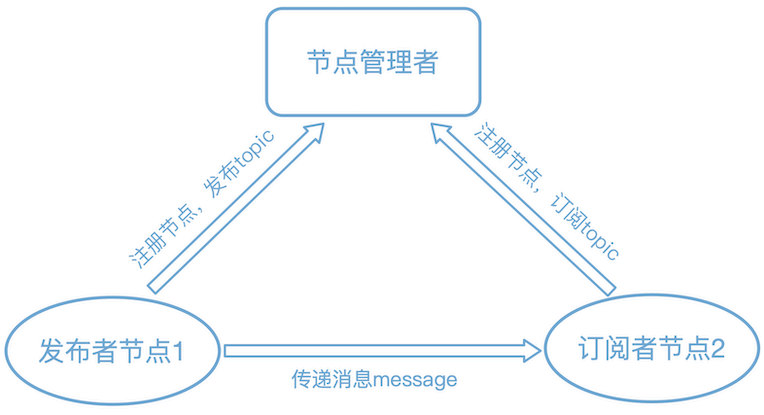
\includegraphics[scale=0.80]{Fig/rossystem.png}
    \caption{\label{frossystem}ROS系统组件图}
\end{figure}

在用户侧,ROS提供了一套机器人导航框架如图\ref{fROSNavstack}所示。该框架接收其它组件提供的地图、传感器信息、定位坐标关联、里程计信息,根据用户指定的导航目标点发布机器人执行的速度指令以运动到目标点。具体来说,ROS使用SLAM算法,通过获取传感器数据(如激光雷达或摄像头数据)和机器人运动信息来实时构建环境地图,然后,在创建的二维栅格地图的基础上,通过自适应蒙特卡洛(Adaptive Monte Carlo Localization, AMCL)等定位算法和传感器数据来实时估计机器人的位姿,最后,提供了move\_base作为导航框架主体,由局部、全局代价地图、全局规划期、局部规划期、失败恢复行为等组件来执行导航任务。

\begin{figure}[htbp]
    \centering
    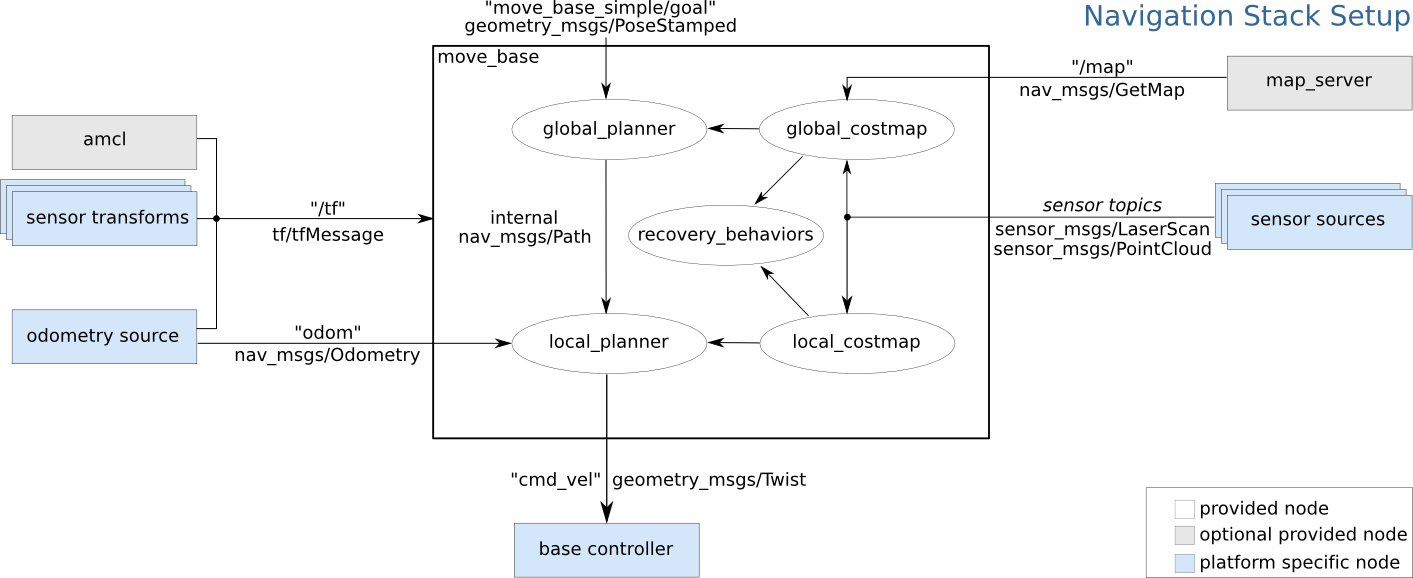
\includegraphics[scale=0.50]{Fig/ROSNavstack.png}
    \caption{\label{fROSNavstack}ROS导航框架图}
\end{figure}


除了上述的核心功能以外,ROS还提供了丰富的工具和生态系统,如可以实时显示机器人传感器数据、地图、路径等信息的可视化工具RViz、允许开发者在虚拟环境中测试机器人算法的高保真物理仿真环境Gazebo、用于记录机器人运行时的传感器数据工具ROS Bag,来帮助开发者更高效地开发和调试机器人系统。本文采用ROS系统的通信机制、导航方法和仿真环境来实现目标物体导航。


\section{联合标定}
激光雷达和单目相机在移动机器人上有着各自的坐标系,为了让激光雷达感知到的物体和单目相机认知到的物体能够对应起来,需要对它们进行联合标定工作。这里使用张正友标定法\cite{zhang2002flexible}进行联合标定,具体的过程如下图\ref{Calibration}所示。图中存在三个坐标系,分别是以标定板左下角为原点的世界坐标系${\rm{Poin}}{{\rm{t}}_W} = {[{X_W},{Y_W},{Z_W}]^T}$,以单目相机为原点的相机坐标系${\rm{Poin}}{{\rm{t}}_C} = {[{X_C},{Y_C},{Z_C}]^T}$和以激光雷达为原点的激光雷达坐标系${\rm{Poin}}{{\rm{t}}_L} = {[{X_L},{Y_L},{Z_L}]^T}$。
\begin{figure}[htbp]
    \centering
    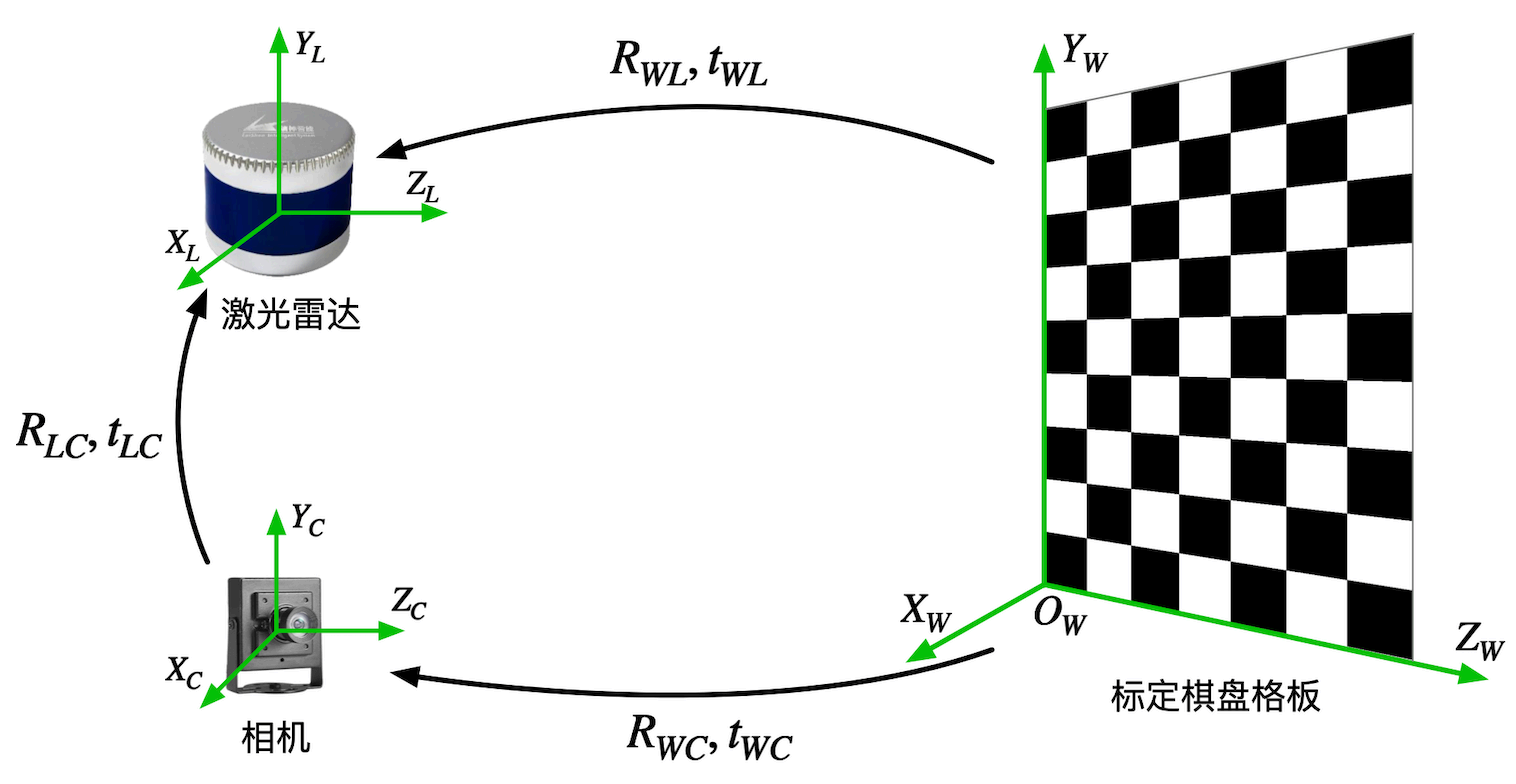
\includegraphics[scale=0.50]{Fig/joinCalibration.png}
    \caption{\label{Calibration}激光雷达和单目相机联合标定}
\end{figure}

联合标定的目的就是要找到相机坐标系和激光雷达坐标系之间的旋转矩阵和平移矩阵,即图中的${\rm{R}}_{LC}$和${\rm{t}}_{LC}$,使得激光雷达的点云能够映射到图像之中,将雷达感知到的物体与相机认知识别到的物体 对应起来。为此需要借助棋盘格标定板来求解它们直接的变换关系矩阵。

首先,相机坐标系中的三维坐标点${\rm{Poin}}{{\rm{t}}_C}$与像素平面上的二维坐标点${P_{uv}}$之间的转换关系可以表示为:
\begin{equation}
Z{P_{uv}} = Z\left[ {\begin{array}{*{20}{c}}
u\\
v\\
1
\end{array}} \right] = K\left[ {\begin{array}{*{20}{c}}
{{x_C}}\\
{{y_C}}\\
{{z_C}}
\end{array}} \right] = K \cdot {\rm{poin}}{{\rm{t}}_C}
    \label{myeq1}
\end{equation}

然后,在激光雷达坐标系下空间的任意一点都可以通过旋转矩阵${\rm{R}}_{LC}$和平移矩阵${\rm{t}}_{LC}$在另一坐标系中进行表示,它们之间的转换关系可以表示为:
\begin{equation}
{\rm{Poin}}{{\rm{t}}_C} = \left[ {\begin{array}{*{20}{c}}
{{x_C}}\\
{{y_C}}\\
{{z_C}}
\end{array}} \right] = {{\rm{R}}_{LC}} \cdot \left[ {\begin{array}{*{20}{c}}
{{x_L}}\\
{{y_L}}\\
{{z_L}}
\end{array}} \right] + {{\rm{t}}_{LC}} = {{\rm{R}}_{LC}} \cdot {\rm{Poin}}{{\rm{t}}_L} + {{\rm{t}}_{LC}} 
    \label{myeq2}
\end{equation}
将上式左项移动到右侧,变形可得:
\begin{equation}
    \delta \left( {{R_{LC}},{t_{LC}},{\rm{poin}}{{\rm{t}}_C},{\rm{poin}}{{\rm{t}}_L}} \right) = {R_{LC}} \cdot {\rm{poin}}{{\rm{t}}_C} + {t_{LC}} - {\rm{poin}}{{\rm{t}}_L}
    \label{myeq3}
\end{equation}

因此,借助棋盘格标定板找到多组相机坐标系和激光雷达坐标系下对应的点,使得上式中的$\delta \left( {{R_{LC}},{t_{LC}},{\rm{poin}}{{\rm{t}}_C},{\rm{poin}}{{\rm{t}}_L}} \right)$取得最小,即可得到旋转矩阵${\rm{R}}_{LC}$和平移矩阵${\rm{t}}_{LC}$,即:
\begin{equation}
    \left( {{R_{LC}},{t_{LC}}} \right) = \mathop {\arg \min }\limits_{{R_{LC}},{t_{LC}}} \frac{1}{2}{\sum {\left\| {\delta \left( {{R_{LC}},{t_{LC}},{\rm{poin}}{{\rm{t}}_C},{\rm{poin}}{{\rm{t}}_L}} \right)} \right\|} ^2}.
    \label{myeq4}
\end{equation}
上述非线性最小二乘方程可以使用Levenberg-Marquadt算法\cite{more1977levenberg}将其化成线性方程进行求解,且具有较快的收敛速度。获得的旋转平移矩阵将用于后续第四章的局部路径部分。



\section{目标检测网络}
在目标物体导航任务中,部署模型的智能体通过目标检测网络对视觉观测进行编码,以提取周围环境的局部特征,即识别环境中的物体语义信息及其空间位置。这些关键信息用于精准定位感兴趣的目标,并辅助智能体确定导航方向、规划通向目标的最优路径,同时在行进过程中有效规避障碍物。

目标检测是计算机视觉领域的一项基础性任务,其目标是从图像或视频中定位并识别出感兴趣的目标物体。与图像分类任务不同,目标检测不仅需要识别出图像中存在的物体类别,还需要精确地用锚框(Anchor)的形式定位出每个物体的位置信息及其对应的置信度分数。在深度学习兴起之前,目标检测主要依赖于手工设计的特征提取方法和机器学习分类器\cite{viola2001rapid}。但这类传统方法存在特征设计复杂、泛化能力有限等问题,难以应对复杂场景下的目标检测任务。

随着深度学习技术的快速发展,特别是卷积神经网络(Convolutional Neural Network,CNN)\cite{taye2023theoretical}在图像分类的任务中取得的巨大成功,目标检测领域也迎来了革命性的突破。目前,目标检测可以分为两大类别:单阶段 (One-stage)检测算法和两阶段(Two-stage)检测算法。前者将目标检测任务视为一个统一的回归问题,一次性直接在图像上进行目标分类和锚框预测而不需要额外的区域提案生成步骤。因此这种方法通常具有较快的推理速度,适用于实时目标检测的场景,但在跟踪小物体或密集目标时效果较差。经典的One-stage目标检测模型包括:
\begin{enumerate}[topsep = 0 pt, itemsep= 0 pt, parsep=0pt, partopsep=0pt, leftmargin=44pt, itemindent=0pt, labelsep=6pt, label=(\arabic*)]
    \item 	YOLO\cite{redmon2016you}:早期YOLO系列的算法采用网格划分策略,它将输入图像分割成等尺寸的单元,让每个单元同时预测若干预设锚框的空间坐标、类别概率及置信度分数。在生成密集预测结果后,系统再通过非极大值抑制技术筛选最优边界框以去除冗余检测。这类方法的显著特点是检测效率高。得益于其单阶段检测架构,它无需区域建议等预处理步骤即可完成目标识别。然而,YOLO过于依赖非极大值抑制进行后处理以得到正确的检测框,这阻碍了其的端到端部署,并且对推理延迟产生了不利影响。除此之外,YOLO的各种组件设计缺乏全面深入的检查,导致明显的计算冗余,限制了模型的能力。与两阶段的目标检测算法相比,在面对小尺度目标或背景复杂的图像时YOLO的检测精度存在一定局限。
    \item	SSD\cite{liu2016ssd}:SSD使用预训练的卷积神经网络在特征提取网络的不同层次获取多个尺度的特征图,这些特征图分别用于检测不同大小的目标。但这种方法需要人工设置预测边框的初始尺度和长宽比的值而不能直接通过学习获得,这导致调试过程十分依赖经验,并且对小尺寸的目标识别效果仍然较差,存在特征提取不充分的情况。
\end{enumerate}

Two-stage目标检测算法则将目标检测任务分为两个阶段。首先利用区域提案网络(RPN)生成一组候选目标区域,然后对每个候选区域进行分类和边界框回归。Two-stage算法通常在准确性上表现更好,尤其擅长处理小目标和复杂场景,但相对于One-stage算法,可能需要更多的计算资源和
时间。代表性的Two-stage目标检测模型包括:
\begin{enumerate}[topsep = 0 pt, itemsep= 0 pt, parsep=0pt, partopsep=0pt, leftmargin=44pt, itemindent=0pt, labelsep=6pt, label=(\arabic*)]
    \item 	RCNN系列:包括RCNN\cite{girshick2014rich}、fastRCNN\cite{girshick2015fast}、FasterRCNN\cite{ren2016faster}等。这类算法首先通过候选框生成网络(Region Proposals Network, RPN)来生成一系列可能包含目标的候选框,然后针对每个候选区域都会通过一个预训练的卷积神经网络中提取特征或者对每个候选区域使用RoI、cite{doukas2007region}池化,将每个候选区域都提取并缩放至固定大小的特征,最后使用全连接层进行目标分类和边界框回归。但这类检测方法的实时性不足。
    \item	基于Transformer:DETR\cite{carion2020end}是Transformer目标检测算法的开篇之作。它通过引入Transformer架构将目标检测过程视为一个由图形到集合的预测问题,消除了如锚框生成和非极大值抑制等后处理过程,通过二分匹配和一个转换器、编码器、解码器的结构和端到端的方式来进行目标的预测和类别的区分。但这类方法的训练时间长,模型的收敛速度慢,且在小物体的检测时性能较差。
\end{enumerate}

\begin{figure}[htbp]
    \centering
    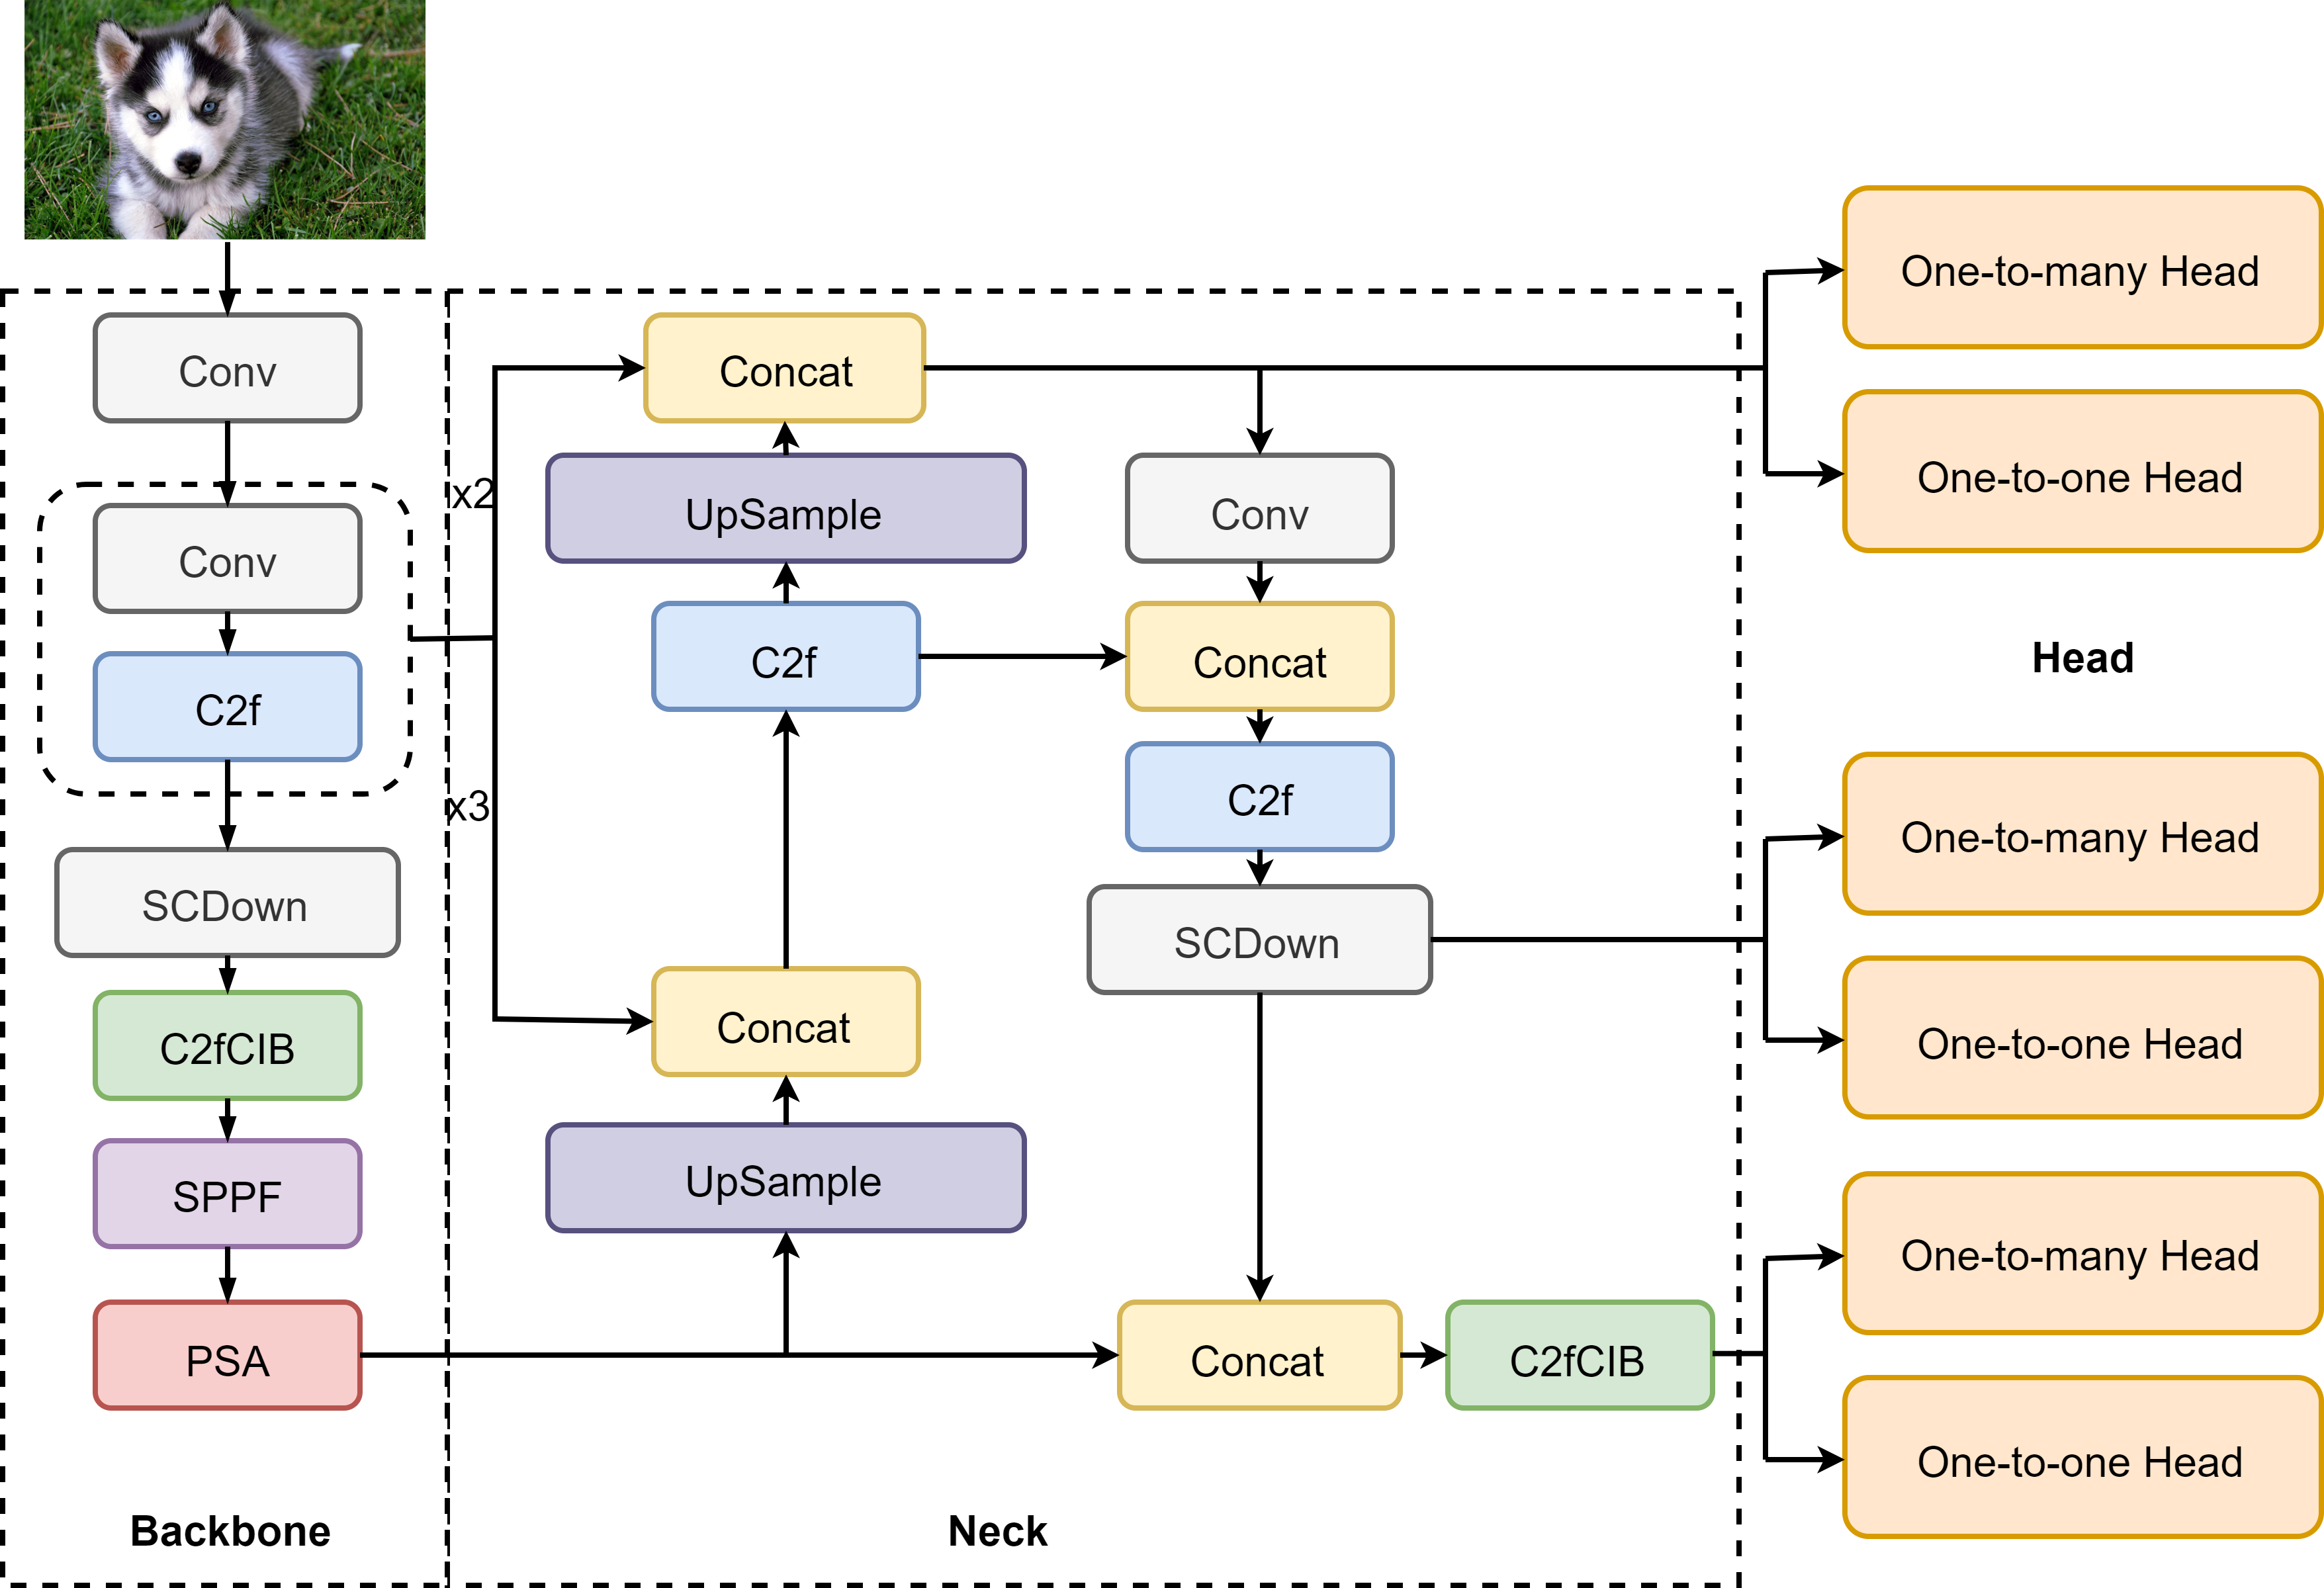
\includegraphics[scale=0.12]{Fig/yolonet.png}
    \caption{\label{fyolonet}YOLOV10网络}
\end{figure}

为了满足整个导航过程中目标检查所需的实时性和可靠性,本文使用的目标检测网络是YOLOV10网络\cite{wang2025yolov10},如图\ref{fyolonet}所示。YOLOV10与YOLOV8\cite{varghese2024yolov8}相比在整体的网络结构上基本保持一致,网络分为骨干网络(Backbone)、颈部(Neck)、头部(Head)三个部分。首先将图片输入骨干网络中提取图像的全局和局部特征,在颈部通过Upsampling、Concat和注意力机制卷积网络增强特征的表达能力,实现有效的特征提取和融合,并在头部将颈部提取的特征映射到最终的输出空间,生成网络的最终预测结果。然而,相较于后者,YOLOV10为了实现更加轻量化的端到端部署而做出了几点重要的优化:
\begin{enumerate}[topsep = 0 pt, itemsep= 0 pt, parsep=0pt, partopsep=0pt, leftmargin=44pt, itemindent=0pt, labelsep=6pt, label=(\arabic*)]
    \item 	轻量化分类头(Lightweight Classification Head):在YOLOV8网络结构中Head部分的分类头的参数量和计算量比回归头更大,但后者对检测精度的影响更大,因此减少分类头的卷积参数量以达到轻量化模型的目的。
    \item	空间-通道分离下采样(Spatial-Channel decoupled downsampling, SCDown):YOLOV8使用一个标准卷积时实现空间下采样和通道变换,SCDown将这两种操作进行解耦,先通过逐点卷积调节通道维度,然后通过深度卷积进行空间下采样,保证降低计算成本的同时最大限度保留信息。
    \item   精度驱动的模型设计:在小模型规模的深层阶段使用大核卷积(Large-kernel Conv)来扩大感受野,增强模型能力;针对计算开销过大的自注意力机制设计了一种高效的部分自注意力(Partial self-attention, PSA),对分辨率最低的特征的一半进行计算,将对于全局的学习能力以较小的计算成本融入到网络中。通过这些方法可以在不显著增加计算成本的情况下提升模型的性能。
    \item   基于秩的块设计:提出了一种紧凑的倒置块(CIB)结构,它采用廉价的深度卷积进行空间混合,通过成本效益高的点卷积进行通道混合,解决了简单地为所有阶段应用相同的块设计导致计算冗余的问题。
\end{enumerate}


\section{多模态特征融合网络}

多模态特征融合是指整合多种来源或形式的数据信息,通过协同作用提升系统的认知能力或执行效果。这种技术旨在充分发挥各模态间的优势互补特性,从而优化系统在诸如模式辨识、类别划分以及内容生成等任务中的综合表现。

在后续的目标物体导航过程中,将利用多模态特征提取网络来融合词嵌入网络的目标特征、目标检测网络编码的局部特征和卷积神经网络编码的全局特征,以得到可以指导机器人进行导航的动作决策。现阶段不同的多模态融合方法按照融合的阶段可以分为以下三种类型:
\begin{enumerate}[topsep = 0 pt, itemsep= 0 pt, parsep=0pt, partopsep=0pt, leftmargin=44pt, itemindent=0pt, labelsep=6pt, label=(\arabic*)]
    \item 	特征级融合:这种融合方法是在神经网络的核心处理模块之前,通常是在数据输入环节,将多种模态的特征进行整合。比如,在数据输入阶段就将视觉信息和文本信息进行融合。
    \item	模型级融合:这种融合方式选择在神经网络的中间层级进行多模态信息的整合。具体做法可以是将各模态经过独立学习后的特征表示进行合并,然后再进行后续的网络处理。
    \item	决策级融合:该策略在完成各模态的独立处理后进行融合,整合过程发生在决策或输出层。在每个模态的数据都经过单独处理后,最终将各模态的输出结果进行综合以形成最终决策。这种方法的优势在于其灵活性,能够兼容经过预训练的单模态模型。
\end{enumerate}

本文将采用第三种融合方法,即使用Transformer网络进行后期的决策级融合,Transformer网络的操作流程如图\ref{ftransformer}所示。Transformer网络的核心创新在于采用了多头自注意力机制\cite{niu2021review}。自注意力的核心原理是通过计算序列中各元素间的关联度,生成相应的注意力权重,并基于这些权重对序列元素进行加权整合。多头机制则通过并行使用多个注意力单元,使每个单元能够学习到不同的权重分布,从而让模型能够在多个特征子空间中对输入序列进行多样化表征。这种设计使Transformer能够突破传统模型的局部窗口限制,实现对序列全局信息的有效捕捉。多个注意力单元可以分别聚焦于不同类型的信息特征,显著增强了网络在处理多模态数据时的特征融合能力。具体来说:
\begin{equation}
    \begin{array}{c}
Attention\left( {Q,K,V} \right) = softmax\left( {\frac{{Q{K^T}}}{{\sqrt {{d_k}} }}} \right)V\\
hea{d_i} = Attention\left( {QW_i^Q,KW_i^K,VW_i^V} \right)\\
MultiHead\left( {Q,K,V} \right) = Concat\left( {hea{d_1}, \ldots ,hea{d_n}} \right){W^O}
\end{array}
    \label{myeq7}
\end{equation}
其中,查询($Q$)、键($K$)和值($V$)由输入序列通过三个线性变换获得的矩阵,$W_i^Q$、$W_i^K$和$W_i^V$分别是$Q$、$K$和$V$的权重矩阵,${d_k}$表示特征维度,$hea{d_i}$表示第i个注意力头,${W^O}$表示连接多个注意力头输出的权重矩阵Attention表示子注意力机制,MultiHead是多头自注意力机制。
\begin{figure}[htbp]
    \centering
    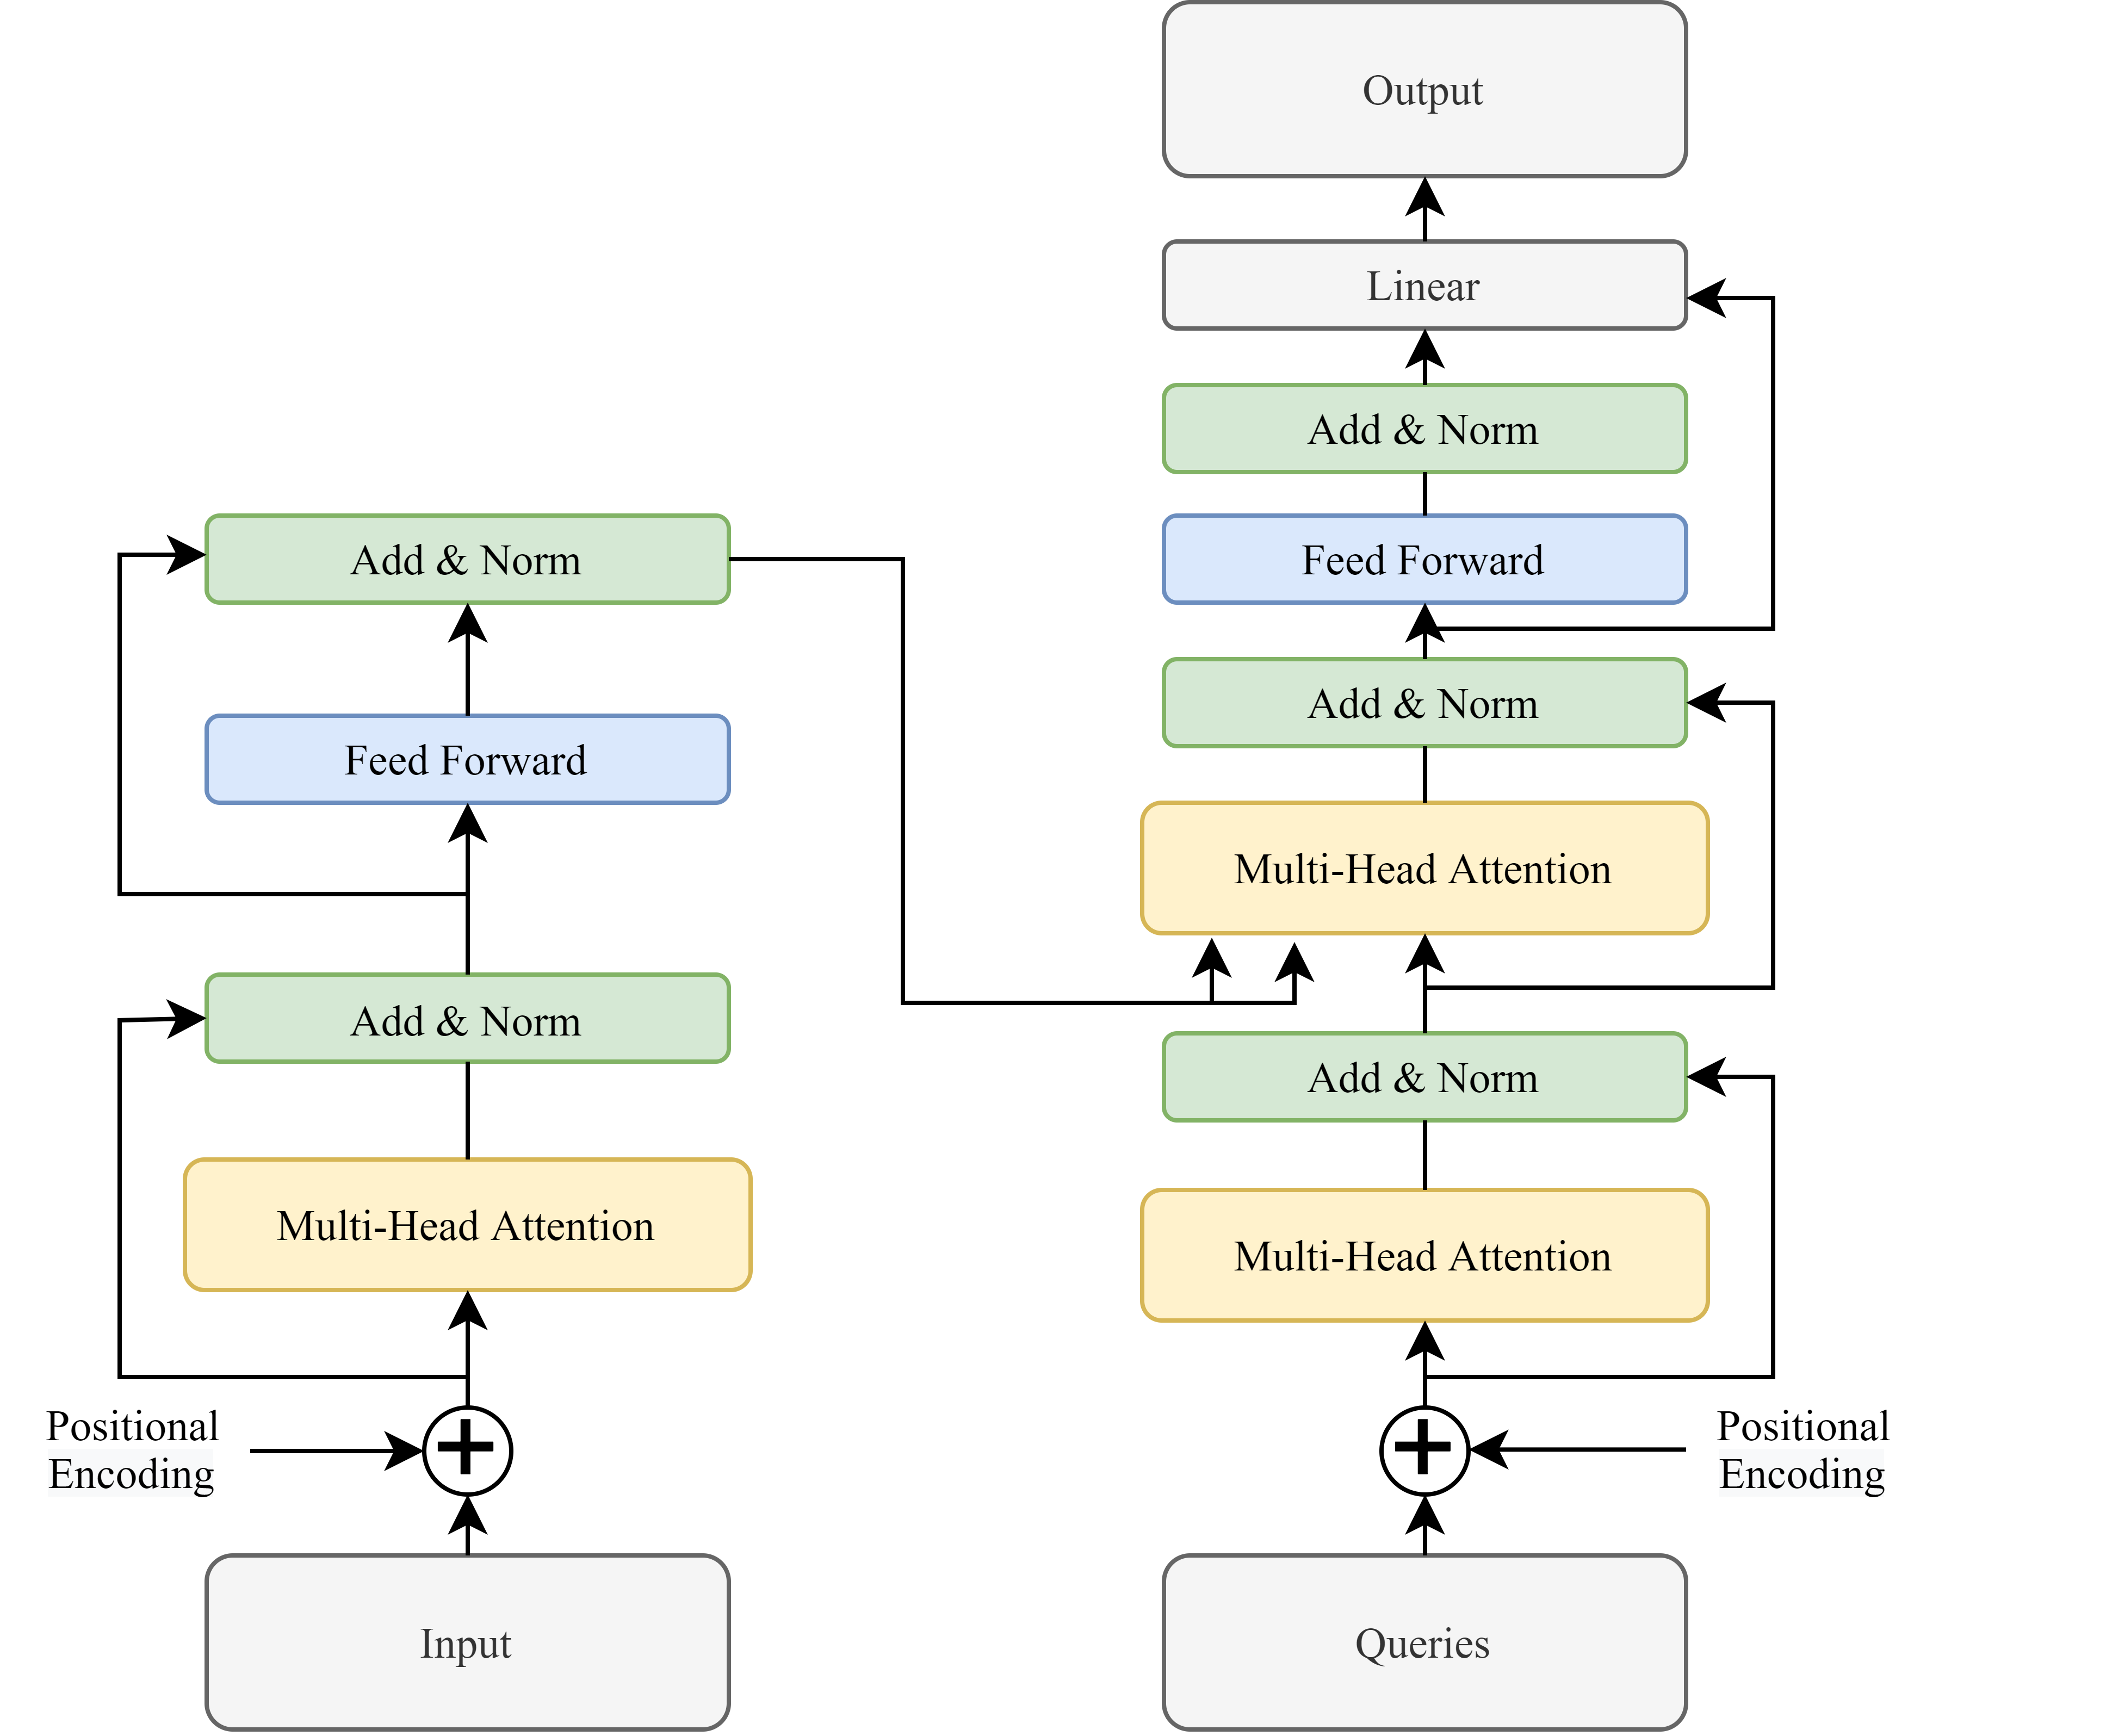
\includegraphics[scale=0.10]{Fig/transformer.png}
    \caption{\label{ftransformer}Transformer网络结构}
\end{figure}

\section{点云聚类}
三维激光雷达所获取得点云信息在空间中是由一堆离散的点进行表示的,如何区分每个点属于哪个物体是聚类算法需要解决的问题。点云通常利用其特征属性进行聚类,对每个点空间或局部空间进行特征的提取或者转换以得到多种属性,如法向量、密度、距离、强度等,将不同属性的点云分割开来\cite{himmelsbach2010fast}。常见的点云处理方法有欧式聚类、密度聚类、超体聚类等,针对不同的场景各个算法在耗时和准确率方面各有优势。在目标物体导航的过程中要求系统需要更强的实时性,因此本文采用欧式聚类\cite{liu2021point}方法对三维点云进行预处理。

欧式聚类法在点云密集的情况下需要进行额外的优化以保证其实时性,这里采用点云栅格化和kd树对算法进行加速优化\cite{guo2023kd}。栅格化方法首先将扫描区域划分为若干网格单元,将三维点云投影至二维平面,保持z轴数值不变的同时,将每个网格内点的x、y坐标统一为该网格中心点坐标。随后进行去重处理,对于x、y坐标相同且z值相近的点只保留一个代表性点,通过栅格化方法对点云数据进行处理能够显著减少计算复杂度。除此之外,本文利用PCL库中的KdTree->setInputCloud()函数将栅格化后的点云构建为k维二叉树结构,借助kd树结构优化近邻搜索过程,进一步提升欧式聚类算法的效率。

距离阈值是用来区分不同簇点云的重要参数,当一个点集${P_m} = \left\{ {{p_m} \in P} \right\}$与另一个点集${P_n} = \left\{ {{p_n} \in P} \right\}$之间的最小距离大于给定的距离阈值${d_{th}}$,则可以认为这两个点集为两簇不同的点集。因此,点云簇为两簇不同的点云的条件可以表示为
\begin{equation}
    \min \left\| {{p_m} - {p_n}} \right\| \ge {d_{th}}
    \label{myeq5}
\end{equation}

激光雷达所产生的点云具有发散的特点,即随着与原点的距离的增加,点云的密度会逐渐下降。如图\ref{fcarpoints}所示,随着车辆与激光雷达之间的距离增大,其反射生成的点云分布密度显著降低。传统的欧式聚类算法依赖于固定的距离阈值来划分障碍物,这种方法难以应对点云密度随距离变化的情况。针对这种发散的特性,文本根据距离激光原点的远近程度设计了一种改进的欧式聚类方法,如\eqref{myeq6}所示,当点云离原点距离越远时所采用的距离阈值参数也越大。
\begin{figure}[htbp]
    \centering
    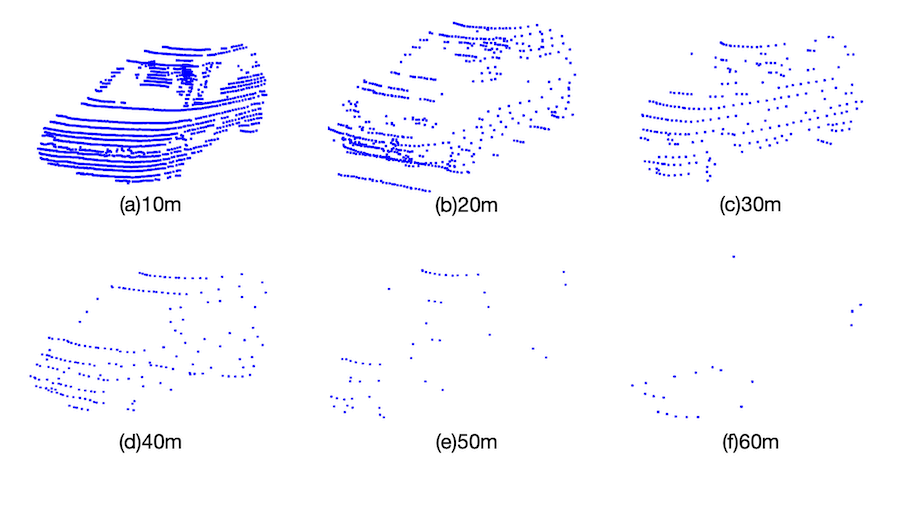
\includegraphics[scale=0.75]{Fig/carpoints.png}
    \caption{\label{fcarpoints}障碍物点云随着距离增加变稀疏}
\end{figure}
\begin{equation}
    {d_{th}} = \left\{ {\begin{array}{*{20}{c}}
{5cm}\\
{10cm}\\
{15cm}\\
{20cm}
\end{array}} \right.{\rm{ }}\begin{array}{*{20}{l}}
{0 < Range \le 1.5m}\\
{1.5m < Range \le 3.0m}\\
{3.0 < Range \le 5m}\\
{5m < Range}
\end{array}
    \label{myeq6}
\end{equation}
文本所采用的是16线激光雷达,在离目标距离超过5米时竖直方向上的点过于稀疏,导致目标物体检测的效果不理想,因此超过5米范围的距离阈值则不再进行更新。本文改进的欧式聚类算法的伪代码见Algorithm\ref{algorithm1}。
\begin{algorithm}[!h]
    \caption{可变距离阈值的欧式聚类算法}
    \label{algorithm1}
    \renewcommand{\algorithmicrequire}{\textbf{Input:}}
    \renewcommand{\algorithmicensure}{\textbf{Output:}}
    \renewcommand{\algorithmiccomment}[1]{\hfill $\triangleright$ #1}
    \begin{algorithmic}[1]
        \REQUIRE 激光点云$P$  %%input
        \ENSURE 点云蔟集合$C$    %%output
        \STATE  Grid Downsample and create KD-tree for $P$;
        \COMMENT{对点云进行栅格化和kd树预处理}
        \STATE  create cluster list $C$
        \STATE  create cluster $c$
        \FOR{${p_i} \in P$}
            \STATE  que.push(${p_i}$)
            \COMMENT{遍历点云$P$中的每个点,并将当前点${p_i}$加入队列}
            \WHILE{!que.empty()}
                \STATE  ThresholdGet(${p_i}$)$ \to {d_{th}}$
                \COMMENT{计算当前点对应的距离阈值}
                \STATE  KdtreeSearch($P$,${p_i}$,${d_{th}}$)$ \to P_i^k$
                \COMMENT{使用kd树寻找${p_i}$的邻近点}
                \FOR{${p_j} \in P_i^k$}
                    \STATE  que.push(${p_j}$)
                    \COMMENT{遍历${p_i}$的临近点,并将其加入队列中}
                \ENDFOR
                \STATE  $c = c \cup {p_i}$
                \COMMENT{将找到的这簇点云加入结果集中}
                \STATE  que.pop()
            \ENDWHILE
            $c = \emptyset $
        \ENDFOR
    \end{algorithmic}
\end{algorithm}

点云聚类算法的结果用于后文第四章所介绍的点云映射中,将点云感知信息与图像认知信息的结果相融合,以获得目标检测算法认知到的目标物体的精确位置信息。


\section{本章小结}
本章主要内容是目标物体导航过程中涉及到的一些常用的算法原理和关键技术,主要介绍了ROS系统及传感器间的通讯方法、联合标定、目标检测网络、多模态特征融合网络、点云聚类算法。

%第二章
	
\chapter{全局路径规划导航方法}
为实现移动机器人既能根据自然语言指令中的目标进行导航,又能完成导航至目标半米内的任务,本文提出了一种语言视觉激光多模态融合的机器人导航(Language Vision Lidar Navigation, LVL-Nav)方法。为了能够完成上述任务,我们提出的LVL-Nav将导航任务拆分为已知环境中下的全局路径规划导航和未知环境下的局部路径规划两个部分。本章将详细介绍LVL-Nav方法中的全局路径规划导航方法。主要有目标物体导航任务定义,然后描述了所提出的全局路径规划导航方法的框架设计,最后分别描述了框架中的指令语义提取模块、多模态融合网络模块、方位优化算法和导航点规划算法四个部分。其中指令语义提取模块将非结构化的语言指令通过大语言模型映射到具体的目标空间和方位空间,前者作为多模态融合网络模块中的目标特征与图像编码器和深度图编码器所提取环境的图像特征、深度特征拼接得到的环境特征进行跨模态融合,帮助智能体理解多种模态之间的关系;后者则通过方位优化算法辅助筛选掉冗余的导航点,最后再通过导航点规划在最大化目标与导航点的匹配程度的同时最大化导航成功率。

\section{导航任务定义}
多模态融合的目标物体导航任务要求代理从室内环境中的随机起始位置根据自然语言指令导航到用户依次指定的物体类别,如打印机、餐桌、储物柜等,并且代理被允许使用以第一视角的视觉观察(通常为RGB图像)和激光雷达,其问题可以定义如下:给定自然语言指令$I$和智能体在环境中的初始位姿$S$,通过解析指令要求,在建好的栅格地图中的导航点集中依次推理选择与指令目标序列$\left\{ {{l_i}} \right\}$相匹配的导航点序列$\left\{ {{v_i}} \right\}$,并最终在目标位置的半米内停下以完成导航任务。

一次完整的目标物体导航过程如图\ref{simularity_world}所示,代理在t=0的初始时刻被初始化在房间右上角餐桌附近的$S$点,同时能获得单目相机和激光雷达第一视角的RGB图像和点云数据,以及一条导航指令“Go all the way to the refrigerator, then turn around to the sofa, straight forward past the bed, and stop at the edge of the chair.”。然后智能体根据对指令的理解从当前位置开始执行导航任务,智能体根据推理结果在导航图中的节点之间移动,需要在餐桌附近依次导航到冰箱、沙发、寝室的床和床边的座椅,在经过所有子目标之后在最终目标的位置附近停下。其中,蓝色箭头依次所指的目标是智能体所推理出的所有目标节点。
\begin{figure}[htbp]
    \centering
    \includegraphics[scale=0.05]{Fig/target_nav.png}
    \caption{\label{simularity_world}目标物体导航过程}
\end{figure}



\section{导航框架设计}
目标物体导航是机器人导航中的一个重要子任务和研究方向,其主要目的是通过代理对环境的感知和认知信息依次到达指令给定的目标物体。现有的目标物体导航方法中,
Ke\cite{ke2019tactical}等人提出了一种FAST模型,使用贪婪搜索算法将目标对象描述的编码与动作空间的编码相结合,以导航到下一个目标点。
Hong\cite{hong2020language}等人提出了一种新的语言和视觉实体关系图,通过在语言元素与视觉实体之间传递信息,实现了不同模态之间的高效协同,并将其用于捕捉并模拟文本与视觉之间以及视觉实体之间的相互关系。
Wang\cite{wang2021structured}等人针对代理无法实时捕捉环境布局和进行长期规划这一限制,提出了一种结构化场景记忆(Structured Scene Memory, SSM)导航框架,它可以自适应地捕获和表征环境中的视觉和几何特征以支持当前决策,并模拟迭代算法进行远程推理以实现高效的全局规划,他们的算法在R2R和R4R数据集上的实验结果取得了最优秀的性能。
Pashevich\cite{}等人针对代理无法准确地处理长序列的子任务和理解复杂的人类指令,提出了一种多模态转换器(Episodic Transformer, E.T.),利用合成指令作为中间表示,将理解环境的视觉特征与复杂多样的自然语言指令解耦。
Shah\cite{shah2021ving}等人提出的视觉语言导航方法使机器人能够根据目标图像和环境拓扑图进行导航。
Huang\cite{huang2023visual}等人创新性地提出了一种基于空间映射表示的方法VLMaps,它直接将预训练的视觉语言特征与物理世界的3D重建融合在一起,通过大语言模型可以将自然语言命令转换为一系列可以定位在地图中的开放词汇导航目标,并且允许在多个机器人之间共享以动态生成新的障碍地图。
王湉\cite{王湉2024基于大语言模型的人机交互移动检测机器人导航方法}等人通过场景语义分割和三维重建的方法构建语义地图,再利用语言模型理解并执行指令。

这些目标物体导航方法如图\ref{preview_problem}所示,他们大都强调在环境中提取物体语义、位置、物体关系等丰富的视觉特征表示,并将其与栅格地图中的导航点相关联,以此来告诉代理应该导航到哪个导航点,但这种做法过于关注环境中存在什么物体,缺失了已知环境的拓扑信息,没有利用语义中的方位信息进行导航点的筛选,且视觉语言模型在光线条件变化大的室内的鲁棒性较低,从而导致了导航成功率和导航效率低的问题。
\begin{figure}[htbp]
    \centering
    \includegraphics[scale=0.07]{Fig/pre_problem.png}
    \caption{\label{preview_problem}之前工作存在的问题}
\end{figure}

因此,如何在进行图像观察中的物体语义、位置、物体关系等目标物体视觉表示和栅格地图中所标记导航点的匹配过程中,利用环境中不同导航节点和机器人当前位姿所构成的拓扑信息来辅助代理进行更精确地匹配,优化传统的视觉语言模型以克服其在曝光或欠爆环境下模型性能差的问题,再通过从语言指令中提取的方位信息进行方位优化以筛选掉不在目标方向上的冗余导航点,从而提高指导代理依次导航到目标点的导航成功率和导航效率。

在全局路径规划中我们的导航框架如图\ref{global_framework}所示。$添加流程图及其相应的解释$全局路径规划主要由四个关键模块算法构成。首先,输入的导航指令在经过大语言模型处理之后得到目标序列和动作序列,前者与环境中存在的多个可能的导航点图像一同作为多模态融合网络的输入得到导航点匹配特征,后者在经过方位优化算法后筛选掉冗余的导航点,再基于栅格地图和初始位姿计算获得环境的拓扑图以补足环境拓扑特征,最后通过导航点规划算法综合考虑多种导航策略以获得最终的导航点序列,依次发布导航点以完成导航任务。

我们的方法考虑了之前工作中不足的地方并加以改进。具体来说,视觉图像导航方法的效果在很大程度上取决于多模态融合网络的性能,多模态融合网络通过引入深度信息,优化传统视觉语言模型,提高模型在光线条件变化大的室内的鲁棒性,此外,本文针对室内环境存在多种相同目标的情况,提出了一种方位优化方法,结合指令中提供的方位信息与移动机器人的实时位姿,筛选不符合方位条件的冗余导航点,进一步提高全局路径规划中导航点与目标匹配的正确率,最后通过环构建的环境拓扑图结合上述两个算法结果进行导航点规划算法,最终获得导航点序列以执行全局路径导航。
\begin{figure}[htbp]
    \centering
    \includegraphics[scale=0.09]{Fig/global_framework.png}
    \caption{\label{global_framework}全局路径规划导航框架}
\end{figure}


\section{指令语义提取模块}
房间到房间(Room-to-Room,R2R)是一个用于验证视觉语言导航(VLN)模型的基准数据集\cite{anderson2018vision}。R2R数据集包括两部分内容:指令和环境,其中环境通过导航图来表示,如图\ref{r2r_nav},而导航图的节点代表了以智能体为中心视野的全景图像位置,节点之间的边则定义了智能体可以到达的邻近位置。在R2R的任务中,智能体会根据自然语言指令进行导航,而视觉图像会随着智能体的移动进行更新。举例来说,给出指令“Turn left and exit the room. Keep walking along the hall past the kitchen area. Wait by the doorway to the dining table area.”后,智能体根据对指令的理解,从起始点开始执行任务。它根据推理的结果在导航图的节点间移动,最终到达目标位置并停止。
\begin{figure}[htbp]
    \centering
    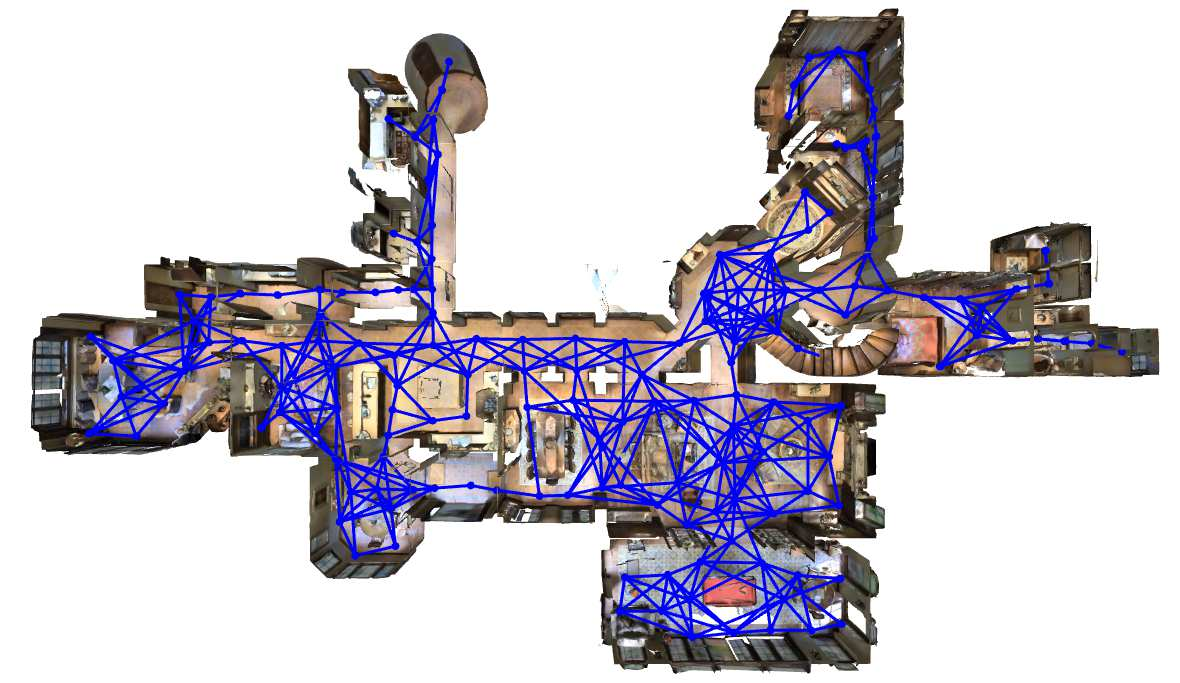
\includegraphics[scale=0.55]{Fig/r2r_nav.png}
    \caption{\label{r2r_nav}R2R数据集中的导航图}
\end{figure}

视觉语言导航技术使人类能够使用自然语言与机器人进行交流,从而使机器人能够基于对场景的感知和对语言指令的理解来执行相应的导航任务。然而,目前大多数关于视觉语言导航的研究仍然面临诸多挑战,其中最突出的问题之一是难以适应人类语言的复杂性和多样性。许多现有方法往往忽视或无法全面提取指令中蕴含的关键信息,例如目标位置和方位描述,这在很大程度上限制了该技术在实际智能制造环境中的广泛应用。通过统计R2R指令集中所存在的所有单词分布得到图\ref{instruction_words}。分析结果表明,通过利用大语言模型,可以更准确地解析指令中的目标和方位信息。此外,基于提取出的方位信息,智能体能够更有效地过滤掉复杂室内环境中由于方向不同而产生的大量错误目标,从而显著提升导航任务的执行精度和鲁棒性。这一能力对于提高视觉语言导航系统的实际应用价值至关重要。
\begin{figure}[htbp]
    \centering
    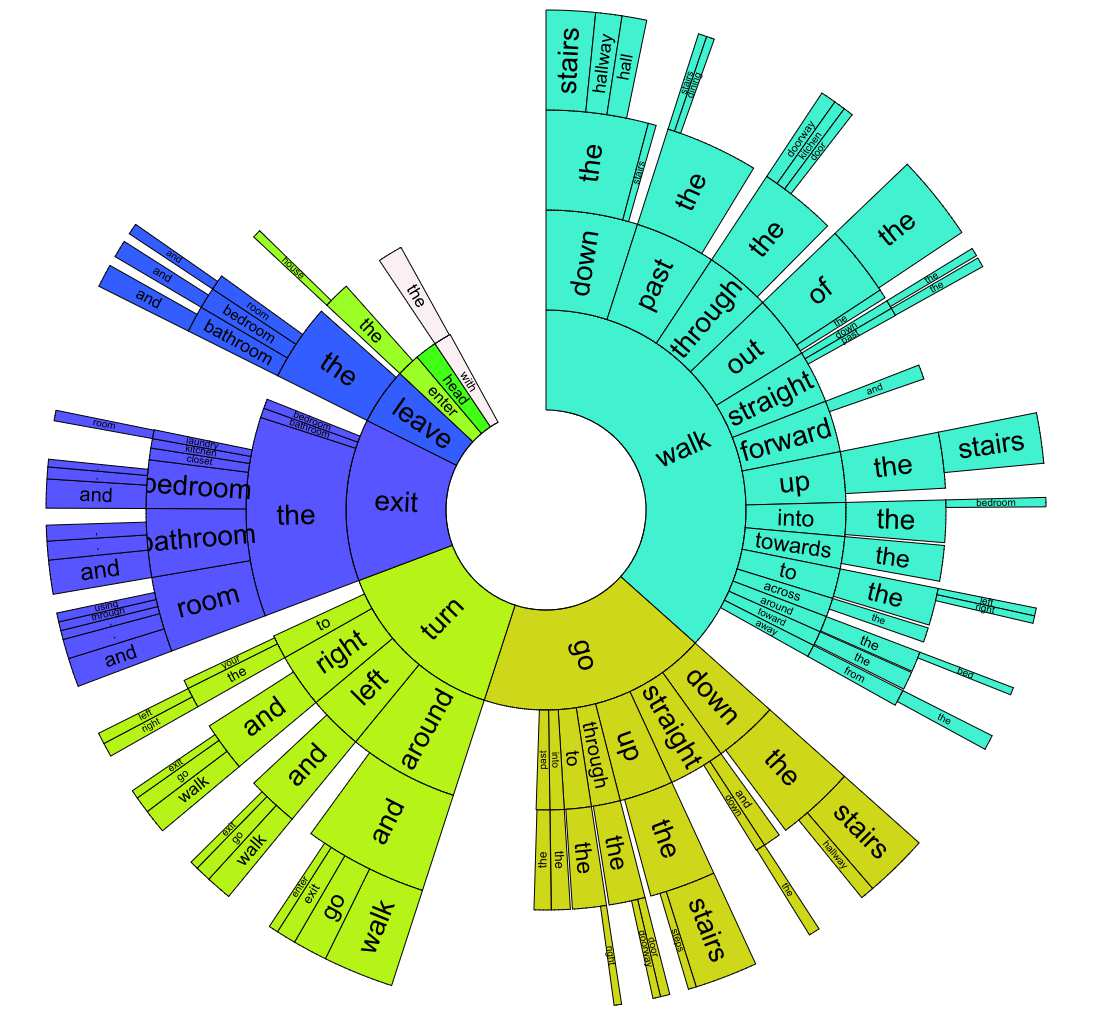
\includegraphics[scale=0.55]{Fig/instruction_words.png}
    \caption{\label{instruction_words}R2R指令集中的方位指示分布}
\end{figure}

本文提出并采用了一种专门设计的任务提示模板,该模板能够高效且准确地引导语言模型,将各种不同形式的导航指令解析并转换为导航任务执行所需的具体目标和方位序列。通过这种方法,我们能够为多模态融合网络以及方位优化提供更加清晰且具体的任务语义信息,从而提升整体导航系统的理解能力和执行效率。在实验的过程中,我们通过输入任意形式的导航指令,选用了Noun Chunks、GPT3.5、GPT4.0和深度求索(DeepSeek)四种不同的语言模型进行自然语言导航指令解析测试,测试结果如表\ref{deepseekcmp}所示。
\begin{table}
\caption{\label{deepseekcmp}不同的语言模型测试结果}
\centering
\small
\begin{tabular}{cccc}
    \hline
    Noun Chunks & GPT3.5 & GPT4.0 & DeepSeek \tabularnewline 
    \hline 
    0.80 & 0.88 & 0.96 & 0.96 \tabularnewline
    \hline 
\end{tabular}
\end{table}
实验结果表明,在我们设计的导航指令提示任务中,Noun Chunks和GPT3.5对复杂句式的处理能力较差,在面对简写、俚语等语言变体导航指令时输出的目标序列和方位序列存在错误、乱序的情况,会影响系统整体导航的成功率。除此之外,虽然GPT4.0在我们设计的任务中取得了较好的结果,但是移动机器人在接收指令后的很长一段时间都在等待模型响应,其缓慢的响应速度会降低系统整体的导航效率。而DeepSeek则通过垂直领域预训练、知识增强和验证机制的技术路线,在保证它本身能准确地完成特定的语言推理任务的同时还能快速高效地进行响应,因此本文选用DeepSeek\cite{guo2025deepseek}作为核心语言模型。

为了确保提取结果的准确性,我们通过详细描述任务内容,并提供正确的目标与方位提取示例,引导模型学习合理的输出模式,使其生成的结果尽可能符合预期要求。具体而言,当输入一条随意表达的导航指令后,该模型会自动分析并提取其中包含的目标与方位信息,并将其转换为标准化的数据格式,方便后续的导航任务执行。实验中,该模型对不同风格的导航指令均表现出较高的适应能力和准确性,其提取结果如图\ref{Extract_orien}所示,进一步证明了该方法在导航任务中的有效性和实用价值。


\begin{figure}[htbp]
    \centering
    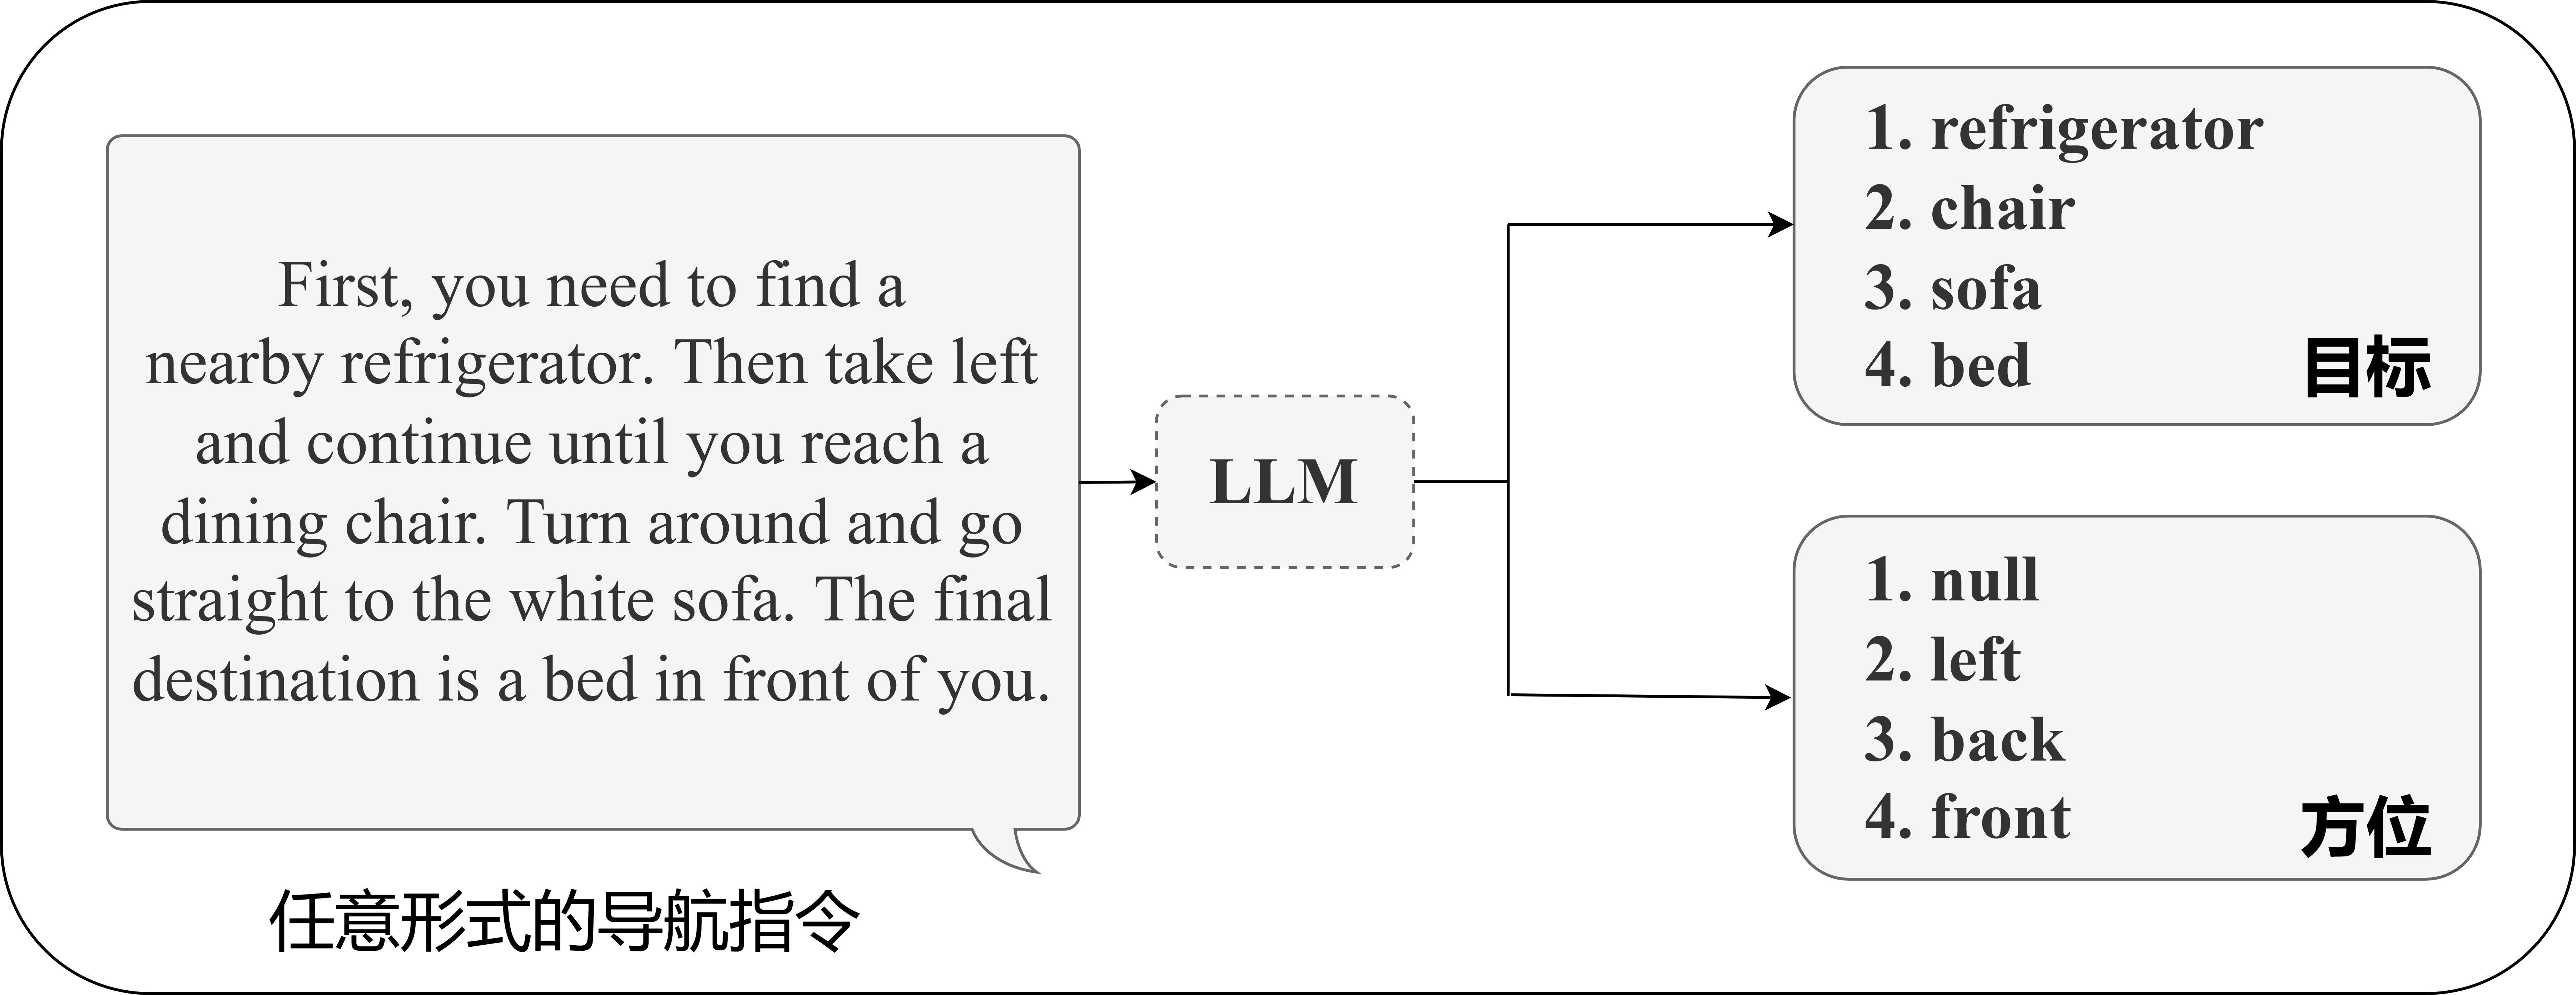
\includegraphics[scale=0.05]{Fig/Extract_orien.png}
    \caption{\label{Extract_orien}指令语义提取模块}
\end{figure}




\section{多模态融合网络模块}
CLIP(Contrastive Language-Image Pre-training)多模态融合网络\cite{radford2021learning}是一种基于对比学习的模型,能够将图像和文本映射到同一个嵌入空间中,从而使得匹配的图像-文本对的特征向量尽可能接近,而不匹配的图像-文本对的特征向量尽可能远离。这种学习策略使得CLIP在没有特定任务训练数据的情况下,依然能够有效地执行分类和搜索任务,展现出极高的泛化能力和适应性。因此,CLIP具有极大的灵活性和通用性,在多模态建模领域得到了广泛关注,并在众多计算机视觉和自然语言处理任务中展现出优越的性能。

在利用视觉语言进行导航的任务中,一个核心挑战是如何高效且准确地将语义目标与环境图像进行匹配,并在此基础上规划出一条符合指令描述的全局导航点序列,以确保导航智能体能够按照预期完成路径规划。InteriorNet\cite{li2018interiornet}是一个大规模、多传感器、照片级真实感的室内场景数据集,由帝国理工学院和KooLab联合创建,该数据集来源于真实的生产制造,包含约100万个家具CAD模型和2200万个室内布局。为了研究CLIP在不同光照环境下的表现,我们随机选取了该数据集中的若干图像,并通过计算直方图的方法将其划分为4个曝光程度不同的子数据集。这4个子数据集分别对应过度欠爆、轻微欠爆、正常曝光、明显过曝的情况。随后使用CLIP模型在这些数据集上进行了图像-文本匹配测试,并评估其匹配的正确率,如表\ref{Matching_accuracy}所示。实验结果表明,在光照条件良好的室内环境下,CLIP能够稳定且可靠地完成图像与文本的匹配任务。然而,当图像出现曝光过度或欠曝的情况时,CLIP的匹配正确率明显下降,表现出较大的不稳定性。这一发现表明,尽管CLIP在标准光照条件下能够提供较为理想的匹配效果,但其在室内的复杂光照环境下仍然存在一定的局限性。

\begin{table}[ht]
	\centering
	\caption{模型进行图像文本匹配的正确率} % 表格标题
	\begin{tabular}{ccccc} % 这里定义了列的格式
	\toprule % 上方的横线
	色阶范围 & [0,60] & [61,120] & [121,180] & [181,255]  \\ % 表头行
	\midrule % 中间的横线
	CLIP & 32.43\% & \textbf{99.12\%} & 89.38\% & 37.72\% \\ % 第一行数据
	CLIDP & \textbf{44.95\%} & 98.23\% & \textbf{92.04\%} & \textbf{42.28\%} \\ % 第二行数据
	\bottomrule % 底部的横线
	\end{tabular}
	\label{Matching_accuracy}
\end{table}

为了解决现有视觉语言导航系统在不同光照条件下匹配能力不稳定的问题,本文针对多模态融合网络的特征提取能力进行了改进,引入了一种深度图像编码器以提取环境中的深度信息从而扩展了模型所能捕捉的特征维度。这种改进能够确保模型在曝光过度或欠曝的复杂光照条件下,仍然可以依赖深度特征信息进行准确的图像-文本匹配,而不仅依赖于颜色或纹理等受光照影响较大的视觉特征。基于这一思路,我们提出了一种新的多模态融合框架CLIDP(Contrastive Language-Image-Depth Pre-training),其整体架构如图\ref{CLIPD_framework}所示。
\begin{figure}[htbp]
    \centering
    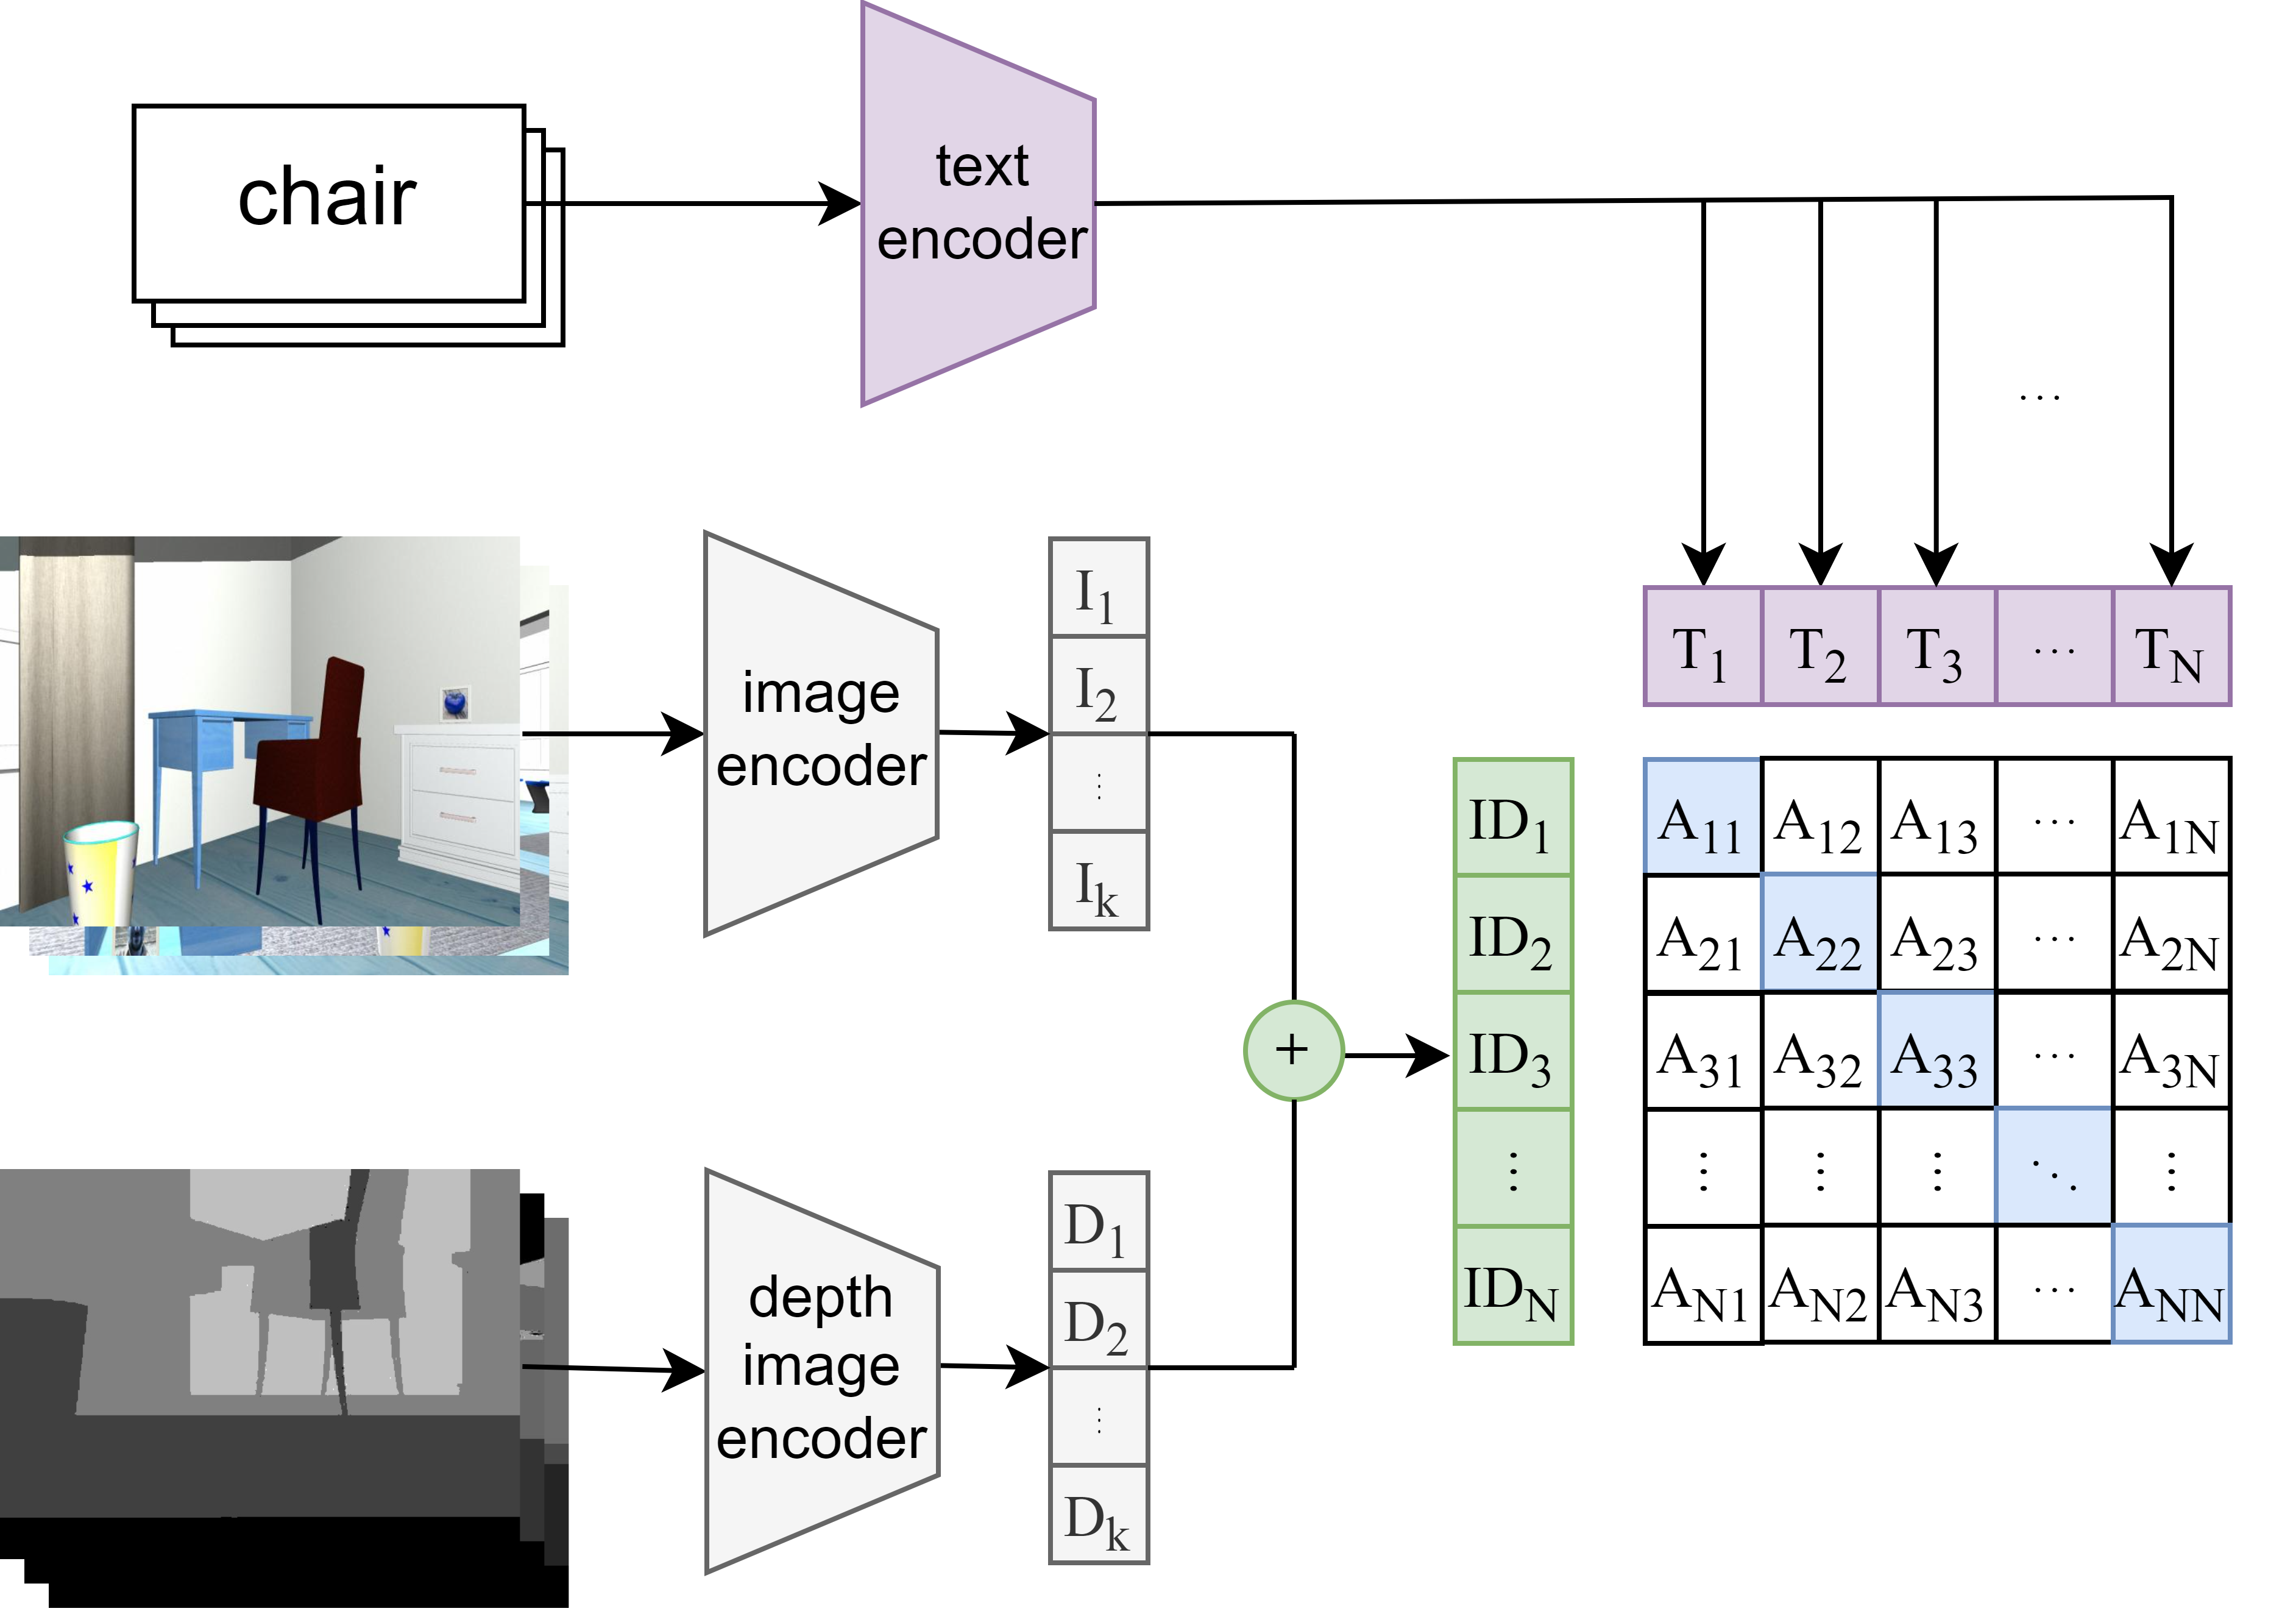
\includegraphics[scale=0.09]{Fig/CLIPD_framework.png}
    \caption{\label{CLIPD_framework}CLIPD多模态融合网络框架}
\end{figure}

CLIDP多模态融合网络在预训练模型ViT-B-32\cite{radford2021learning}的基础上,通过引入的深度信息进行了进一步的优化和重训练,其意在解决的关键任务是在给定的((图像,深度图),文本)数据对中,预测其中存在的所有可能配对的概率。
这一过程通过训练一个图像编码器和一个深度图编码器来分别提取环境的RGB图像和深度特征信息,并将这两个部分的特征拼接,以形成完整的环境特征表示。

首先,图像编码器使用与CLIP类似的ViT(Vision Transformer)结构,如图\ref{viT}所示,图像切分与嵌入(Patch Embedding)操作会将输入的图像划分为固定大小的非重叠小块,并将小块通过线性变换投影到高维特征空间形成Patch嵌入向量,通过将大尺度的图像分解成更小的部分可以获得更细粒度的信息,帮助模型更好地理解图像内容,接着位置编码(Position Embedding)则会给每个独立的Patch叠加一个可学习的正余弦位置编码使模型能够区分不同位置的Patch,提高空间信息建模能力,然后在编码器(Transfomer Encoder)处通过由多层自注意力机制、前馈神经网络和残差连接等组成的Transfomer结构对每个独立的Patch进行特征提取以捕获全局依赖关系,最后,在分类头(Classification Head)通过MLP进行分类,输出最终预测结果。
\begin{figure}[htbp]
    \centering
    \includegraphics[scale=0.067]{Fig/viT.png}
    \caption{\label{viT}Vision Transfomer结构}
\end{figure}

深度图编码器则使用基于深度残差网络(Deep Residual network)的ResNeet架构,通过引入跳跃连接和注意力机制,从而在解决了深层网络中梯度消失的问题的同时,提高模型对深度特征的识别和利用能力。此外,模型还联合训练一个文本编码器,以从文本指令中提取语义特征,并通过最大化数据集中互相匹配的环境特征与文本特征的余弦相似度\eqref{myeq8},确保模型能够准确地学习环境特征和语言文本特征之间的对应关系。除此之外,在训练过程中我们采用反向传播算法不断优化多模态融合网络的参数,使模型在多种环境条件下都能可靠地进行匹配。其核心训练流程的伪代码如图\ref{CLIDP_CODE}所示。


同样地,我们在相同的数据集上对CLIDP网络的图像-文本匹配准确率进行了测试,实验结果如表\ref{Matching_accuracy}所示。通过对比分析可以看出,与原始CLIP模型相比CLIDP在光照条件复杂的室内环境中表现出了显著的优势,尤其是在曝光过度或欠曝光的情况下,其匹配准确率依然保持较高水平。这表明CLIDP通过融合深度信息,使多模态网络能够更有效地感知和理解场景结构,从而增强了对光照变化的鲁棒性。这一改进能够提升CLIDP在复杂室内环境下的图像-文本匹配精度,使其在现实应用中具有更强的适应能力,为后续的导航点规划算法提供可靠的目标-图像匹配信息。
\begin{equation}
    \cos \left( \theta  \right) = \frac{{A \times B}}{{\left\| A \right\|\left\| B \right\|}} = \frac{{\sum\limits_{i = 1}^n {{{\rm A}_i}{{\rm B}_i}} }}{{\sqrt {\sum\limits_{i = 1}^n {{{\rm A}_i}^2} } \sqrt {\sum\limits_{i = 1}^n {{{\rm B}_i}^2} } }}
        \label{myeq8}
    \end{equation}

\begin{figure}[H]
    \begin{lstlisting} 
    # image_encoder	        - Vision transformer
    # depth_image_encoder	- Vision transformer
    # text_encoder	        - Text transformer
    # I[n, h, w, c]	        - 预处理图像集
    # D[n, h, w, c]	        - 预处理深度图集
    # T[n, l]	            - 预处理文本集
    #W_i[d_i, d_e]	        - 图像学习权重
    #W_d[d_d, d_e]	        - 深度图学习权重
    #W_t[d_t, 2 * d_e]	    - 文本学习权重
    # 提取每个模态的特征
    I_f = image_encoder(I)	        # [n, d_i]
    D_f = depth_image_encoder(D)	# [n, d_d]
    T_f = text_encoder(D)	        # [n, d_t]
    # 多模态嵌入
    I_e = l2_normalize(np.dot(I_f, W_i), axis = 1)	#[n, d_e]
    D_e = l2_normalize(np.dot(D_f, W_d), axis = 1)	#[n, d_e]
    T_e = l2_normalize(np.dot(T_f, W_t), axis = 1)	#[n, 2*d_e]
    # 环境特征
    ID_e = np.concatenate(I_e, D_e, axis = 1)
    # 余弦相似度
    logits = np.dot(ID_e, T_e.T)
    # 构造损失函数
    labels = np.arange(n)
    loss_id = cross_entropy_loss(logits, labels, axis = 0)
    loss_t = cross_entropy_loss(logits, labels, axis = 1)
    loss = (loss_id + loss_t) / 2
    \end{lstlisting}
    \caption{CLIDP实现的核心伪代码}
    \label{CLIDP_CODE}
    \end{figure}
    



\section{方位优化算法}
传统的视觉语言导航方法主要依赖于从图像中提取的目标特征和环境特征进行推理导航,但在包含多个相同物体的复杂室内环境之中,图像中的目标特征和环境特征会交织在一起,并且会忽略目标与其他物体之间的空间位置关系,导致视觉语言导航的准确率下降。此外,第一人称视觉观察中的所有物体视觉信息都会被同时处理,这要求代理需要在环境中所有可能的物体中进行判断,可能会浪费大量的时间去处理与目标关联度较小的物体,而这种情况在目标物体不显眼、环境物体过多的环境中尤为突出,这增加了后续模型计算推理的复杂性,同时也降低了导航的效率,并且可能导致计算效率低下。

在室内环境进行视觉语言导航的实验中,当环境的多个不同位置都包含相似或相同的物品时,仅仅依赖多模态融合网络和Dijkstra算法进行导航的智能体常常难以根据自然语言指令准确执行导航任务。为了克服这一挑战,本文引入了一种方位优化算法。通过分析自然语言指令中包含的方位语义,该算法能够有效地筛选出冗余的导航点,从而改善导航路径的准确性和效率。具体而言,通过语言模型可以从各种形式的自然语言指令中提取出五种常见的方位指代:null、front、back、left和right。这些方位指代帮助代理在生成导航动作时不需要考虑所有物体,而是专注于与目标物体相关的区域和物体,从而更高效地筛选出有用的信息并且达到减少了不必要的计算的目的,避免了在视觉上和空间上不相关的物体对目标识别的干扰。除此之外,这种方位优化方法还能辅助代理确定目标位置与当前机器人位姿之间的相对方位,让代理在环境复杂、物体众多的情况下也能专注于目标物体所在的特定区域而不会受到无关物体的干扰,剔除那些不在指定方位上的冗余导航点,使代理可以更快、更准确地到达目标,从而增强了导航系统的整体性能。这一优化过程能够大幅提升全局路径规划中所生成导航点序列的精度,使得导航更加符合指令要求。在第五章中,我们通过仿真实验和消融实验验证了该方位优化算法在室内环境下进行视觉语言导航的有效性。

在ROS(Robot Operating System)系统中,每个导航点的坐标都是基于地图坐标系(map)来定义的。为了实现精确的路径规划和导航,必须通过坐标变换将基于地图坐标系下的导航点坐标转换为机器人当前位姿坐标系下的坐标,如图\ref{axis_transform}所示。这一数学转换可以通过式\eqref{myeq9}进行。
\begin{figure}[htbp]
    \centering
    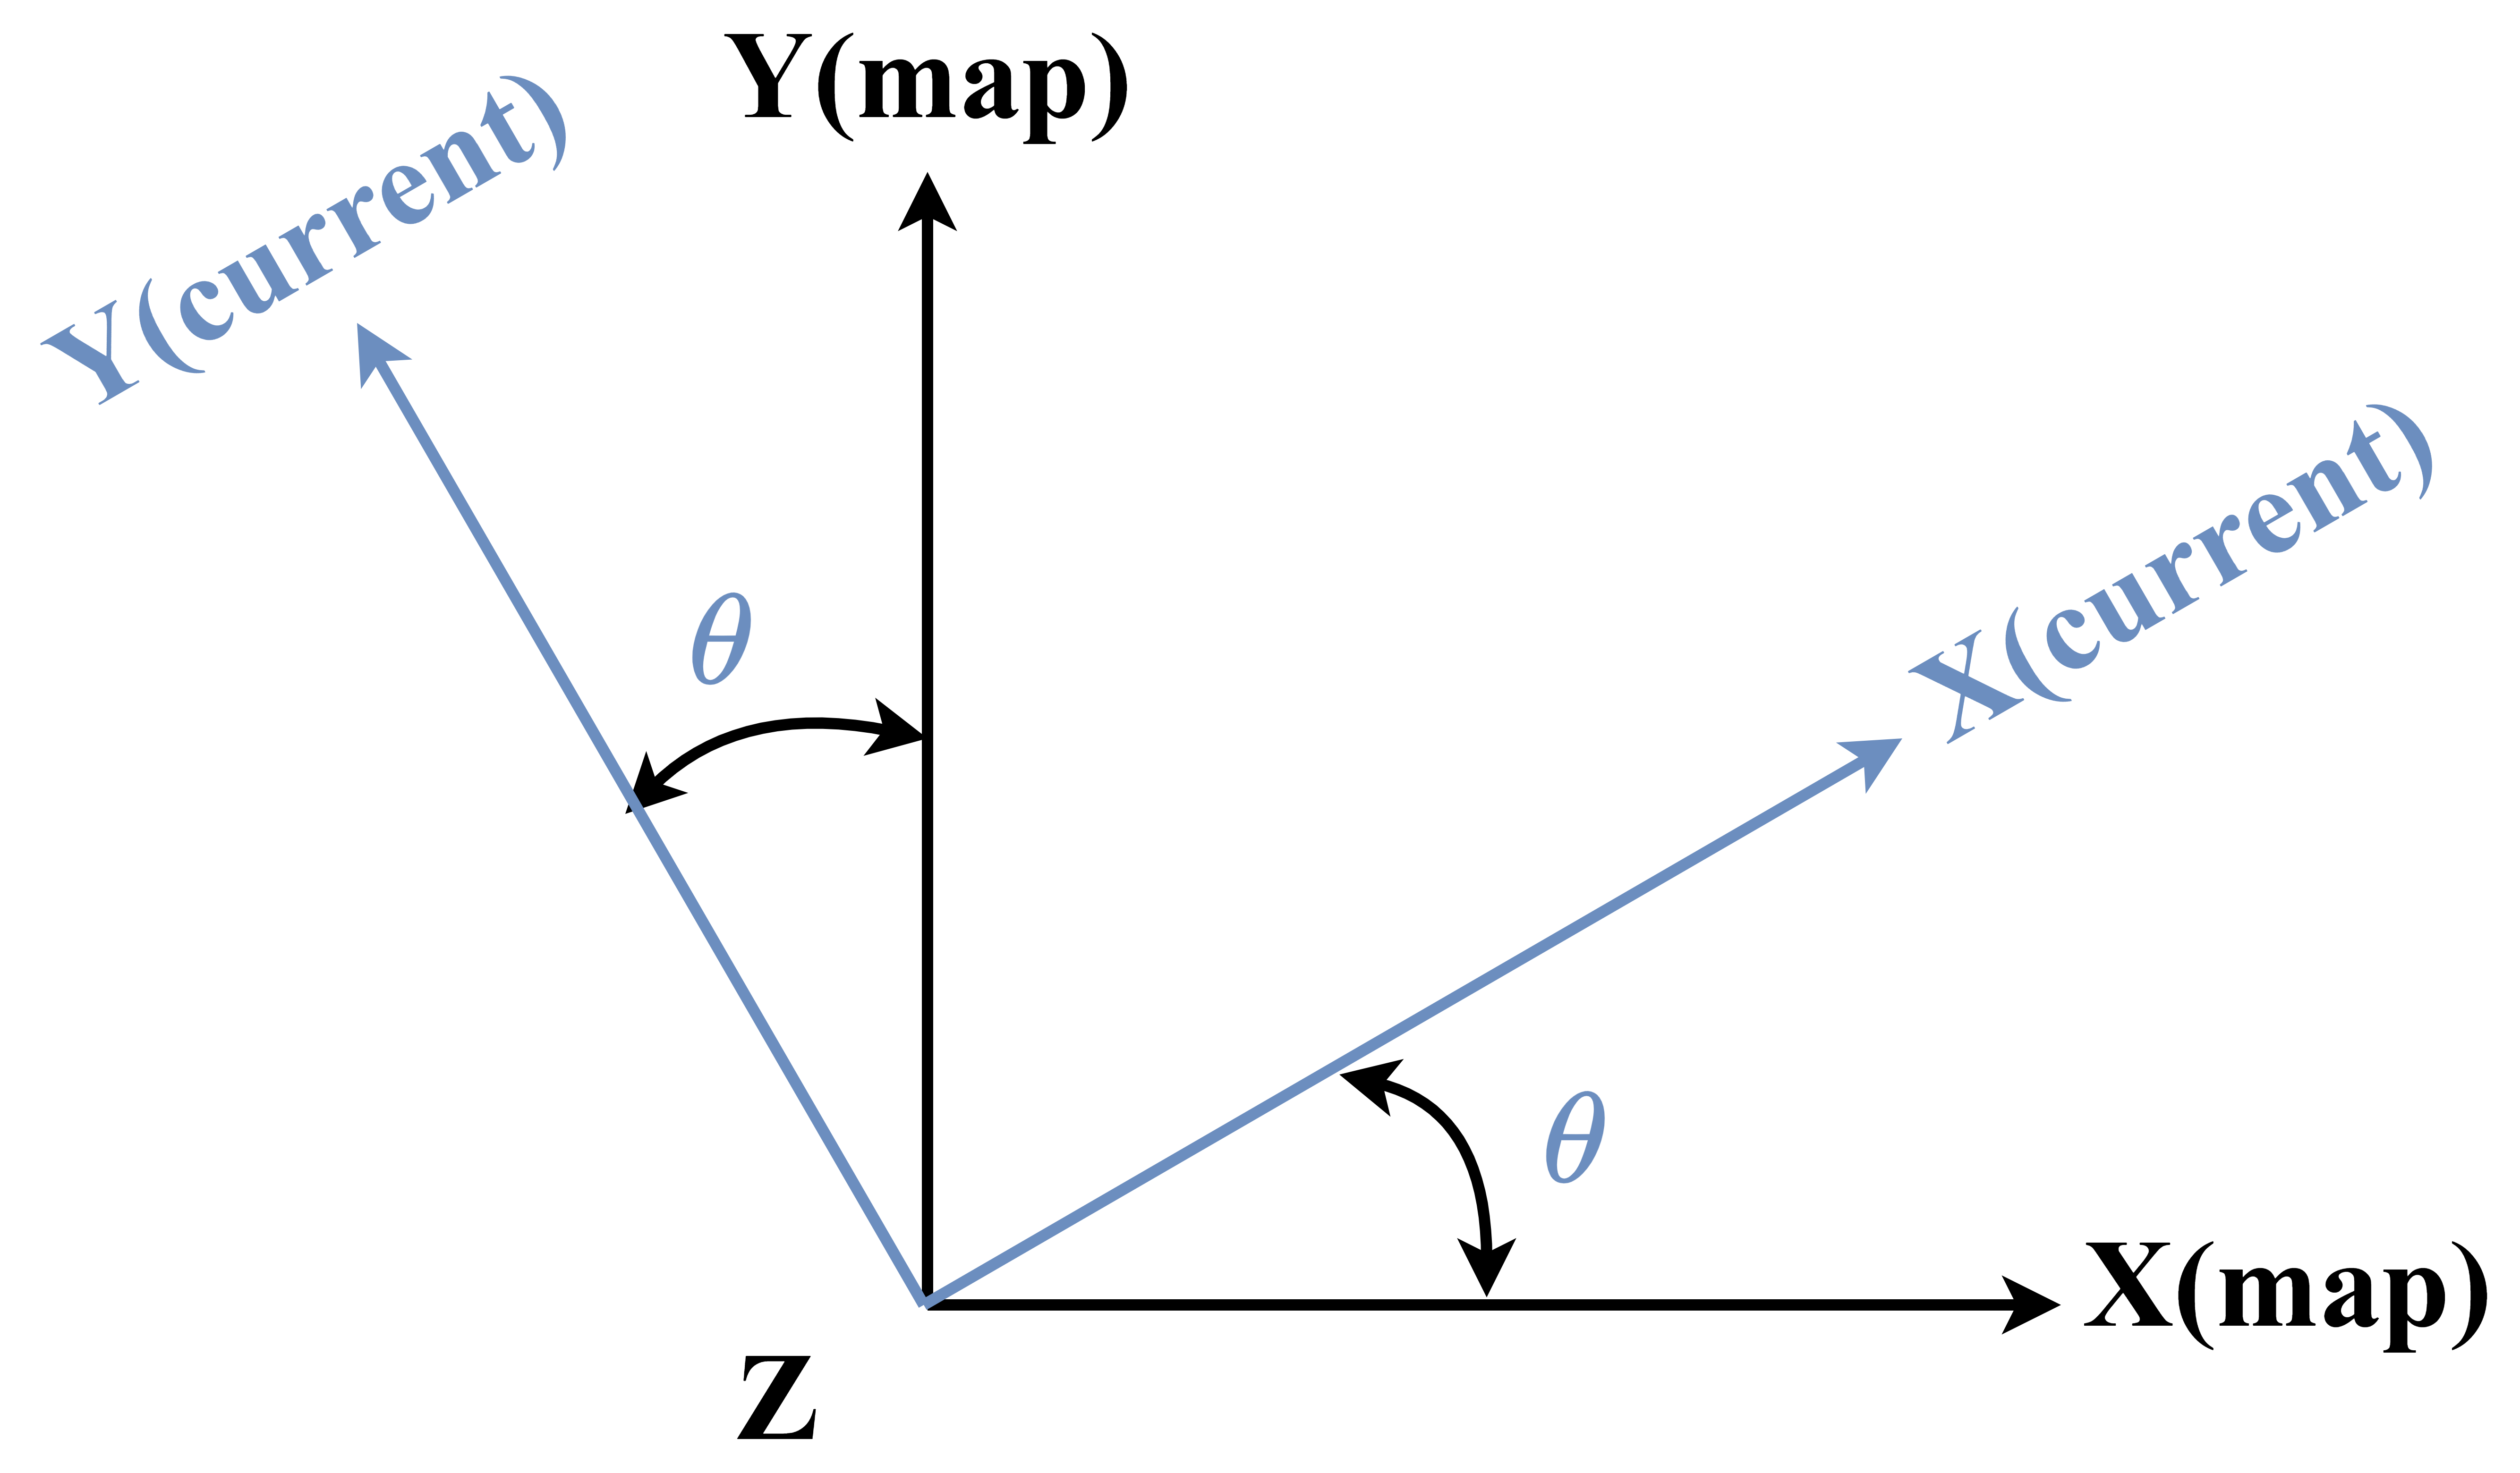
\includegraphics[scale=0.06]{Fig/axis_transform.png}
    \caption{\label{axis_transform}地图与实时位姿坐标变换}
\end{figure}
\begin{equation}
{P_B}^\prime  = \left( {\begin{array}{*{20}{c}}
{\cos \theta }&{\sin \theta }\\
{ - \sin \theta }&{\cos \theta }
\end{array}} \right)\left( {{P_B} - {P_A}} \right)
\label{myeq9}
\end{equation}
其中${{P_A}}$表示机器人在地图坐标系中的位置,${{P_B}}$表示某个导航点在地图坐标系中的位置,${P_B}^\prime$表示导航点在机器人坐标系下的相对位置,而$\theta$则表示机器人在地图坐标系中的偏航角,它代表了机器人当前位置相对于地图坐标系的旋转角度。通过计算这一角度,可以将环境中的所有导航点坐标转换为机器人坐标系中的坐标,从而确保全局路径规划中的导航点坐标是准确的。

然而,偏航角$\theta$本身无法直接测量或获得,它必须通过旋转矩阵进行求取。在ROS的Navigation框架中,可以使用tf库中的TransformListener来监听机器人在地图坐标系下的位姿信息。位姿信息是通过四元数$q = (x, y, z, w)$来表示的,其中$(x, y, z)$表示机器人的位置,而$w$则表示旋转参数。通过监听对应话题获取这一四元组后,便可以将四元组转换成式\ref{myeq10}表示的旋转矩阵$R$
\begin{equation}
	R = \left[ {\begin{array}{*{20}{c}}
		{1 - 2{y^2} - 2{z^2}}&{2\left( {xy - zw} \right)}&{2\left( {xz + yw} \right)}\\
		{2\left( {xy + zw} \right)}&{1 - 2{x^2} - 2{z^2}}&{2\left( {yz - xw} \right)}\\
		{2\left( {xz - yw} \right)}&{2\left( {yz + xw} \right)}&{1 - 2{x^2} - 2{y^2}}
		\end{array}} \right]
	\label{myeq10}
\end{equation}

除此之外,机器人当前的位姿的欧拉角是在地图坐标系下,分别通过绕X轴旋转$\gamma$角、绕Y轴旋转$\beta$角以及绕Z轴旋转$\alpha$角获得的。这些角度的组合构成了机器人在地图坐标系下的完整姿态。式\ref{myeq11}给出了旋转矩阵的计算方式,通过这个旋转矩阵可以有效地表示机器人在地图坐标系中的朝向。
\begin{equation}
	{R_{XYZ}}\left( {\gamma ,\beta ,\alpha } \right) = \left[ {\begin{array}{*{20}{c}}
		{c\alpha  \cdot c\beta }&{c\alpha  \cdot s\beta  \cdot s\gamma  - s\alpha  \cdot c\gamma }&{c\alpha  \cdot s\beta  \cdot c\gamma  + s\alpha  \cdot s\gamma }\\
		{s\alpha  \cdot c\beta }&{s\alpha  \cdot s\beta  \cdot s\gamma  + c\alpha  \cdot c\gamma }&{s\alpha  \cdot s\beta  \cdot c\gamma  - c\alpha  \cdot s\gamma }\\
		{ - s\beta }&{c\beta  \cdot s\gamma }&{c\beta  \cdot c\gamma }
		\end{array}} \right]
	\label{myeq11}
\end{equation}
式中:${c\alpha }$表示$\cos \alpha $,${s\alpha }$表示$\sin \alpha $

通过联立式\ref{myeq10}和\ref{myeq10}可以通过四元组来表示出欧拉角$\alpha $、$\beta $和$\gamma $如式\ref{myeq12}
\begin{equation}
	\begin{array}{c}
\beta  = {\rm{Atan2}}\left( { - {r_{31}},\sqrt {r_{11}^2 + r_{21}^2} } \right)\\
\alpha  = {\rm{Atan2}}\left( {\frac{{{r_{21}}}}{{c\beta }},\frac{{{r_{11}}}}{{c\beta }}} \right)\\
\gamma  = {\rm{Atan2}}\left( {\frac{{{r_{32}}}}{{c\beta }},\frac{{{r_{33}}}}{{c\beta }}} \right)
\end{array}
\label{myeq12}
\end{equation}
其中${{r_{ij}}}$表示旋转矩阵中第i行第j列元素,${\rm{Atan2}}\left( {x,y} \right)$表示$x/y$的反正切值。

式\ref{myeq12}计算得到的角度$\alpha$,即为机器人当前位姿在地图坐标系中的偏航角$\theta$,将其代回式\ref{myeq9}进行坐标转换,可以计算出各个地图坐标系线下的导航点在机器人坐标系下的精确坐标。通过与语言模型解析的方位指令进行对比,系统能够筛选出哪些导航点位于指令所指定的方位范围内,从而剔除那些不符合指令要求的冗余导航点,为机器人提供精确的路径点序列。这一优化过程显著提升了机器人在执行视觉语言导航任务时的准确性和效率。



\section{导航点规划算法}
在拥有环境拓扑图的导航点选择任务中通常会使用Dijkstra算法进行决策,根据最短距离的贪心思路帮助移动机器人进行导航点的选择,以期更快地找到目标。然而这种方法无法将导航目标与环境物体和物体之间的位置关系结合起来,且这种导航方法大多使用于静态的导航环境之中,对于可能会因为物体的摆放而改变可导航路径的复杂环境会使得原本的拓扑图失效,降低代理导航正确率和导航效率。基于这一思路,我们给全局路径规划任务进行建模,设计了一种全新的导航点规划算法。

全局路径规划可以描述为在遵循自然语言指令中给出的目标的情况下最大化导航成功的概率。具体来说,室内导航环境可以由一系列的房间$E = {e_1},{e_2}, \ldots ,{e_k}$共同组成,环境中存在由一系列导航点$V = {v_1},{v_2}, \ldots ,{v_n}$组成的拓扑图$G$,图中的节点代表了环境中的枢纽,边的权值则代表一个节点导航到另一个的路径代价。一次导航任务$\tau  \in D$由导航环境、拓扑图、初始位姿$S$和导航指令$I$确定,因此我们将每次导航任务表示成$\tau  = \left( {E,G,S,I} \right)$。在先前的小节中我们通过指令语义提取模块对导航指令$I$进行解析,提取出导航指令中的目标序列$\bar l = {l_1},{l_2}, \ldots ,{l_n}$,导航点规划算法就是要找到一个导航点序列$\bar v = {v_1},{v_2}, \ldots ,{v_n}$,使得该序列能够最大化目标与导航点之间的匹配程度,并尽可能提高导航成功率,如式\ref{myeq13}。
\begin{equation}
	P\left( {{v_i}|{l_i}} \right)P\left( {{c_{\bar v}} = 1|\bar v} \right) = \mathop {\max }\limits_{1 \le {t_i} \le  \cdots  \le {t_n} \le n} \prod\limits_{1 \le i \le n} {p\left( {{v_{{t_i}}}|{l_i}} \right) \cdot \prod\limits_{1 \le j \le n} {{\mu ^{Dis\left( {{v_j},{v_{j + 1}}} \right)}}} } 
	\label{myeq13}
\end{equation}
其中$P\left( {{c_{\bar v}} = 1|\bar v} \right)$表示根据导航点序列$\bar v$能够完成导航的概率,$P\left( {{v_i}|{l_i}} \right)$表示导航节点${v_i}$与给定的一个目标${l_i}$相匹配的概率,该概率通过多模态融合网络进行预测输出,$\mu  \in \left( {0,1} \right)$,${{\mu ^{Dis\left( {{v_j},{v_{j + 1}}} \right)}}}$代表从导航节点${{v_{j}}}$导航到${{v_{j + 1}}}$的距离代价,即随着拓扑图中所存在的任意两个导航点${v_j}$与${v_{j + 1}}$距离的增大,他们成为自然语言指令所指示的导航任务中相邻导航点的概率越小。

为了求得式\ref{myeq13}一个最优的解${\bar v}$,我们对其进行求导,得到一个对于序列$\bar t = {t_1},{t_2}, \ldots ,{t_n}$单调递增的函数:
\begin{equation}
	R\left( {\bar v,\bar t} \right) = \sum\limits_{i = 1}^n {{\rm{CLIDP}}\left( {{v_{{t_i}}},{l_i}} \right) + \log \left( \mu  \right) \cdot \sum\limits_{j =  = 1}^{T - 1} {{\rm{Dis}}\left( {{v_j},{v_{j + 1}}} \right)} } 
	\label{myeq14}
\end{equation}
当且仅当$\left( {\bar v,\bar t} \right)$最大化式\ref{myeq14}时,可以同时使得序列${\bar v}$最大化式\ref{myeq13}

为了求得最大化式\ref{myeq13}的解$\left( {\bar v,\bar t} \right)$,可以通过构造一个辅助函数,再利用动态规划的方法得到$R$的全局最优解。综上所述,对于$\forall i \in \left\{ {0,1, \ldots ,n} \right\}$和$\forall v \in V$,定义一个辅助函数$Q\left( {i,v} \right)$,表示以$v$结尾的所有导航点序列与目标点序列$\left( {{l_1},{l_2}, \ldots ,{l_n}} \right)$匹配的的最大值:
\begin{equation}
	Q\left( {i,v} \right) = \mathop {\max }\limits_{\scriptstyle\bar v = \left( {{v_1},{v_2}, \ldots ,{v_j}} \right),{v_j} = v\atop
\scriptstyle\bar t = \left( {{t_1},{t_2}, \ldots ,{t_i}} \right)} R\left( {\bar v,\bar t} \right)
	\label{myeq15}
\end{equation}

我们通过算法\ref{algorithm2}描述了结合环境拓扑图、多模态融合网络的导航点规划算法的具体过程。从起始位姿开始,通过动态规划的方式,最大化目标匹配度和最小化路径代价,以获得全局路径规划输出的导航点序列。
\begin{algorithm}[!h]
    \caption{导航点规划算法}
    \label{algorithm2}
    \renewcommand{\algorithmicrequire}{\textbf{Input:}}
    \renewcommand{\algorithmicensure}{\textbf{Output:}}
    \renewcommand{\algorithmiccomment}[1]{\hfill $\triangleright$ #1}
    \begin{algorithmic}[1]
        \REQUIRE 目标序列$\bar l = {l_1},{l_2}, \ldots ,{l_n}$,拓扑图$G$,起始位姿$S$和指令$I$  %%input
        \ENSURE 导航点序列${\rm{Path}} = \left[ {\bar v = {v_1},{v_2}, \ldots ,{v_n}} \right]$   %%output
        \STATE  对$\forall i \in 1,2, \ldots ,n$和$\forall v \in V$初始化$Q\left( {i,v} \right) =  - \infty $
        \STATE  初始化$Q\left( {0,v} \right)$
        \FOR{$i \in 1,2, \ldots ,n$}
            \STATE  对$\forall v \in V$,通过递推公式求解$Q\left( {i,v} \right)$
            \STATE  Path中添加导航点$\left( {{\rm{argmax}}\left( {Q\left( {i, * } \right)} \right)} \right)$
			\STATE  $S = {\rm{argmax}}\left( {Q\left( {i, * } \right)} \right)$
        \ENDFOR
    \end{algorithmic}
\end{algorithm}

在上述的导航点规划算法中,首先输入通过语言模型提取的目标序列和环境拓扑图,设置导航起始点$S$,初始化$Q\left( {0,v} \right)$为导航起始点$S$到各个导航点$v$的最短路径长度,当$i \ge 1$时,我们通过动态规划递推公式计算每一时刻的$Q(i, v)$值:
\begin{equation}
Q\left( {i,v} \right) = \max \left( {Q\left( {i - 1,v} \right) + {\rm{CLIDP}}\left( {v,{l_i}} \right),\mathop {\max }\limits_{\omega  \in {\rm{neighbors}}\left( v \right)} \lambda  \cdot Q\left( {i,\omega } \right) + \mu  \cdot Dis\left( {v,\omega } \right)} \right)
	\label{myeq16}
\end{equation}
其中,${{\rm{neighbors}}\left( v \right)}$表示拓扑图中节点$v$的邻接点,$\lambda  \in \left( {0,1} \right)$表示缩放参数,目的是减少先前的导航点选择对后续决策的影响。在每一次的递推过程中,我们采用贪心策略选取能够使得$Q\left( {i,v} \right)$取得最大值、且经过方位优化筛选后的节点作为当前目标所对应的导航点,并将其设为下一递推过程的起点,直到遍历完目标序列,得到全局路径规划的导航点序列$\bar v = {v_1},{v_2}, \ldots ,{v_n}$。




\section{本章小结}
本章主要内容是目标物体导航过程中涉及到的一些常用的网络在导航过程中的作用以及这些网络的算法原理和操作流程,主要介绍了指令语义提取模块、多模态融合网络模块、方位优化算法和导航点规划算法。




%第三章
	\chapter{局部路径规划导航方法}
本章将详细介绍LVL-Nav方法中的局部路径规划导航方法,包含描述全局路径规划方法不足之处的引言,针对该不足所提出的局部路径规划方法的导航框架设计,最后分别描述了框架中的特征提取模块、特征融合模块、运动模块和图像点云融合模块四个主体部分。


\section{引言}

目标物体导航方法旨在使移动机器人能根据自然语言指令中的多种目标进行导航,并要求机器人能够导航至目标位置的半米范围内。使机器人能够理解和执行指令是完成这一任务的关键之一,但基于导航点的全局路径规划导航方法侧重于将移动机器人引导到环境中预设的导航点,在许多应用场景中实际选取的导航点可能只是路径上的中转位置,仅仅代表该点距离目标较近而不代表机器人已经到达最终的实际目标旁。出于这类方法的限制,我们所提出的全局路径规划方法在目标没有明确的预设导航点的情况下无法十分有效地应对需要精确导航到目标物体的任务。
除此之外,在未知或动态变化的环境中机器人需要能够根据感知信息实时地调整自己的路径并同时发现和定位到目标物体。传统的导航方法并不具备让机器人在局部环境中进行自主探索的能力,无法完成机器人在未知环境中的探索任务。
因此要在更复杂的应用场景中实现精准的导航,移动机器人不仅需要依赖于导航点的引导,还需要具备自主探索、识别目标并作出相应决策的能力。

在现有的视觉语言导肮方法中,
2020年,Krantz\cite{krantz2020beyond}等人开发了序列到序列的基准模型和能够融合多种特征的多模态注意模型,用以完成连续环境中的视觉语言导航。
Du\cite{du2020learning, du2021vtnet}等人提出了基于视觉神经网络的目标物体导航方法,使用Transformer表征环境特征并输入强化学习网络学习导航策略,降低了模型训练时的试错成本。
Wang\cite{wang2021visual}等人为了解决不同机器人之间难以传递导航技能而提出了一种基于元学习的视觉感知泛化策略,在视觉感知模型中分别使用与模型无关的元学习算法和基于指标的元学习算法,以便在可见和不可见的环境中更好地泛化,使智能体能够快速适应新的相机配置。
Fang\cite{fang2022target}等人提出了一种基于强化学习的目标物体导航方法,提高了智能体的泛化能力。
Fukushima\cite{fukushima2022object}等人提出基于对象记忆Transfomer的目标物体导航方法,使用对象场景存储器存储长期场景和对象序列,实现室内环境高效导航。
朱威\cite{朱威2024结合优势结构和最小目标}等人提出了一种结合优势结构和最小化目标Q值的深度强化学习导航算法,加快多目标连续导航训练过程中的收敛速度。
这类方法基本都采用从视觉观察中提取物体语义、物体位置和相对位置等特征信息,将其通过编码的嵌入层网络以构建丰富的视觉表示,以此来告诉模型周围环境的特征。除此之外模型还会关注当前视觉观察中与目标物体相关联的区域的方向信息,这使得代理能够朝着正确的方向进行探索导航。

根据上述的问题和已有的解决思路,本章提出了一种局部路径规划方法。我们的目标是根据指令中目标物体的名称,通过特征融合、特征提取网络模型输出的离散动作在局部环境中进行自主探索,同时利用视觉图像信息识别出目标物体,在视觉观察中定位目标物体后再由图像点云融合算法计算获得目标的精确位姿,转换坐标系后发布导航任务完成局部环境目标物体导航。该方法由特征提取模块、特征融合模块、运动模块和图像点云融合模块构成。


\section{导航框架设计}
未知环境下视觉导航系统需要实现未知环境探索、动作执行和图像点云融合导航三个方面的功能,因此我们设计了由未知环境探索节点、运动节点、图像点云融合节点构成的局部路径规划导航系统,如图所示\ref{局部路径规划导航方法}。

其中,未知环境探索节点由多模态特征提取器与跨模态融合器一同组成,该节点基于Transformer的并行注意力架构对视觉观察的场景特征向量与目标对象语义描述特征进行融合,进而生成用以描述导航方向指引向量以及表征空间拓扑结构的环境特征。接着,在ROS机器人导航框架之下通过动作执行节点封装可能执行的离散环境探索动作,以期找到导航目标,当发现目标时则进入图像点云融合节点,通过点云聚类算法、目标检测算法和IoU度量算法获得精准的目标物体的位置信息,最后发布导航任务完成目标物体导航。
\begin{figure}[htbp]
    \centering
    \includegraphics[scale=0.05]{Fig/未知环境导航框架.png}
    \caption{\label{局部路径规划导航方法}局部路径规划导航框架}
\end{figure}

具体来说,特征提取模块采用预训练参数初始化的残差卷积网络来解析场景的宏观语义表征,同时通过基于注意力机制的检测模型捕获包含局部对象的语义分布及其几何编码信息在内的细粒度区域感知特征,并通过参数化嵌入映射层来生成具有可解释性的目标特征向量。接着,在特征融合模块中对全局特征、局部特征和目标特征进行融合,将获得的方向特征、环境特征和上一时刻的动作特征通过LSTM网络进行编码生成导航动作和动作评分,通过运动模块中封装好的离散动作函数进行执行,以此来指导代理在局部未知环境中进行探索。
接着,在视觉和多线激光雷达进行联合标定并确定发现目标后,通过YOLOV10目标检测算法认知环境中存在的目标的同时,再通过点云聚类感知获得目标与移动机器人之间的相对位置信息,通过图像点云融合模块获得目标位姿,再经过坐标变换得到目标在map坐标系下的坐标。最后再运动模块中利用Navigation导航框架发布导航任务完成导航到目标旁以完成局部导航,进一步完成移动机器人执行导航的闭环任务。

未知环境下的导航探索主要由特征提取模块和特征融合模块构成,如图\ref{提取-融合框架},其中特征提取模块从移动机器人上的单目相机获取第一人称环境视觉图像,并将其送入不同的特征提取网络中,分别提取表征各个区域物体语义、位置信息的$100 \times 256$局部特征、表征导航环境中机器人所处位置的位姿信息的$49 \times 256$全局特征和表征探索导航目标的$1 \times 256$目标特征。接着再通过主要由encoder特征强化、decoder特征融合和LSTM这三个结构组成的特征融合模块生成表征离散动作空间的动作概率分布函数。具体来说特征融合模块将特征提取获得的三个不同特征进行强化融合,并通过LSTM网络进行导航序列建模以生成$1 \times 4$的动作特征,最后由运动模块进行探索任务。
\begin{figure}[htbp]
    \centering
    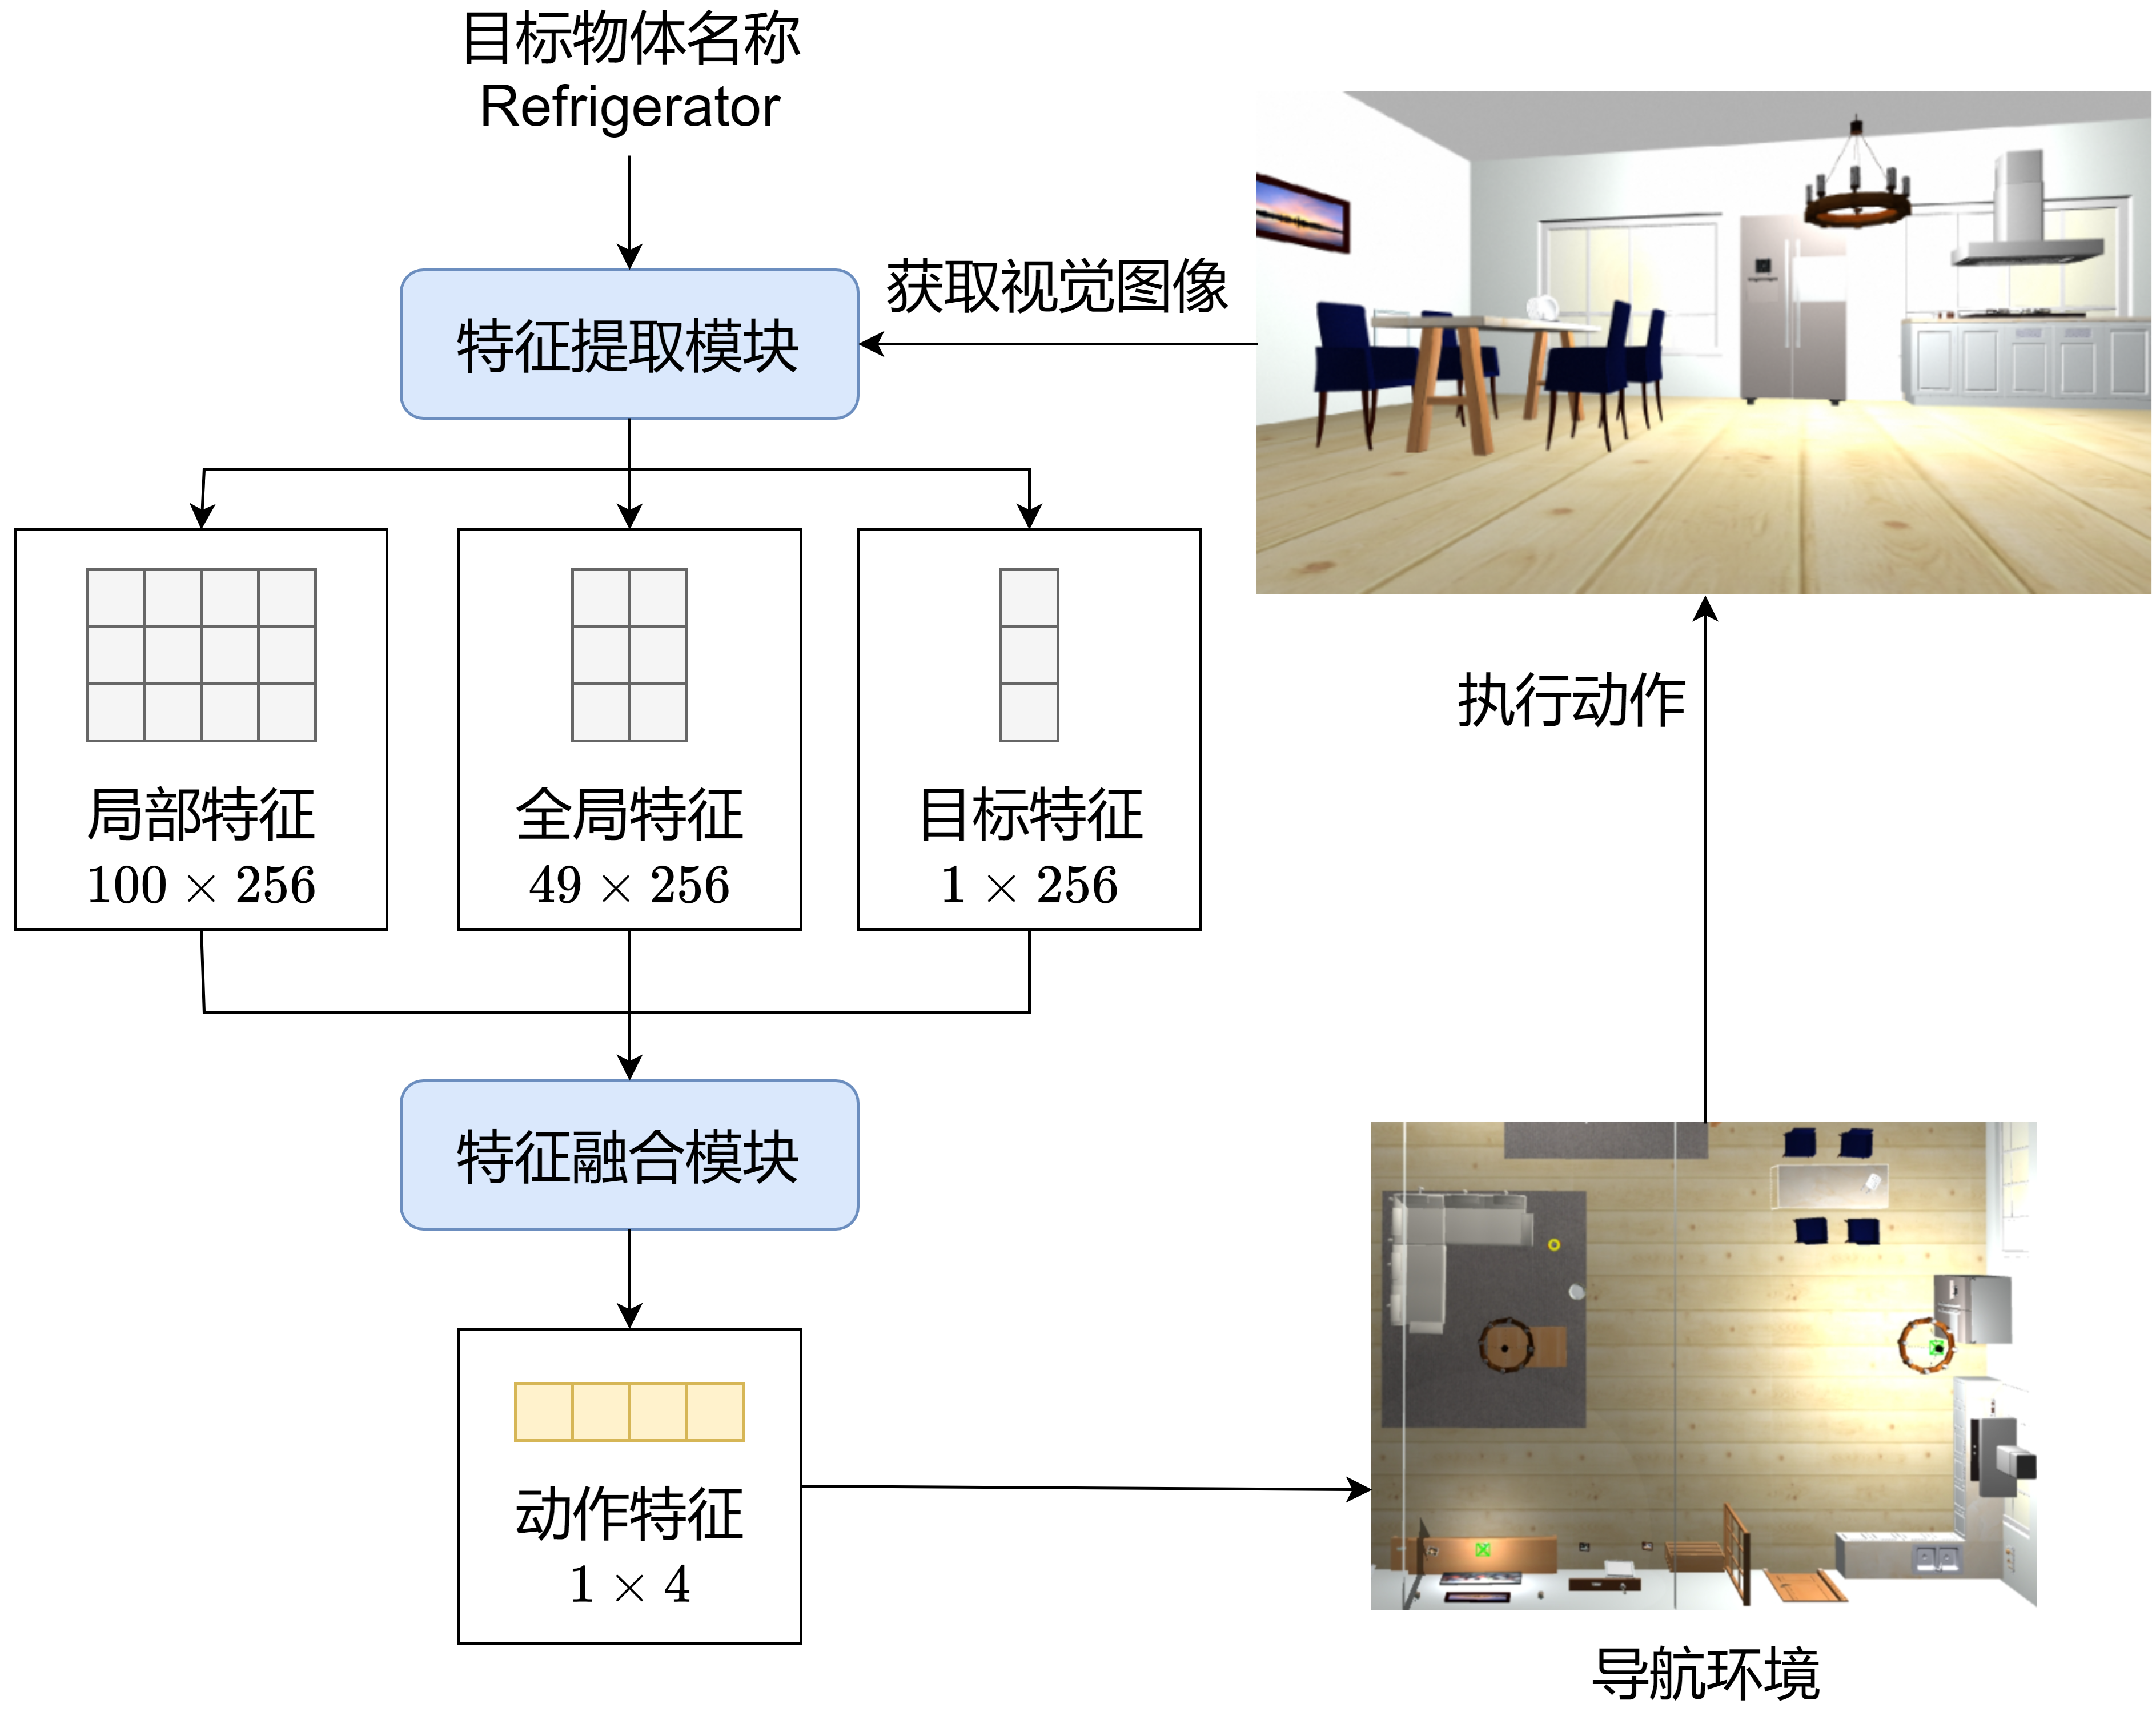
\includegraphics[scale=0.07]{Fig/提取-融合框架.png}
    \caption{\label{提取-融合框架}未知环境下的导航探索框架}
\end{figure}

上述操作过程可以用公式表示为
\begin{equation}
    {X_{{\rm{local}}}},{X_{{\rm{global}}}},{X_{{\rm{target}}}} = Extract\left( {{X_{{\rm{image}}}},{X_{{\rm{text}}}}} \right)
    \label{myeq30}
\end{equation}
\begin{equation}
    {X_{{\rm{action}}}} = Fusion\left( {{X_{{\rm{local}}}},{X_{{\rm{global}}}},{X_{{\rm{target}}}}} \right)
    \label{myeq31}
\end{equation}
其中$Extract\left( {} \right),Fusion\left( {} \right)$分别表示特征提取模块、特征融合模块,${X_{{\rm{local}}}},{X_{{\rm{global}}}},{X_{{\rm{target}}}},{X_{{\rm{image}}}},{X_{{\rm{text}}}},{X_{{\rm{action}}}}$分别表示特征提取模块中的局部特征、全局特征、目标特征、第一人称视觉图像、输入目标和特征融合模块的动作特征。



\section{特征提取模块}
在未知环境的探索导航过程中使用多层次的特征提取策略能够充分利用环境信息,使机器人在无先验知识的情况下更高效、可靠地探索并接近目标。
在未知环境下的探索导航过程中,特征提取模块主要由三个分别提取局部特征、全局特征和目标特征的不同网络组成,可以用公式表示为
\begin{equation}
{X_{{\rm{local}}}} = Concat\left( {ReLU\left( {Linear\left( {DETR\left( {{X_{{\rm{image}}}}} \right)} \right)} \right),{X_{{\rm{corelation}}}}} \right)
    \label{myeq32}
\end{equation}
\begin{equation}
{X_{{\rm{global}}}} = Flatten\left( {Conv\left( {ResNet\left( {{X_{{\rm{image}}}}} \right)} \right) + {X_{{\rm{position}}}}} \right)
    \label{myeq33}
\end{equation}
\begin{equation}
{X_{{\rm{target}}}} = Embedding\left( {{X_{{\rm{text}}}}} \right)
    \label{myeq34}
\end{equation}

经过特征提取模块处理后,提取出的的用于描述局部场景内物体语义属性及方位信息的区域特征、描述整体环境状态的全局特征以及反映待识别目标语义特性的对象特征均被标准化为256维向量并集成于同一嵌入空间之中。这一对齐操作有效促进了多模态特征的协同交互,为后续特征融合环节构建视觉观测数据与目标实体间的深度语义关联奠定了结构基础,能够实现异构特征的高效融合。

\subsection{提取局部特征}
局部特征的提取流程如图\ref{局部特征提取}所示。在一开始我们使用预训练的DETR网络来提取第一人称视觉图像,用于表征当前视觉观察的局部信息、帮助代理认知视觉观察图像中物体代表的语义信息和位置信息,得到$100 \times 256$的局部特征,其中我们的DETR网络使用ResNet-50作为主干网络,采用六层编码器、六层解码器、八个独立注意力头和维度为2048的前馈神经网络搭建而成。然后将该特征经过全连接层Linear和ReLU激活函数以得到$100 \times 249$的局部特征,再将表征推理结果的$100 \times 7$关联特征与局部特征进行连接,得到包含环境所存在的物体语义信息、位姿信息、可靠性在内的$100 \times 256$的局部特征。
\begin{figure}[htbp]
    \centering
    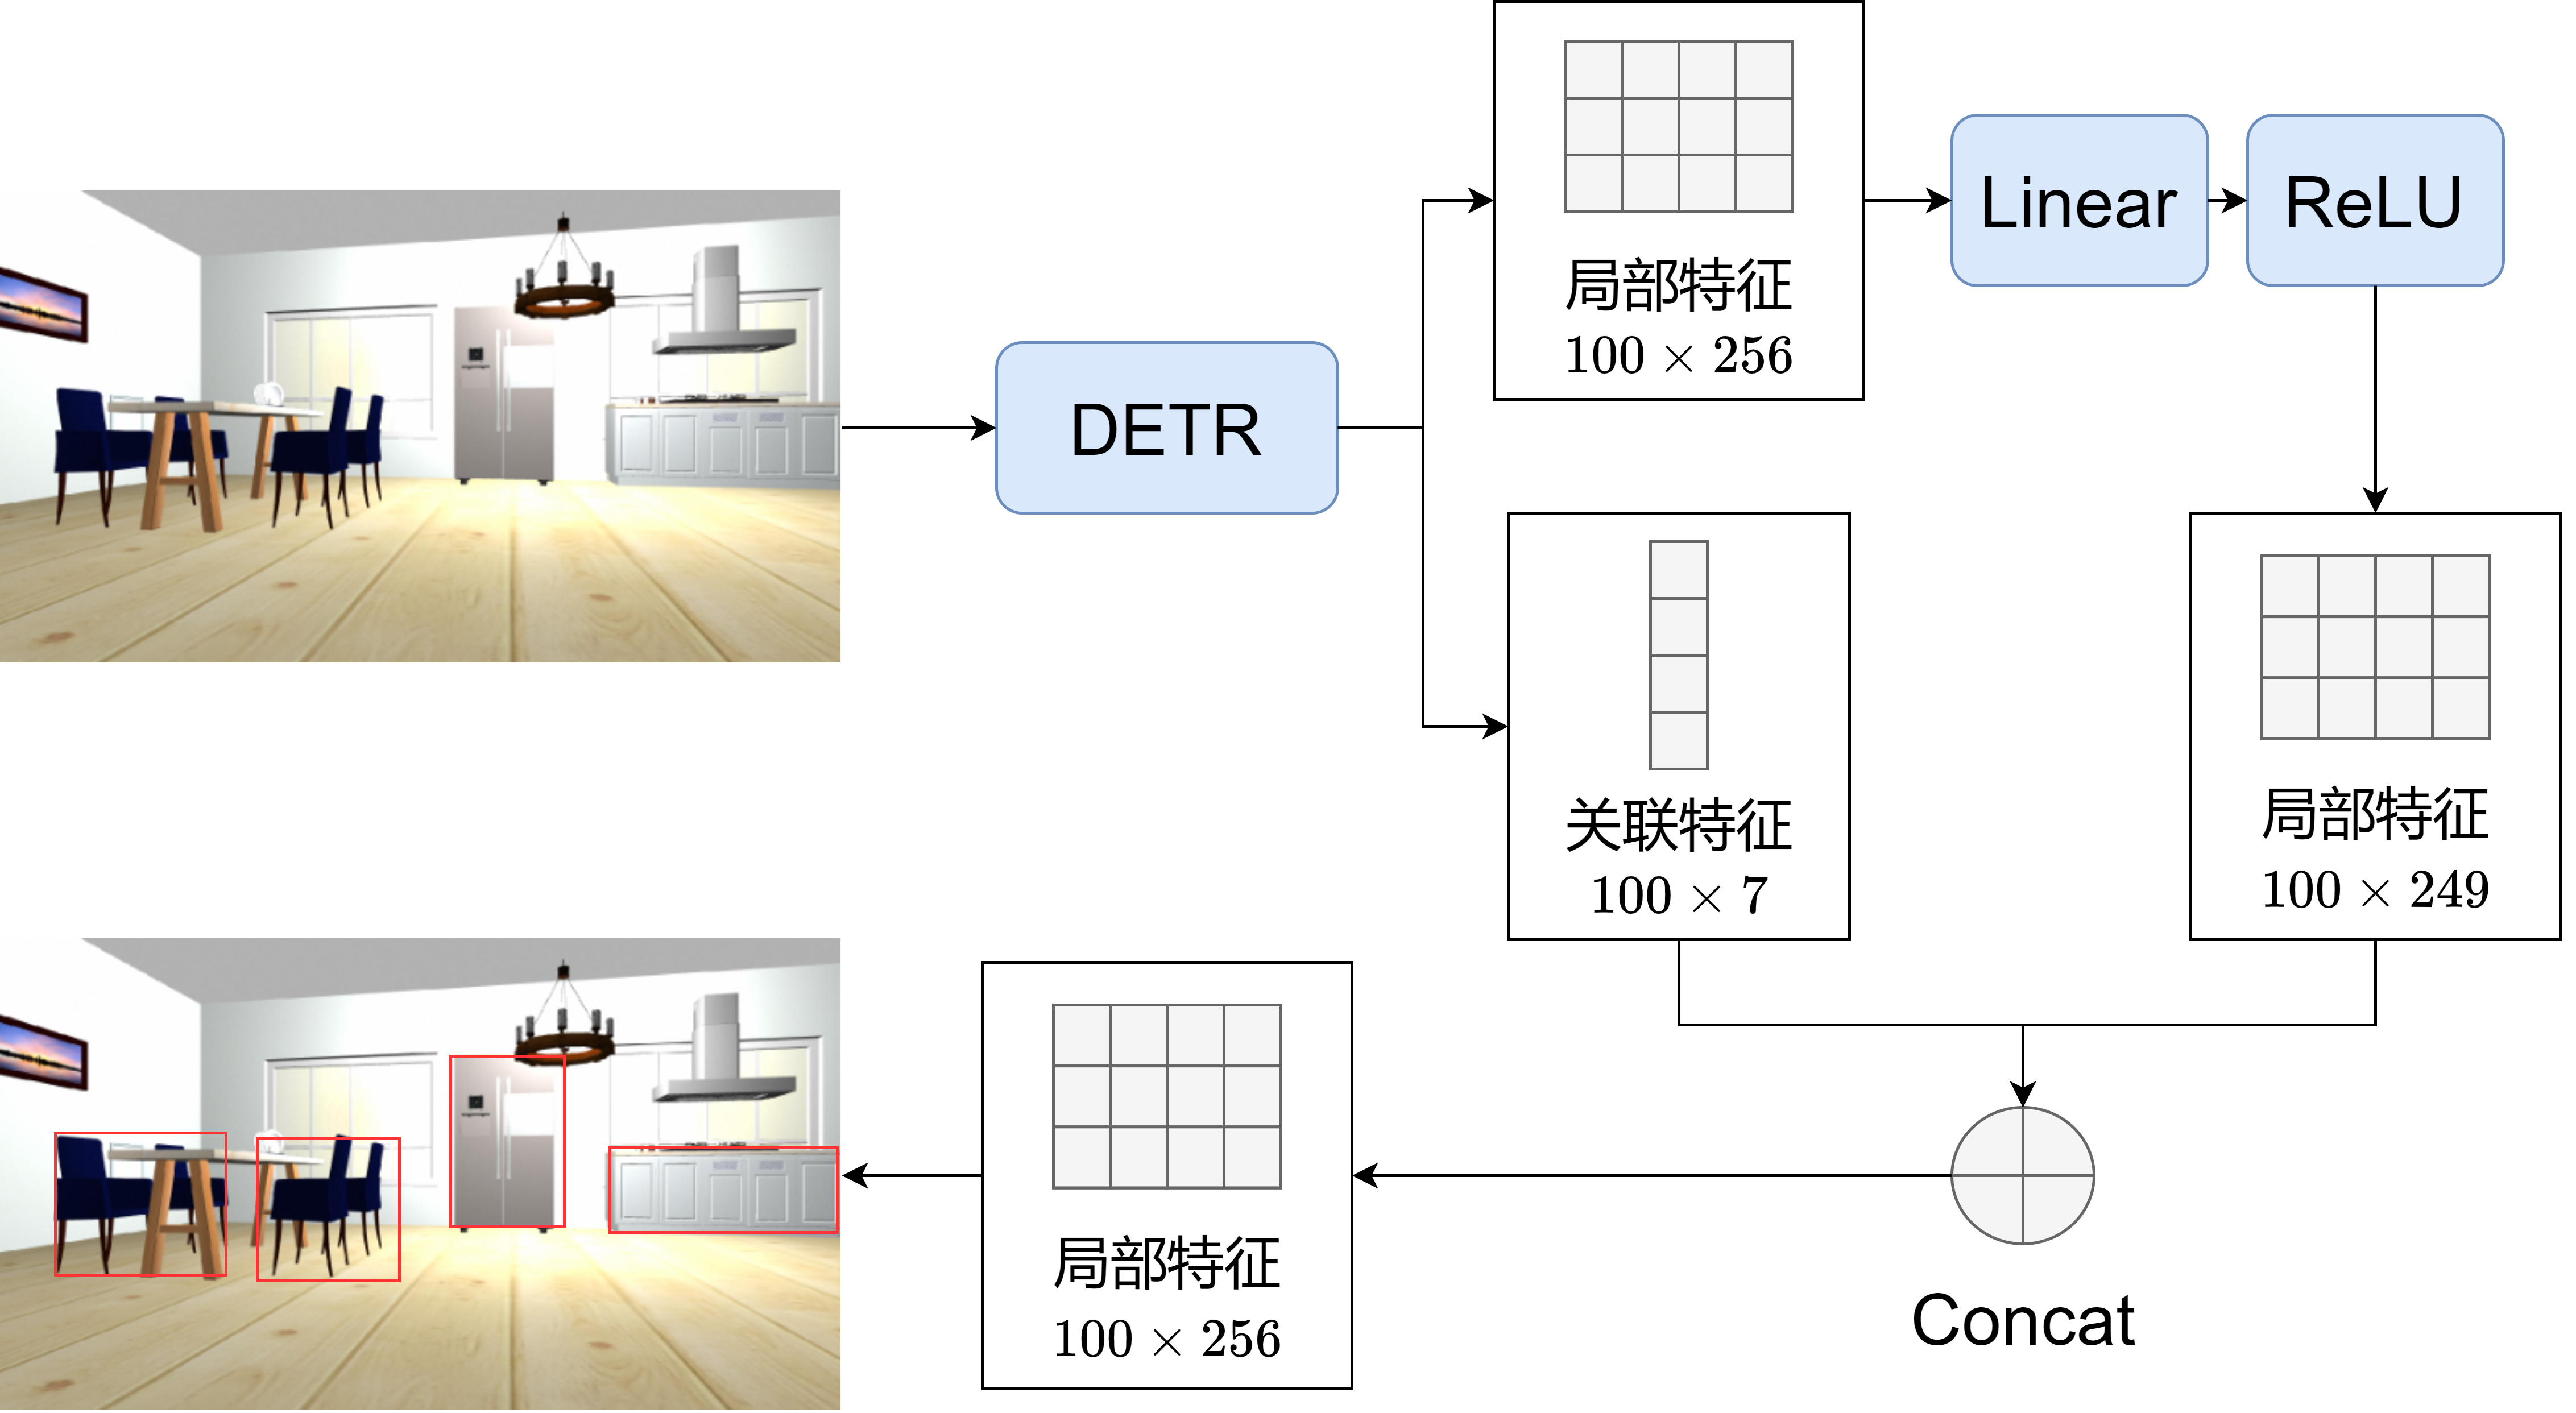
\includegraphics[scale=0.06]{Fig/局部特征提取.png}
    \caption{\label{局部特征提取}局部特征提取流程}
\end{figure}

\subsection{提取全局特征}


全局特征的提取流程如图\ref{全局特征提取}所示。我们构建了基于ResNet18架构的特征提取网络用于解析机器人本体视角采集的RGB图像数据。该编码器通过深度卷积网络提取场景的空间拓扑表征来为智能体提供空间定位的环境认知信息。首先使用斯坦福大学开源的ImageNet数据集对我们搭建的ResNet18网络进行预训练,将第一人称观察视觉图像输入到该预训练的网络中再经过Conv卷积层和ReLU激活函数得到$7 \times 7 \times 256$的全局特征,然后将输出的环境表征张量与三角函数位置嵌入生成的$7 \times 7 \times 256$维位置编码矩阵进行Add操作和Flatten操作得到维度为$49 \times 256$的融合特征向量以完成多模态感知信息的空间对齐。其中正余弦位置编码是一种固定、无训练参数的编码方法,它可以表示为式\ref{myeq35}、\ref{myeq36},其中pos表示位置索引,i表示特征维度索引,$d_{{\rm{model}}}$表示嵌入维度即模型隐藏层维度,分母${10000^{{{2i} \mathord{\left/
 {\vphantom {{2i} {{d_{{\rm{model}}}}}}} \right.
 \kern-\nulldelimiterspace} {{d_{{\rm{model}}}}}}}}$表示用于确保不同维度的编码值在不同的频率范围内变化的缩放因子。
\begin{figure}[htbp]
    \centering
    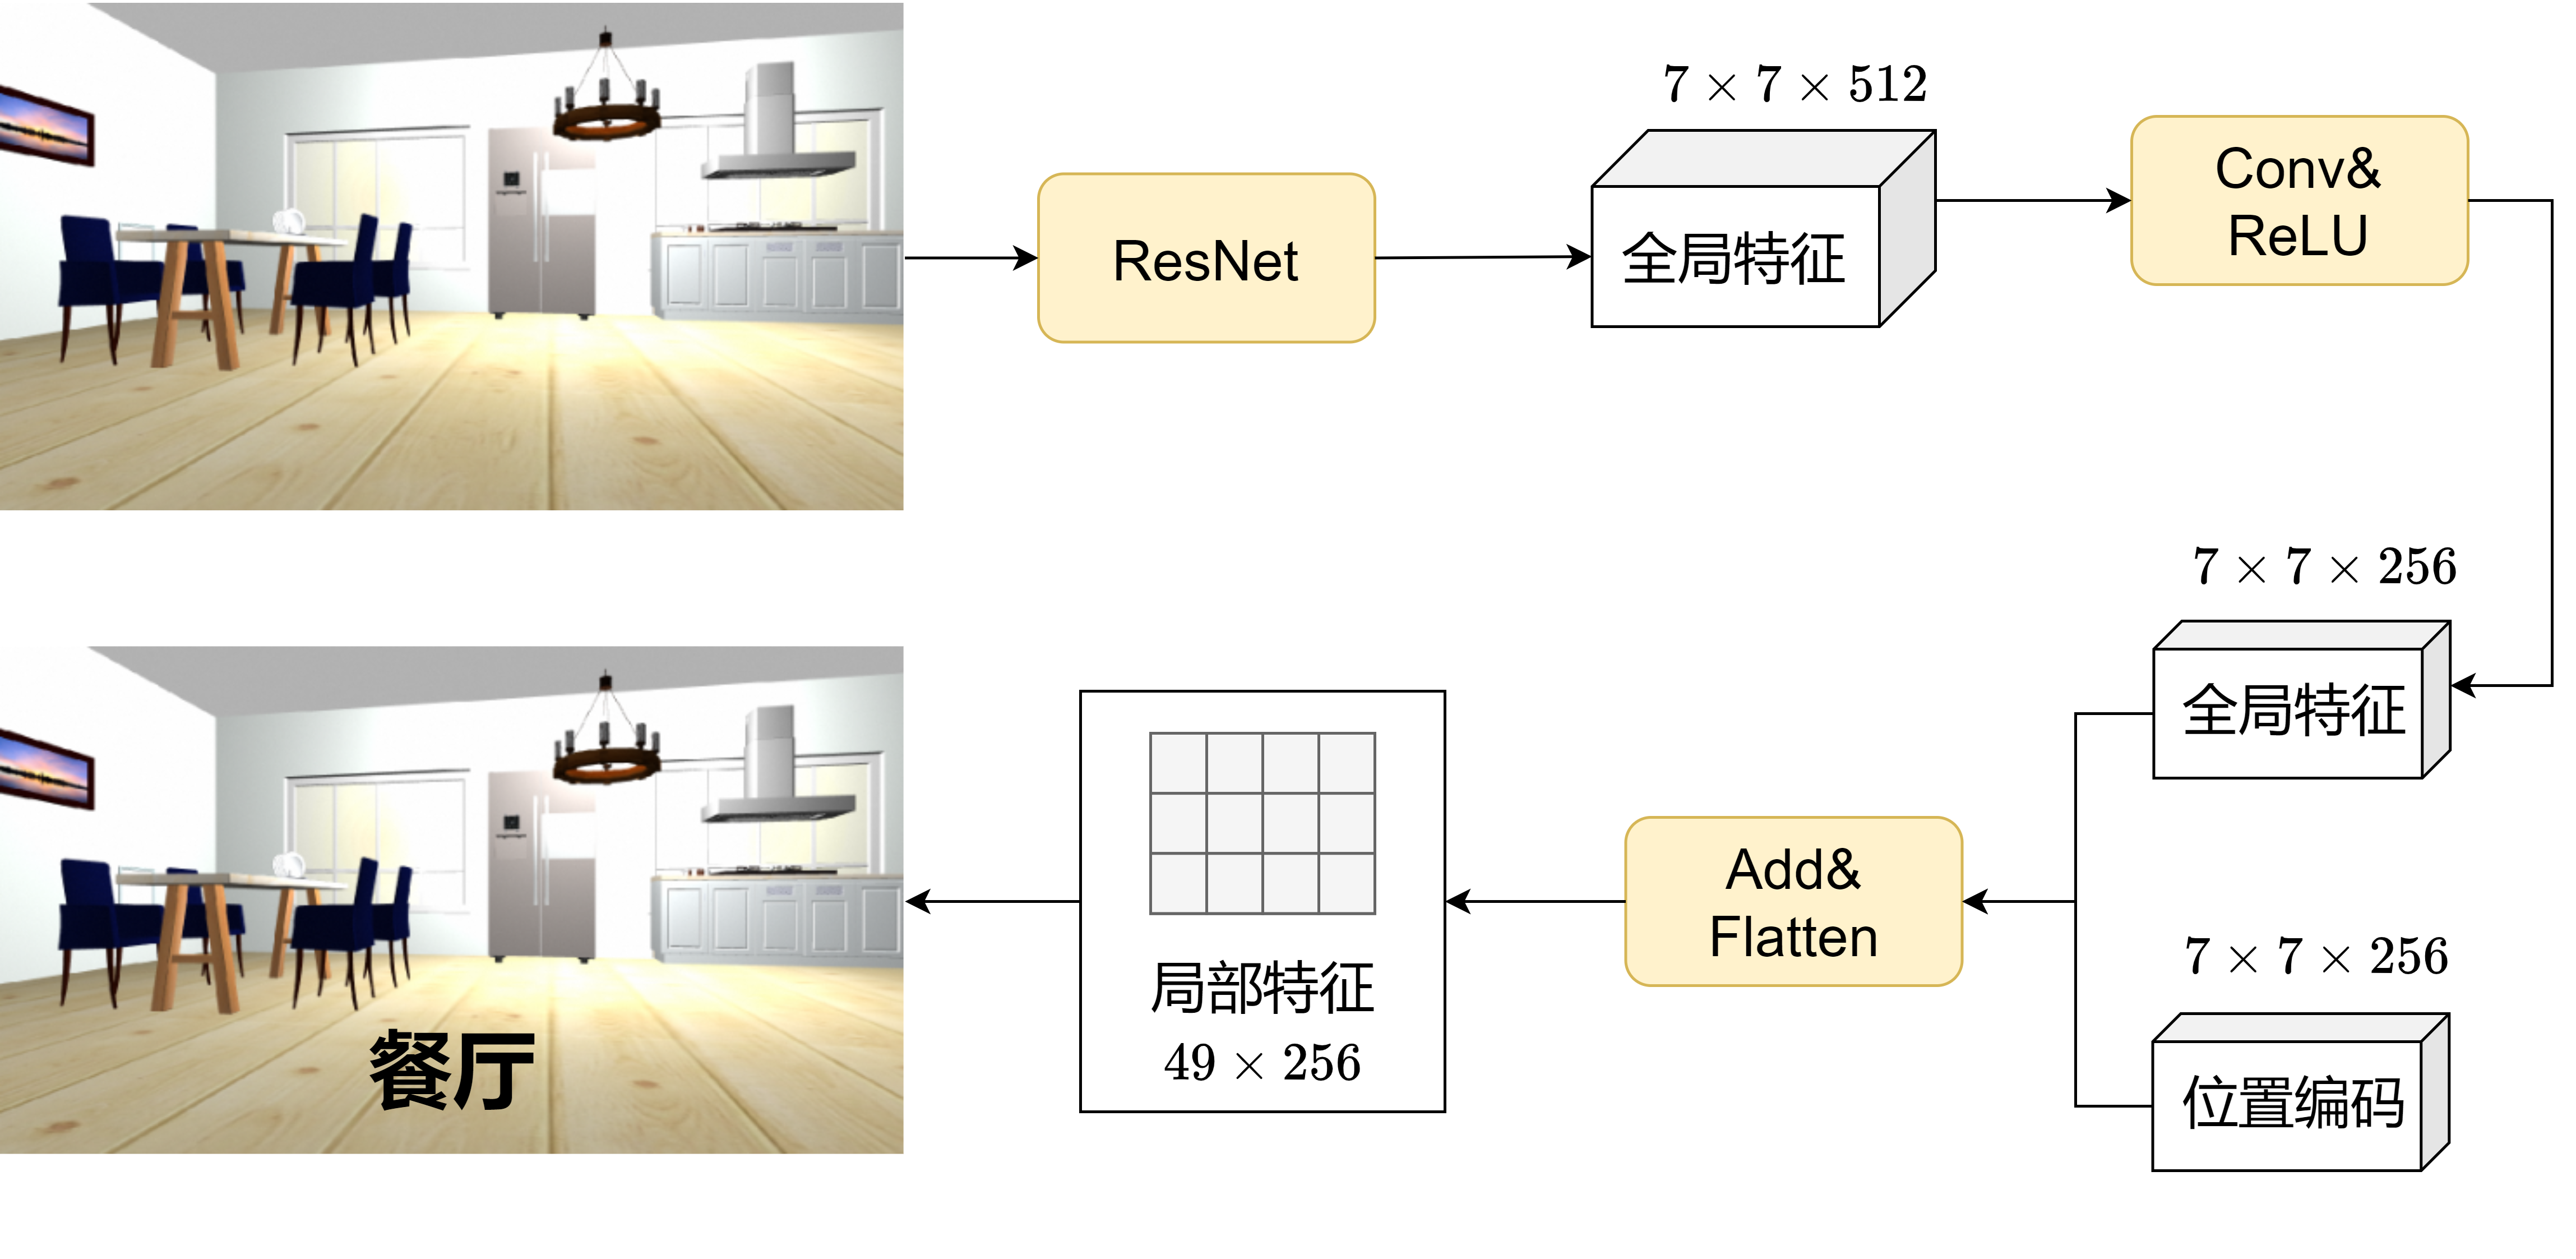
\includegraphics[scale=0.06]{Fig/全局特征提取.png}
    \caption{\label{全局特征提取}全局特征提取流程}
\end{figure}

\begin{equation}
    P{E_{\left( {pos,2i} \right)}} = \sin \left( {\frac{{pos}}{{{{10000}^{{{2i} \mathord{\left/
 {\vphantom {{2i} {{d_{{\rm{model}}}}}}} \right.
 \kern-\nulldelimiterspace} {{d_{{\rm{model}}}}}}}}}}} \right)
    \label{myeq35}
\end{equation}
\begin{equation}
    P{E_{\left( {pos,2i + 1} \right)}} = \cos \left( {\frac{{pos}}{{{{10000}^{{{2i} \mathord{\left/
 {\vphantom {{2i} {{d_{{\rm{model}}}}}}} \right.
 \kern-\nulldelimiterspace} {{d_{{\rm{model}}}}}}}}}}} \right)
    \label{myeq36}
\end{equation}

\subsection{提取目标特征}
目标特征提取流程如图\ref{目标特征提取}所示。我们在特征构建阶段定义词表容量$V = 32$与嵌入空间维度D=256作为核心超参数并以此初始化嵌入矩阵$M$,接着通过输入目标实体在词表中的离散索引$I$来执行嵌入层的索引查询操作,从映射关系矩阵$M$中抽取对应的目标语义向量进而完成符号空间到连续向量空间的转换。在训练过程中,该目标特征会不断被优化,使语义相近的信息在嵌入空间中更加接近,从而增强特征融合模块在构建文本语义与视觉语义关联方面的能力。利用嵌入层网络对目标物体的单词进行编码可以生成用于指代目标物体语义的目标特征。在后续的特征融合过程中,可以借助注意力机制筛选出视觉观察中与目标物体相关的物体特征,从而精准确定导航的方向以快速在未知环境中找到目标。
\begin{figure}[htbp]
    \centering
    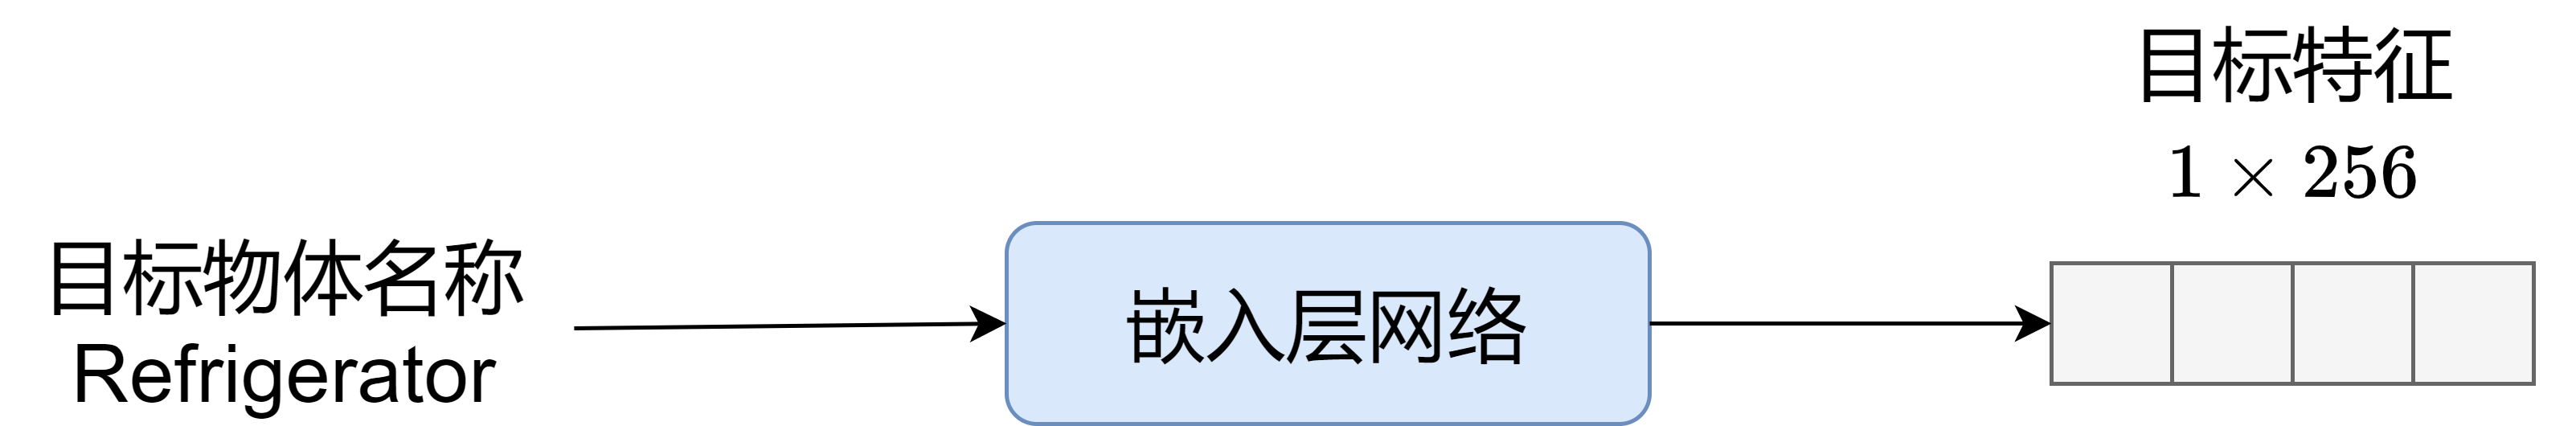
\includegraphics[scale=0.10]{Fig/目标特征提取.png}
    \caption{\label{目标特征提取}目标特征提取流程}
\end{figure}



\section{特征融合模块}
特征融合模块主要由特征融合编码器、特征融合解码器和LSTM网络构成。其中特征融合编码器主要由具有自注意力机制的Transformer encoder组成,它将特征提取模块获得的局部特征通过自注意力机制编码强化,获得能够表征表示物体与一和位置信息的强化局部特征,并将其作为键值对输入到特征融合解码器之中。特征融合解码器同样由具有多头自注意力机制的Transfomer decoder组成,它将表征目标物体语义信息和机器人所处环境位置信息的目标特征和全局特征进行强化编码,然后将作为键值对的局部特征与他们连结而成查询一同输入到网络之中,通过decoder进行融合得到环境特征和方向特征,最后,经过LSTM网络输出代理在未知环境下进行探索的离散导航动作。

我们通过观察人类在环境中寻找目标物体的过程发现,当目标物体出现在视觉观察范围内时,我们会直接按照最近的路线去靠近目标,而当目标物体未出现在观察范围内时,我们则会前往环境中存在的所有物体中与目标关联性最强的物体附近进行寻找。我们按照这样的思路去搭建特征融合网络以指导代理能够更精准的在局部未知环境中进行导航,如图\ref{未知环境导航示例图}所示,环境中存在硬纸盒、手提电脑和花盆三个物体。当需要导航到视觉观察中所发现的目标物体花盆时,代理就会根据标目标物体出现在视觉观察中的位置进行决策,执行向右前方进行移动的动作。当需要导航到视觉观察中未出现的目标物体鼠标时,代理则会先判断视觉观察中所出现的所有物体与目标物体的关联性,然后导航到手提电脑这一最可能会找到鼠标的目标旁。
\begin{figure}[htbp]
    \centering
    \includegraphics[scale=0.07]{Fig/导航示例图.png}
    \caption{\label{未知环境导航示例图}未知环境导航示例图}
\end{figure}

因此,为了使移动机器人能够正确定位其当前所在位置,需要从视觉观察中提取环境特征,同时还需要提取局部特征以感知周围环境中物体的语义信息和位置信息。此外,代理应建立目标特征与全局特征、局部特征之间的紧密关联,从而有效引导方向特征的生成。同时,还需融合当前的全局特征与局部特征以获取环境的整体表征,并构建方向特征与环境特征相对应的序列,为后续模块提供历史经验信息,帮助LSTM网络正确地输出导航动作以指导代理在局部未知环境中进行精准高效的导航。特征融合模块的操作流程可以用如下公式表示,其中$Encoder$表示特征融合编码器,$Decoder$表示特征融合解码器。
\begin{equation}
{X_{{\rm{encoder}}}} = Encoder\left( {{X_{{\rm{local}}}}} \right)
    \label{myeq37}
\end{equation}
\begin{equation}
    {X_{{\rm{direction}}}},{X_{{\rm{environment}}}} = Decoder\left( {Concat\left( {{X_{{\rm{global}}}},{X_{{\rm{target}}}},{X_{{\rm{parameter}}}}} \right),{X_{{\rm{encoder}}}}} \right)
    \label{myeq38}
\end{equation}
\begin{equation}
    X_{{\rm{action}}}^n = Linear\left( {LSTM\left( {{X_{{\rm{direction}}}},{X_{{\rm{environment}}}},X_{{\rm{action}}}^{n - 1}} \right)} \right)
    \label{myeq39}
\end{equation}

\subsection{特征融合编码器}
特征融合模块中的编码、解码器基于Transfomer进行搭建,它的参数如表\ref{特征融合tf参数}所示,即由输入维度为256、层数为2、自注意力头为8、前馈神经网络模型的维度为512共同组成。encoder结构如图\ref{encoder}所示,我们将$100 \times 256$维的局部特征作为输入进入到encoder中的自注意力层中,经过第一次的残差连接、层归一化和前馈神经网络后经过第二次的残差连接和曾归一化,输出得到强化后的$100 \times 256$维局部特征。在encoder强化表征环境中局部物体的语义信息和未知信息的局部特征的过程之中,分为100个维度的256个序列的每一个序列都通过网络的自注意力机制与其他序列进行交互,以学习环境中物体之间的关联信息,帮助在当前视觉观察环境中未能发现目标的代理朝着与目标物体最相关联的物体方向前进,进而发现目标物体。
\begin{table}
\caption{\label{特征融合tf参数}特征融合Transfomer网络主要参数}
\centering
\small
\begin{tabular}{cccc}
    \hline
    n\_head & num\_encoder\_layers & num\_decoder\_layers & dim\_feedforward \tabularnewline 
    \hline 
    8 & 2 & 2 & 512 \tabularnewline
    \hline 
\end{tabular}
\end{table}

\begin{figure}[htbp]
    \centering
    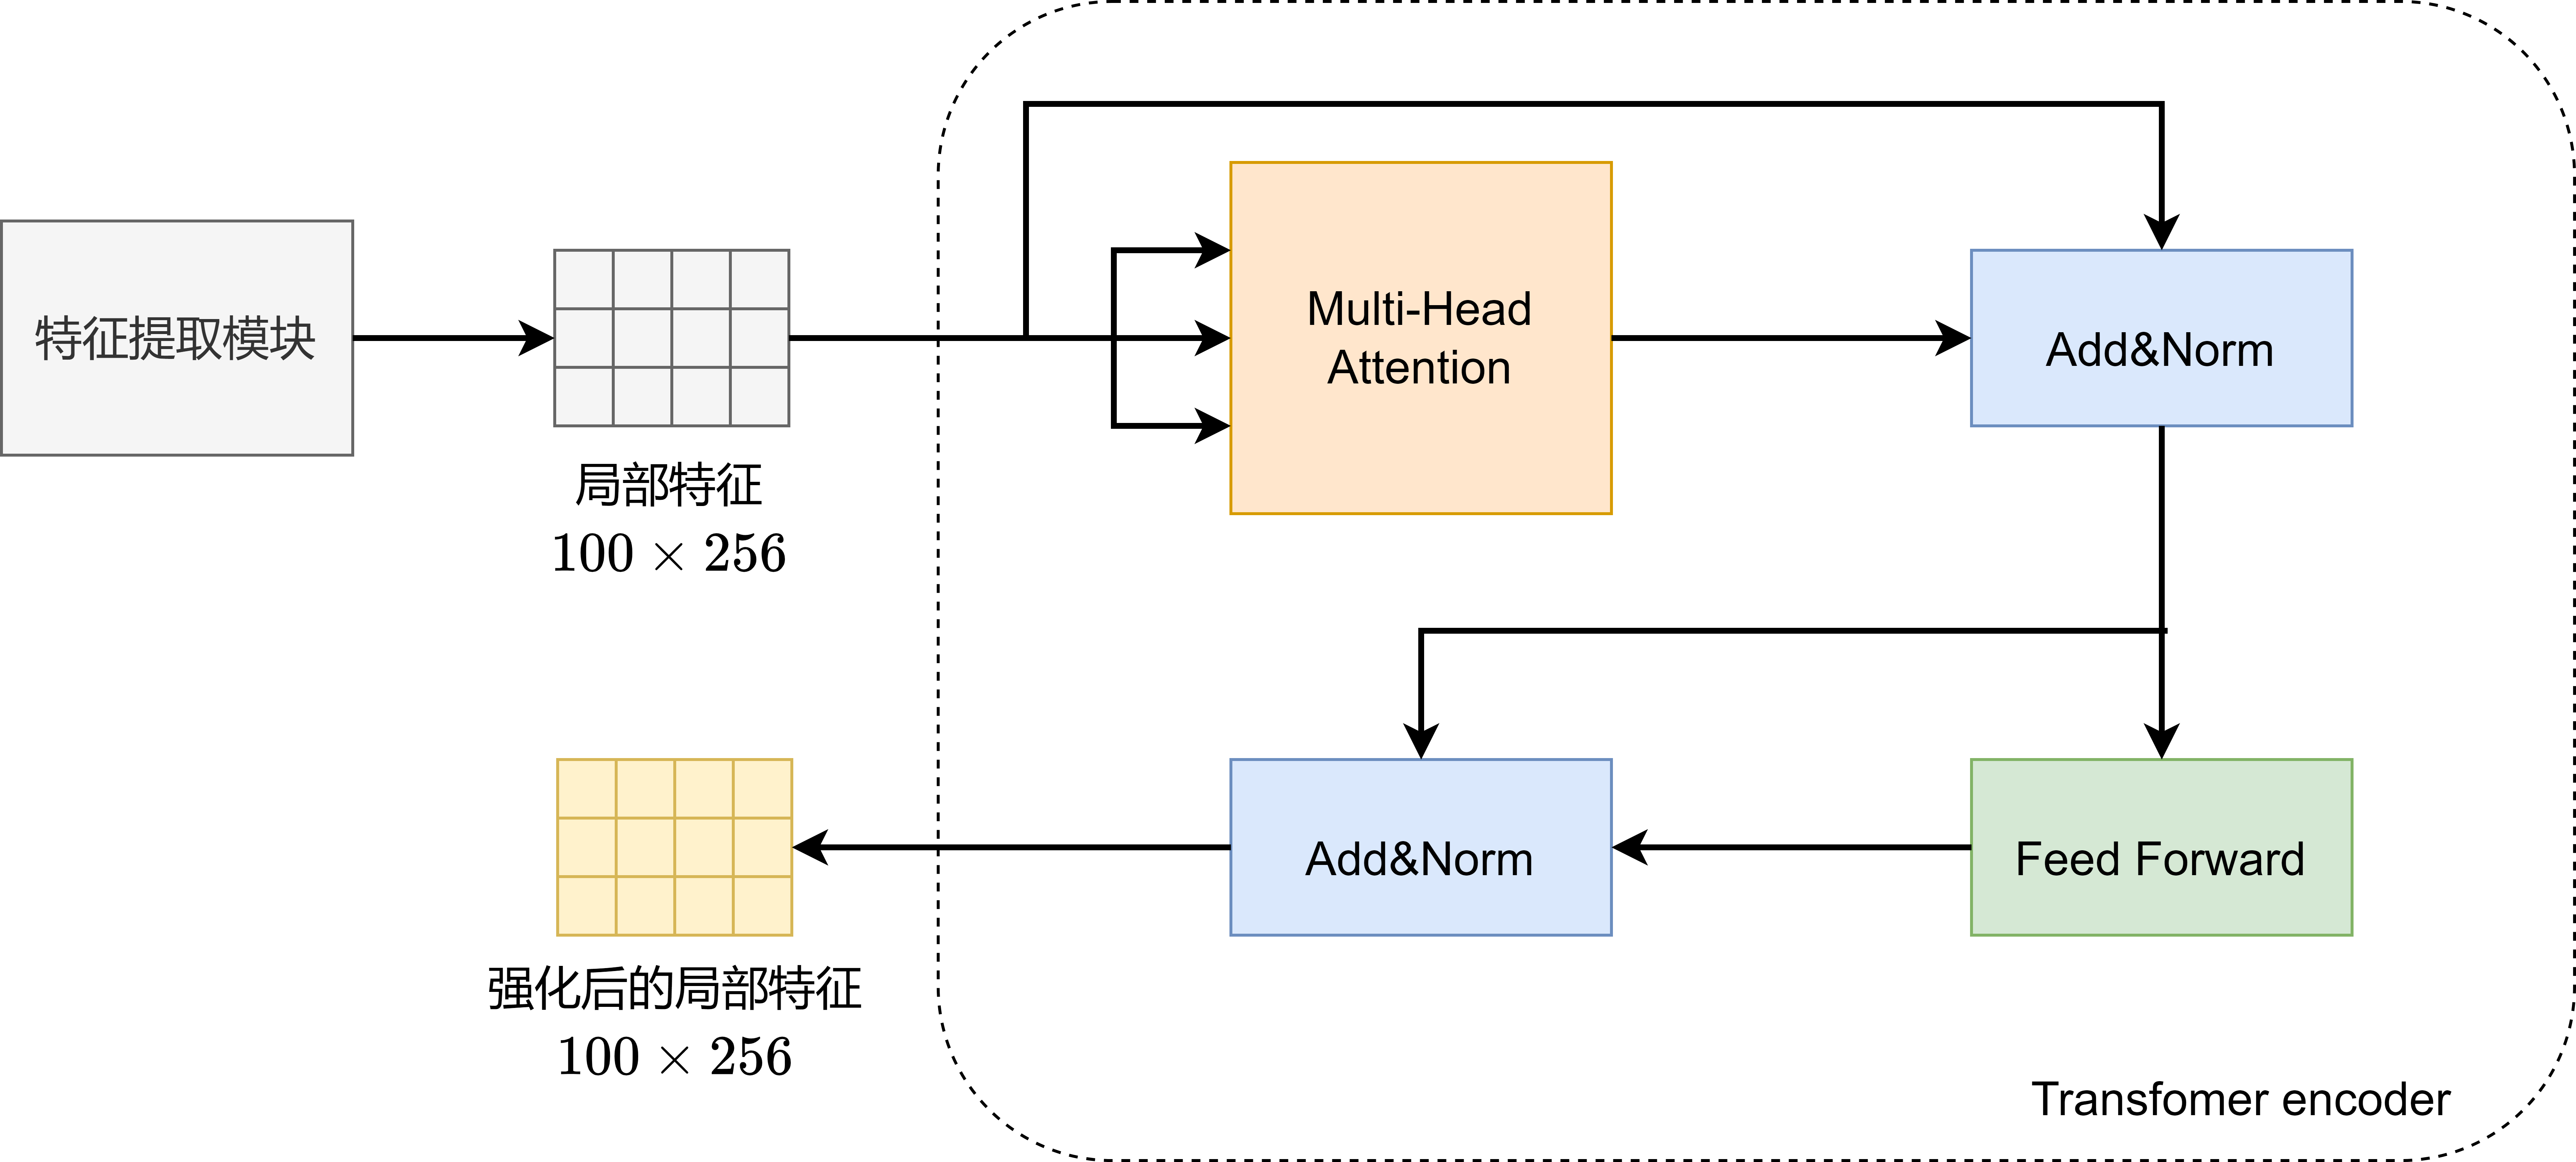
\includegraphics[scale=0.06]{Fig/encoder.png}
    \caption{\label{encoder}encoder结构图}
\end{figure}


\subsection{特征融合解码器}
特征融合的解码器decoder结构如图\ref{decoder}所示。我们将特征提取模块输出表征代理所处环境的$49 \times 256$维全局特征、表征当前导航目标的$1 \times 256$维目标特征和可学习的$1 \times 256$维目标特征进行连结,得到$51 \times 256$维的特征输入到decoder之中,在经过第一个多头自注意力层、残差连接、层归一化之后,将Transfomer encoder输出的$100 \times 256$维强化后的局部特征作为键值对、$51 \times 256$维的特征作为查询一同输入到第二个多头自注意力层之中,经过残差连接归一化层、前馈神经网络和最后一次的残差连接和层归一化后,得到$51 \times 256$维的特征,使用该特征中与$1 \times 256$维的目标特征和$1 \times 256$维的可学习的参数特征相对应位置的向量,作为表征环境中与目标相关联物体的信息,以帮助代理确定导航方向的方向特征,还有表征全局特征和局部特征共同联合的环境特征。
\begin{figure}[htbp]
    \centering
    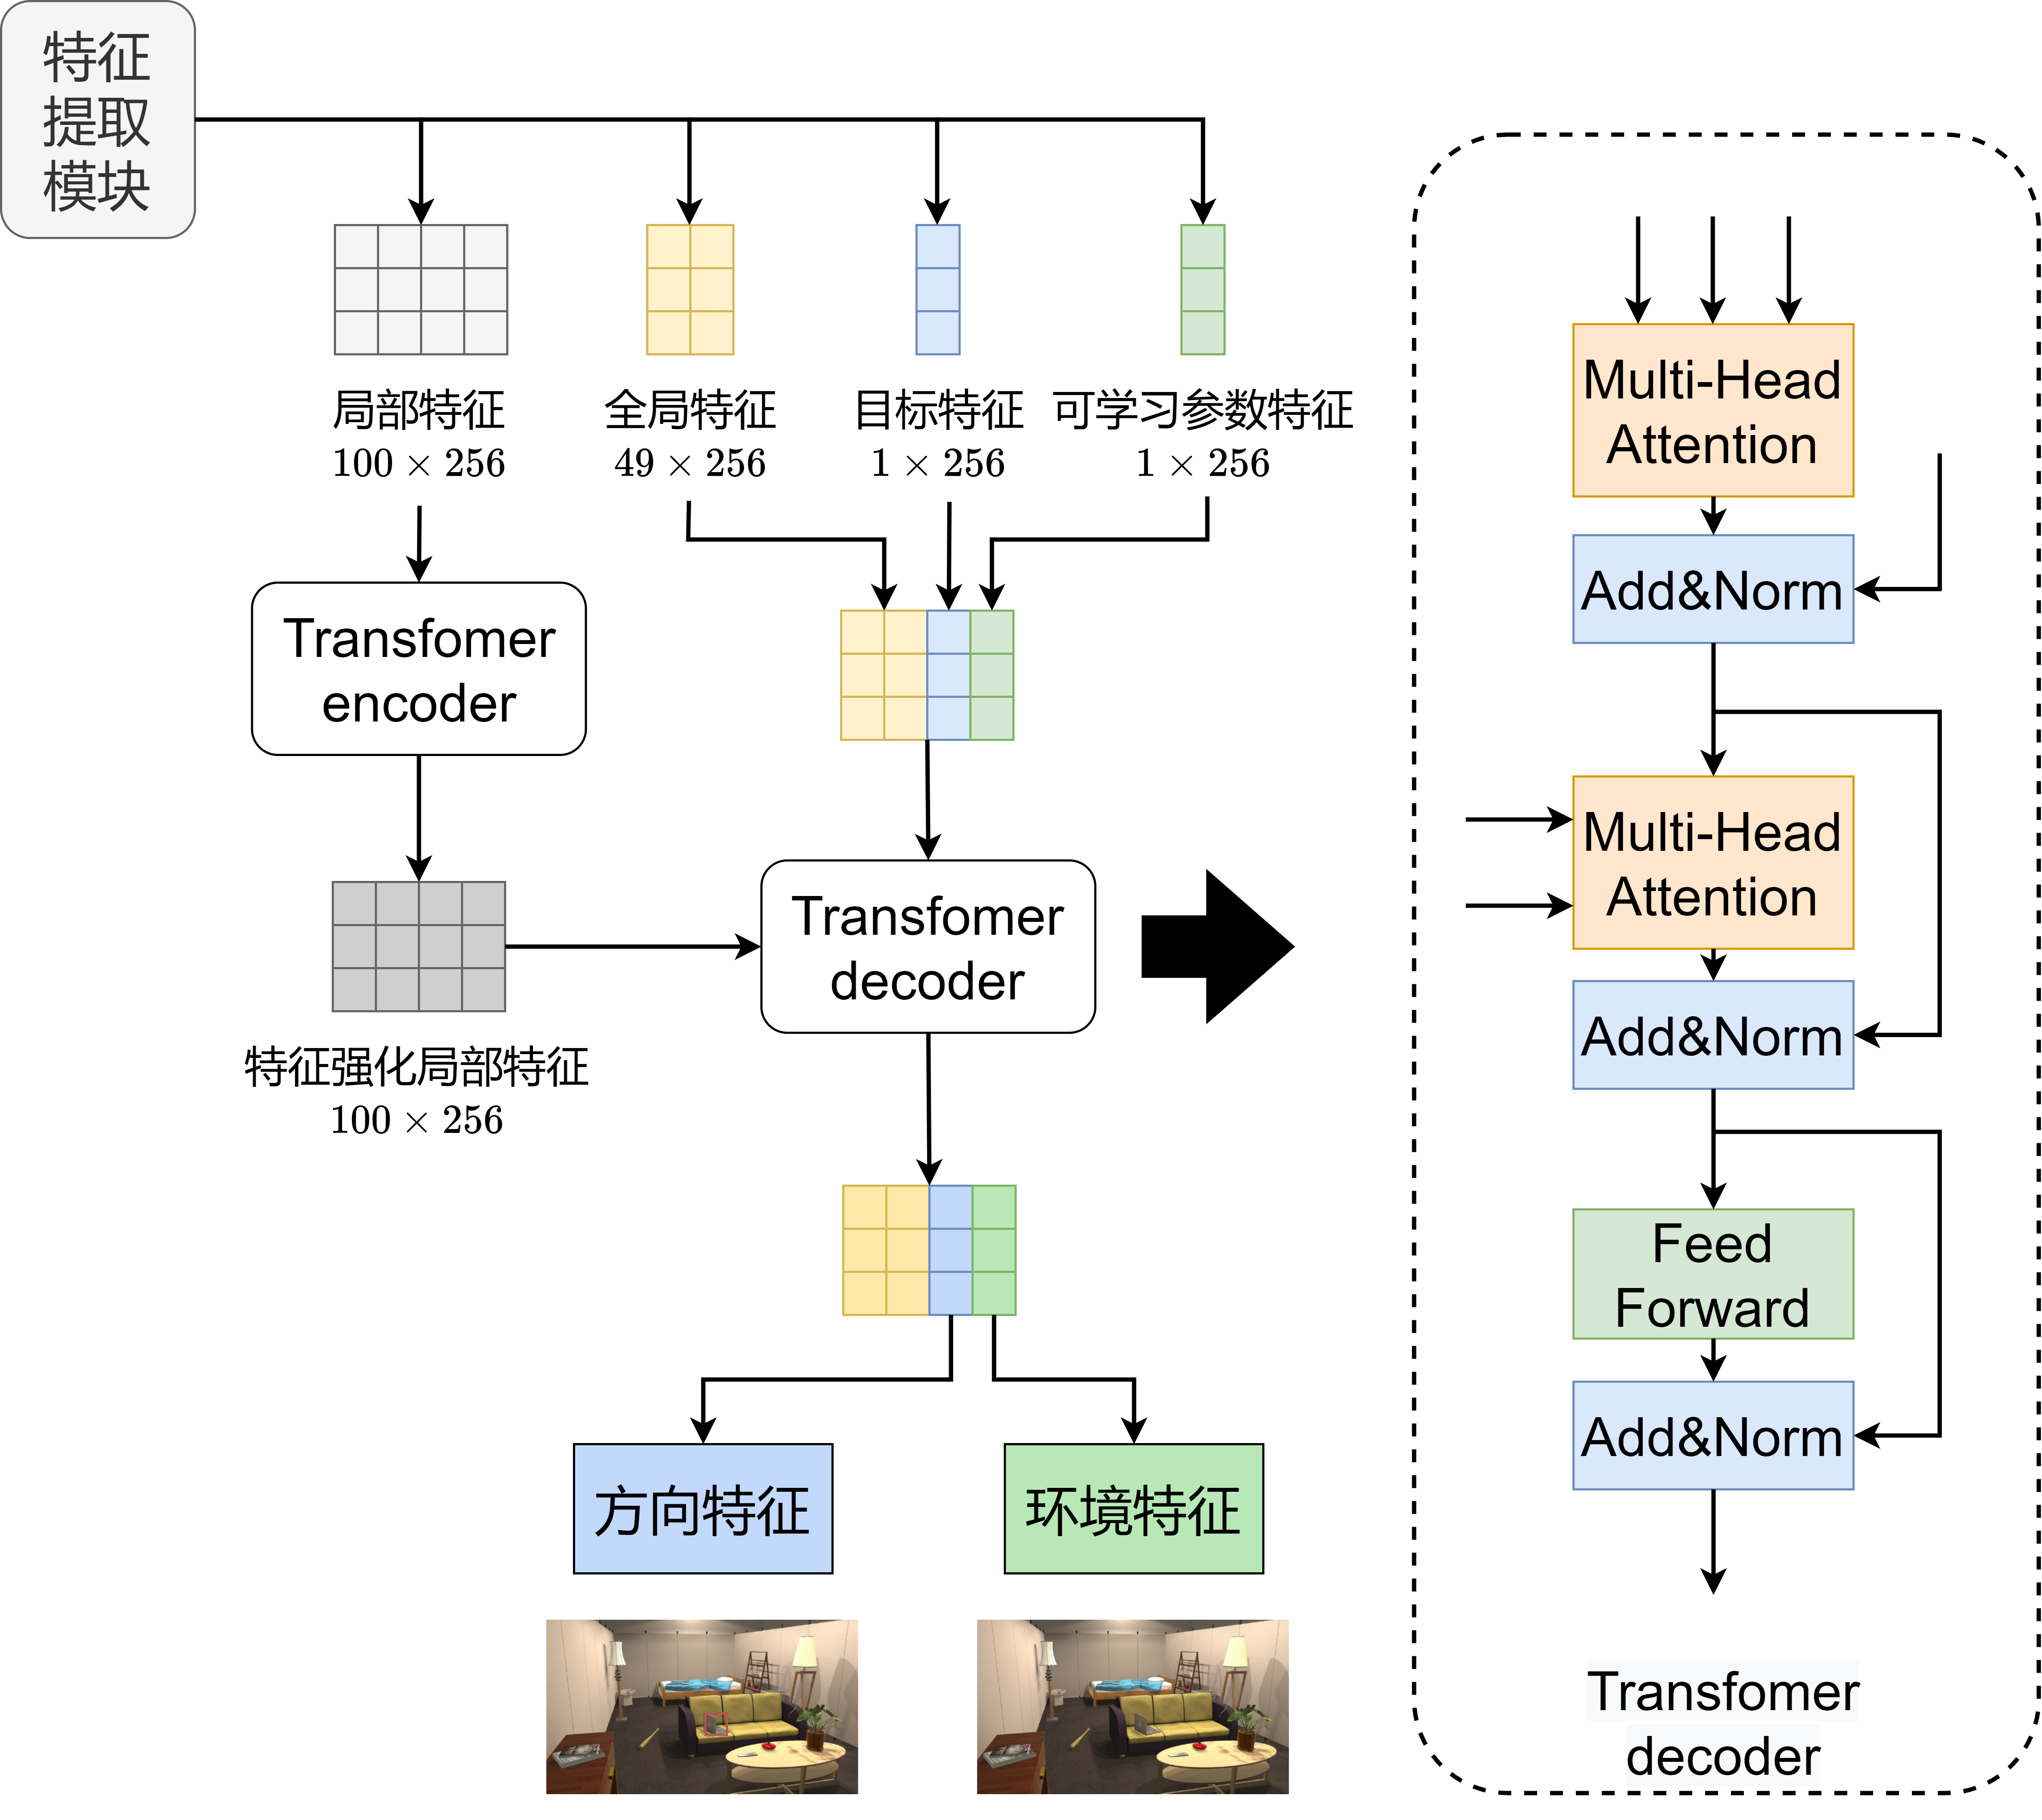
\includegraphics[scale=0.08]{Fig/decoder.png}
    \caption{\label{decoder}decoder结构图}
\end{figure}


\subsection{LSTM网络}
LSTM是一种能够有效地捕捉序列数据中的长期依赖关系的特殊循环神经网络,传统的神经网络或其他类型的RNN可能会遗忘过去的特征信息,而LSTM通过引入遗忘门、输入门和输出门从而有效地解决了这一问题,这种循环结构使得它在基于历史信息进行决策或是当任务需要依赖较长时间之前的状态时的场景中表现出色。而在机器人执行导航这种需要处理时序信息和长期依赖的任务的过程中,需要代理根据上一时刻的导航动作、方向特征和环境特征提取有用的历史信息,使用LSTM结构的网络根据以往的经验做出更精准的决策,从而达到显著提高导航系统的决策能力的目的。

通过LSTM网络输出局部未知环境下的导航动作流程如图\ref{LSTM}所示。我们将特征融合解码器输出的$1 \times 256$维方向特征、$1 \times 256$维环境特征和表示未知环境下代理所执行的$1 \times 4$维导航动作进行拼接,得到$1 \times 516$维特征向量作为双层LSTM网络的输入,最终输出$1 \times 4$维的导航动作交由运动模块所封装的导航动作执行,并且该当前时刻的导航动作在经过一个线性层后作为下一时刻的动作特征输入到LSTM网络中。
\begin{figure}[htbp]
    \centering
    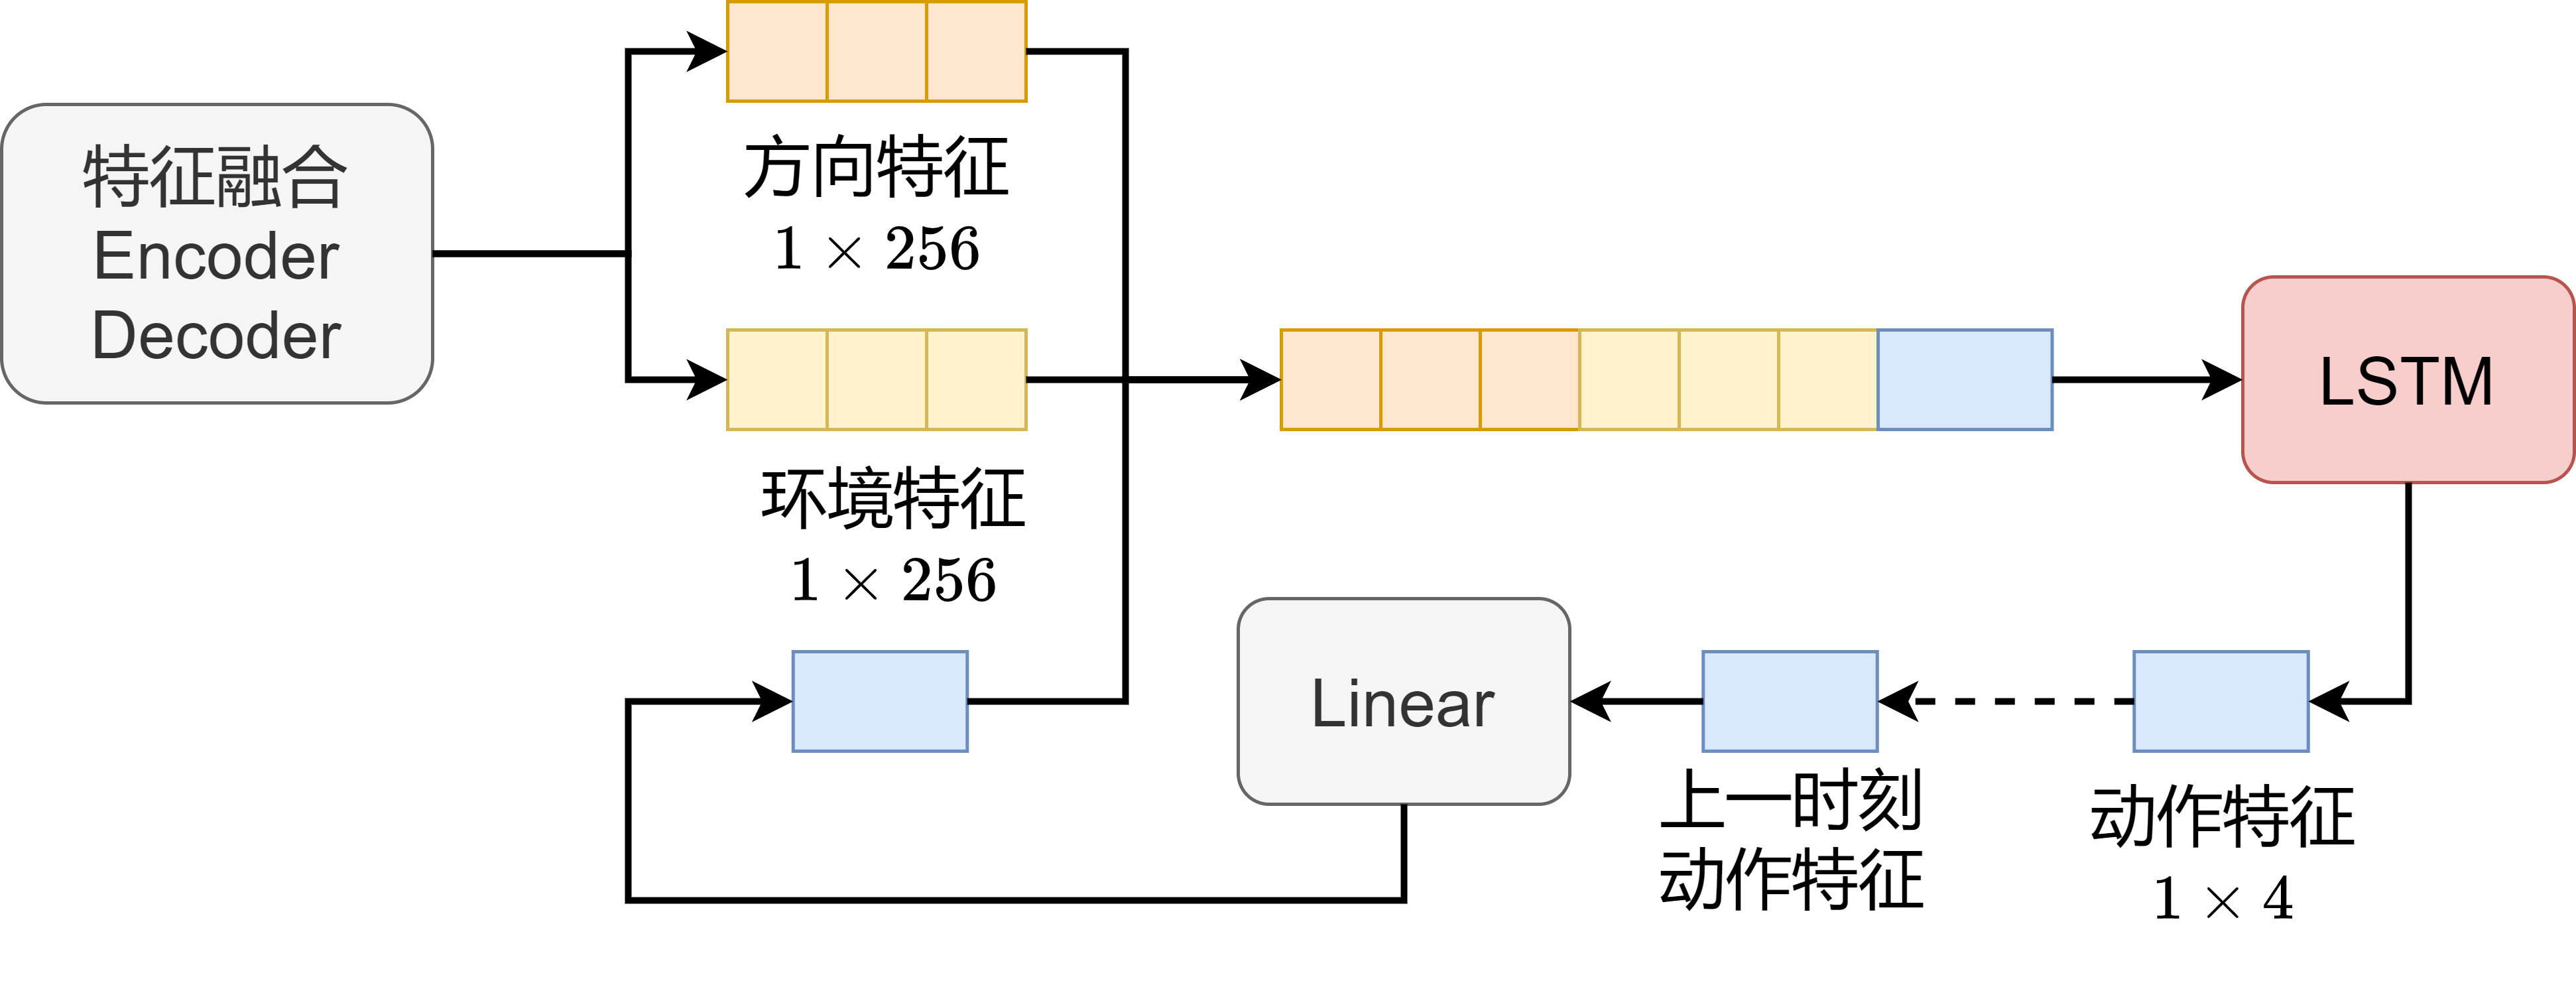
\includegraphics[scale=0.10]{Fig/LSTM.png}
    \caption{\label{LSTM}LSTM结构图}
\end{figure}


\section{运动模块}
在运动模块中,我们通过ROS的分布式通信框架来订阅目标位姿信息,依托差分驱动模型来实现机器人在环境中的移动探索。


本系统研发的移动机器人基于差速转向原理实现底盘驱动。在机械结构设计上,我们通过独立控制两侧驱动电机的转速差异来完成运动控制。当两侧驱动轮保持相同转速时机器人将保持直线行驶;当两侧转速产生差值时,根据差速传动特性机器人会以自身轴线为中心进行转向运动。基于这种原理,我们可以通过调整双轮速度参数实现不同曲率的弧线运动与精确转向定位。在制动控制方面,驱动系统可通过切断电机供电使设备实现急停功能。

具体如图\ref{motion_control}所示,底盘控制系统的工作流程包含指令下发与动态修正两个关键环节。主控制器首先将预设转速参数传输至电机驱动模块,但由于机械传动间隙、地面摩擦系数变化等客观因素,机器人车轮的实际转速值与理论设定值往往存在偏差。因此系统设计了一种闭环控制架构,驱动模块不仅需要输出PWM控制信号,还通过正交编码器实时采集电机转动参数。在10ms的采样周期内,控制模块会持续统计编码器脉冲数量并将其转换为移动距离参数进行反馈。主控单元运用运动学方程对这些原始数据进行坐标变换与轨迹拟合,最终生成毫米级精度的实时位姿信息从而保障移动平台的精准定位能力。


\begin{figure}[htbp]
    \centering
    \includegraphics[scale=0.07]{Fig/机器人底盘运动控制.png}
    \caption{\label{motion_control}机器人的运动控制方法}
\end{figure}

在控制移动机器人移动的过程中通常会受到地面摩擦阻力的影响,出现左右轮的实际转速和想要控制的速度不同的情况,导致移动机器人无法按照计划的轨迹进行移动,这时候就需要使用第二章所介绍的PID控制算法来调整小车的运动,使其能够精准的按照目标轨迹进行移动。


在移动机器人根据多特征融合网络的输出进行局部范围内的探索以期找到目标物体时,我们需要计算出每一时刻的里程计数据,并将其与订阅获取的实时里程计数据进行比较,从而计算出当前已经移动的距离,达到让机器人准确地进行移动的目的。具体来说里程计包括位姿(位置和方向角)和运动速度(线速度与角速度)两个重要的信息,它的计算过程如图\ref{motion_calculate}所示。在整个机器人运动的过程当中,假设用${p_i}$来表示在时刻$i$的位姿,图中的${p_1},{p_2}, \ldots ,{p_n}$则代表机器人的整个运动过程中的轨迹。在很短的时间内,机器人从${p_1}$运动到${p_2}$,那么我们就可以根据机器人当前的位姿${p_1}$及其左右轮的速度${V_{left}}$和${V_{right}}$,通过微积分的方法来推算机器人下一个时间步${p_2}$处的线速度、角速度及其位姿,从而计算获得完整的里程计数据。
\begin{figure}[htbp]
    \centering
    \includegraphics[scale=0.05]{Fig/移动控制.png}
    \caption{\label{motion_calculate}里程计计算}
\end{figure}

在机器人移动的三维空间中存在多个坐标系,我们构建了存在于导航环境中相对静止的全局坐标系作为机器人本体运动的参考坐标系,在任意的时刻$t$,机器人的位姿可以表示为${P_t} = \left( {{x_t},{y_t},{\theta _t}} \right)$,其中$\left( {{x_t},{y_t}} \right)$表示机器人的位姿在世界坐标系x、y平面上的投影坐标,${{\theta _t}}$表示朝向角。导航系统则基于差分轮式运动学模型进行驱动,该模型将平台的运动学状态解耦为绕瞬态旋转中心(Instantaneous Center of Rotation, ICR)的刚体转动与平移分量的合成运动,其运动可以近似视为围绕某一瞬时旋转中心,以半径r沿圆弧轨迹运动。已知左右轮的速度${V_{left}}$、${V_{right}}$及两轮间距$l$,可以通过式\eqref{myeq20}、\eqref{myeq21}和\eqref{myeq22}来计算机器人在$t$时刻的线速度$v$、角速度$\omega $以及旋转半径$r$
\begin{equation}
    v = \frac{{{v_{left}} + {v_{right}}}}{2}
    \label{myeq20}
\end{equation}
\begin{equation}
    \omega  = \frac{{{v_{right}} - {v_{left}}}}{l}\left( {{{rad} \mathord{\left/
 {\vphantom {{rad} s}} \right.
 \kern-\nulldelimiterspace} s}} \right)
    \label{myeq21}
\end{equation}
\begin{equation}
    r = \frac{v}{\omega } = \frac{l}{2} \cdot \frac{{{v_{right}} + {v_{left}}}}{{{v_{right}} - {v_{left}}}}
    \label{myeq22}
\end{equation}


在实际计算中为了推算出机器人在当前时刻的位姿,我们基于速度积分法进行计算。设在t时刻移动机器人的位姿为${P_t} = \left( {{x_{t}},{y_{t}},{\theta _{t}}} \right)$,在微笑的时间序间隔$\Delta t$内进行的运动过程可以等效为恒定速度的匀速运动,因此可以通过如下递推式\eqref{myeq23}、\eqref{myeq24}和\eqref{myeq25}计算出结果。
\begin{equation}
{\theta _{t + 1}} = {\theta _{t}} + \omega  * \Delta t
    \label{myeq23}
\end{equation}
\begin{equation}
    {x_{t + 1}} = {x_{t}} + r * \left( {\sin {\theta _{t + 1}} - \sin {\theta _{t}}} \right)
    \label{myeq24}
\end{equation}
\begin{equation}
{y_{t + 1}} = {y_{t}} - r * \left( {\cos {\theta _{t + 1}} - \cos {\theta _{t}}} \right)
    \label{myeq25}
\end{equation}
该方法能够高效、准确地计算机器人每个时刻的位姿,并依次累积得到完整的运动轨迹,为导航和路径规划提供精确的里程计数据支持。在具体的实现中我们使用面向对象的编程思想进行封装,将其用于探索未知环境。

\section{图像点云融合模块}
未知环境的目标物体导航任务要求代理要具备识别出环境中存在着的目标物体的功能。多线激光雷达具备高精度的深度测量能力,它能够提供目标的距离感知信息和三维结构,但点云数据会随着距离的变大而逐渐变得稀疏,在追踪远距离目标时效果有限。单目相机则具有高分辨率的视觉信息,能够捕捉目标的纹理、颜色和边缘特征等认知信息,但它缺乏直接的深度感知能力,同时也容易受到光照条件等环境因素的影响。相比于使用单一传感器进行目标检测,使用多线激光和单目相机的联合检测方法在各种应用场景中展现出显著的优势,能够有效降低误检和漏检率。首先图像点云融合方法能够显著提升代理对远距离目标的检测能力,即使在单目相机难以判别目标的远距离区域依旧可以通过多线激光雷达来获取准确的深度信息。此外目前的视觉言语导航方法大多仅依赖于网络模型输出的动作进行决策,使用导航至目标3米内即算完成导航任务这一笼统指标并不利于后续利用机械臂执行的下游任务的执行,这就需要多线激光提供的准确距离信息来辅助代理进行导航以完成导航至目标半米内的任务。

局部路径规划方法中的图像点云融合模块使用了第二章所介绍的YOLOV10目标检测网络、优化后的欧式点云聚类算法和多线激光单目相机联合标定方法。多线激光获取的点云在经过点云聚类之后通过外参矩阵重投影到目标检测二维图像上,并且使用IoU重叠度(Intersection over Union)来判断目标检测框中的目标物体与点云聚类结果是否匹配,当点云聚类结果与目标检测框不匹配时就会被舍弃,当结果匹配时就会被纳入结果集,并将出所选定的区域框中所有点云的均值作为该目标的距离,用以发布最终导航目标点完成完整的导航。

IoU具有非负性、不可分辨的同一性、对称性和尺度不变这类属性,这使得通过这个方法来判断两个任意形状A和B之间的相似性与它们的空间尺度无关,所以它被广泛用作计算机视觉中许多任务的评估指标,如像素级图像分割、2D和3D对象检测等。
因此,本文使用IoU度量法来衡量有限的点云聚类算法结果和目标检测算法结果之间的相似性。具体来说针对两个有限样本集合$A$和$B$,他们之间的IoU被定义为他们的交集除以他们之间的并集,如式\ref{myeq26}。
\begin{equation}
    {\rm{IoU}}\left( {A,B} \right) = \frac{{A \cap B}}{{A \cup B}} = \frac{{A \cap B}}{{\left| A \right| + \left| B \right| - A \cap B}}
    \label{myeq26}
\end{equation}

根据点云聚类和目标检测的结果可以获得两个不同的预选框,将它们通过预选框匹配算法计算他们之间的IoU度量,如算法\ref{algorithm3}。
当预选框之间的IoU低于0.5时,根据非极大值抑制准则将两者判定为独立目标;当IoU处于区间$0.4<=IoU<=0.8$时,根据置信度加权策略选取两个候选框的重叠区域作为最终检测框;对于IoU大于0.8的强相关预选框则通过最小外接矩形算法生成融合后的最终检测框,如图\ref{iou}。
\begin{algorithm}[!h]
    \caption{IoU度量算法}
    \label{algorithm3}
    \renewcommand{\algorithmicrequire}{\textbf{Input:}}
    \renewcommand{\algorithmicensure}{\textbf{Output:}}
    \renewcommand{\algorithmiccomment}[1]{\hfill $\triangleright$ #1}
    \begin{algorithmic}[1]
        \REQUIRE 检测框的四个角坐标:
        $\begin{array}{l}
            {A_1}\left( {{x_1},{y_1}} \right),{B_1}\left( {{x_2},{y_1}} \right),{C_1}\left( {{x_2},{y_2}} \right),{D_1}\left( {{x_1},{y_2}} \right)\\
            {A_1}\left( {{{x'}_1},{{y'}_1}} \right),{B_1}\left( {{{x'}_2},{{y'}_1}} \right),{C_1}\left( {{{x'}_2},{{y'}_2}} \right),{D_1}\left( {{{x'}_1},{{y'}_2}} \right)\\
            {x_1} \le {x_2},{y_2} \le {y_1},{{x'}_1} \le {{x'}_2},{{y'}_2} \le {{y'}_1}
            \end{array}$  %%input
        \ENSURE 两个预选框之间的IoU结果   %%output
        \STATE  The area of ${{\rm{B}}_{{\rm{c }}}}$:${\rm{Are}}{{\rm{a}}_{\rm{c}}} = ({x_2} - {x_1}) \times ({y_1} - {y_2})$
        \STATE  The area of ${{\rm{B}}_{{\rm{d }}}}$:${\rm{Are}}{{\rm{a}}_{\rm{d}}} = ({{x'}_2} - {{x'}_1}) \times ({{y'}_1} - {{y'}_2})$
		\STATE  The area of overlap:\\
        ${\rm{Are}}{{\rm{a}}_{{\rm{overlap}}}} = (\max ({x_2} - {{x'}_2}) - \min ({x_1},{{x'}_1})) \times (\max ({y_1} - {{y'}_1}) - \min ({y_2},{{y'}_2}))$
		\STATE  ${\rm{IoU}} = {\rm{Are}}{{\rm{a}}_{{\rm{overlap}}}}/({\rm{Are}}{{\rm{a}}_c} + {\rm{Are}}{{\rm{a}}_d} - {\rm{Are}}{{\rm{a}}_{{\rm{overlap}}}})$
    \end{algorithmic}
\end{algorithm}
\begin{figure}[htbp]
    \centering
    \includegraphics[width=0.85\textwidth]{Fig/iou.png}
    \caption{\label{iou}预选框选择策略}
\end{figure}

在经过预选框选择策略之后获得的最终边界框将用于测定目标在机器人坐标系下的位姿,如图\ref{target_pose}。通过最终边界框的中点$\left( {{u_{mid}},{v_{mid}}} \right)$和单目相机的水平视域、垂直视域,可以分别计算出目标物体与机器人$x$轴正方向的水平夹角$\phi $、目标物体与机器人$y$轴正方向的水平夹角$\varphi $。然后将投影在最终边界框中的点云距离进行均值相加以获得机器人与目标之间的距离$D$,根据$\phi $、$\varphi $和$D$可以计算出机器人坐标系下目标的位姿。
\begin{figure}[htbp]
    \centering
    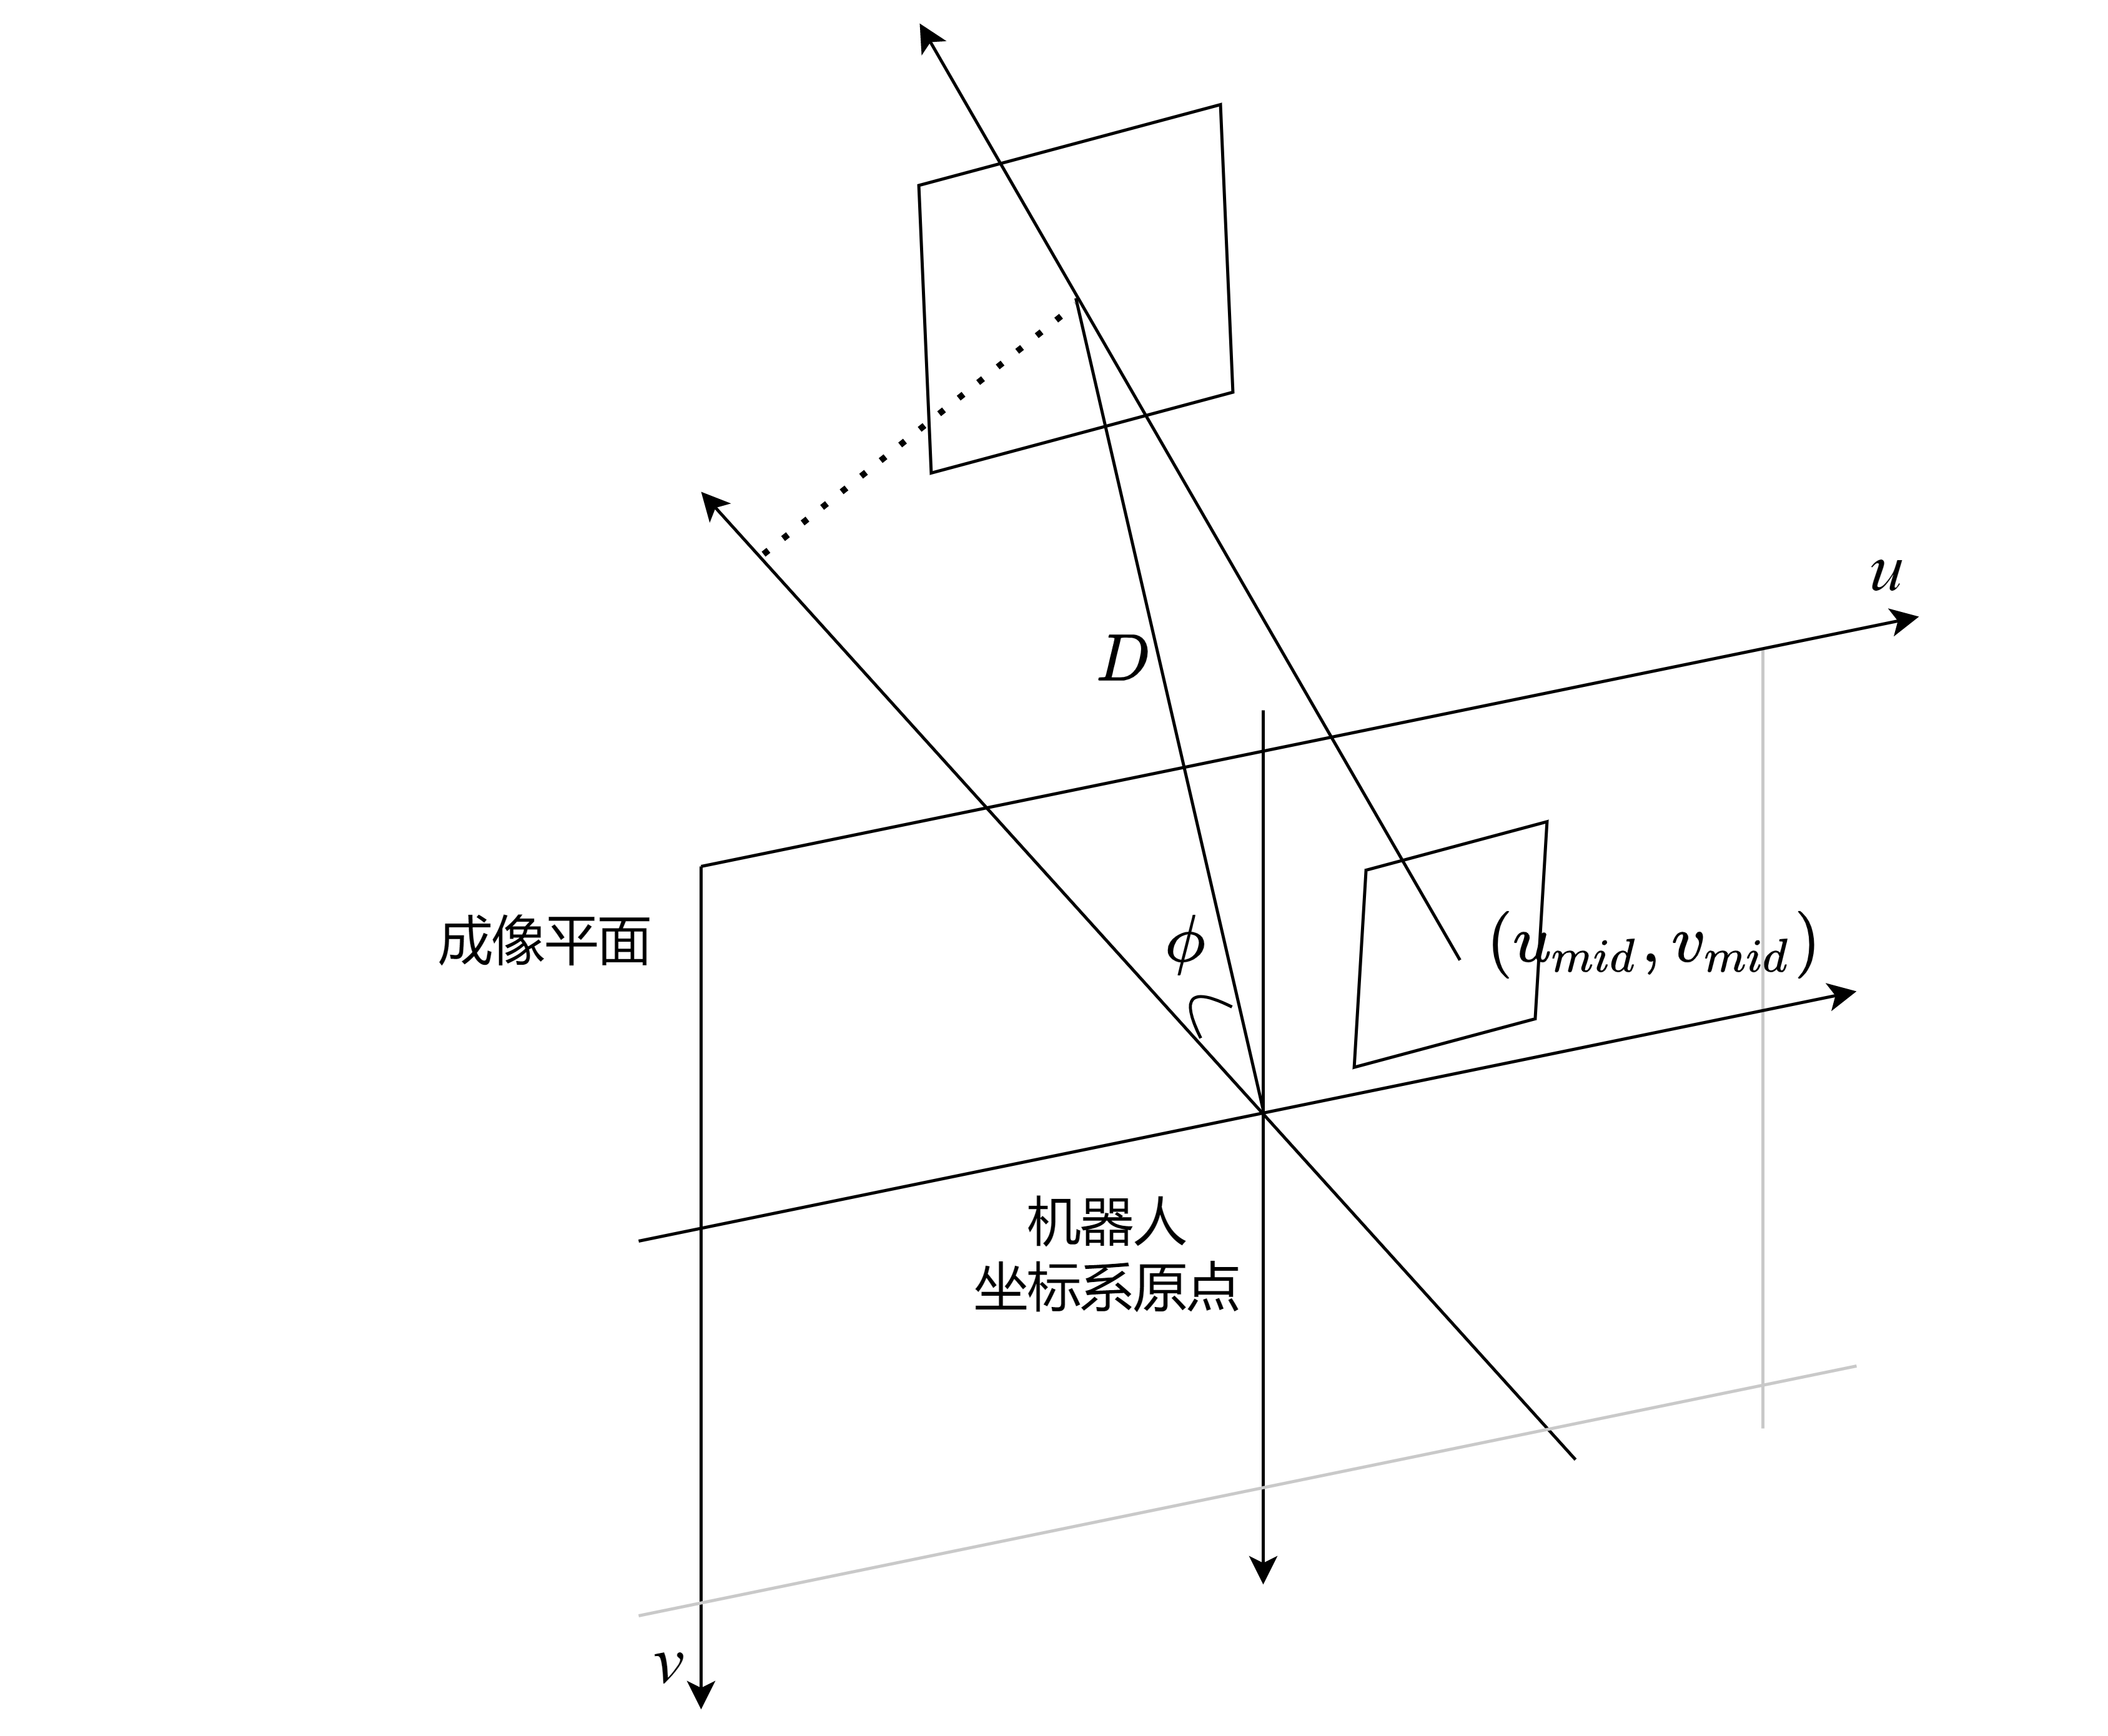
\includegraphics[scale=0.11]{Fig/目标坐标..png}
    \caption{\label{target_pose}根据平面成像与点云数据求目标位姿}
\end{figure}
最后,通过ROS框架中tf话题所提供的数据和四元组转欧拉角方法即可将机器人坐标系下的目标位姿转换成地图坐标系下的目标位姿,发布导航即可完成完整的目标物体导航任务。需要注意的是,在实验的过程中我们发现当目标物处于桌子上等不可达的位置时,移动机器人将根据AMCL规划出的路径移动到环境的边界处,这通常与环境中离目标最近的导航点不一致,因此我们在发布最后的导航点时会先检查该点是否可达,当其不可达时图像点云融合模块将输出环境中与最终目标导航点相距最近的可达点作为替代。
具体的仿真环境、现实环境和消融实验实验结果见第五章。





\section{本章小结}
本章提出了一种局部路径规划方法,该方法由特征提取模块、特征融合模块、运动模块和图像点云融合模块构成。首先根据指令中目标物体的名称,通过特征融合、特征提取网络模型输出的离散动作,依靠运动节点在局部环境中进行自主探索,同时利用视觉图像信息识别出目标物体,在视觉观察中定位目标物体后再由图像点云融合算法计算获得目标的精确位姿,转换坐标系后发布导航任务完成局部环境目标物体导航。

	\chapter{实验设计与结果分析}
本章将详细介绍我们所提出的结合全局路径规划方法和局部路径规划方法的LVL-Nav方法在仿真环境和真实环境下的实验评估结果,包括在仿真环境中不同方法的对比实验来验证本文所提出方法的有效性、针对提出方法的各关键组件进行消融实验分析各个组件的作用和在真实环境中进行目标物体导航的实验。


\section{仿真环境实验设计与评估}
\subsection{数据集}
在仿真实验中,我们使用Gazebo中的离线数据集来进行导航实验以测试我们所提出方法的有效性。Gazebo是一个广泛用于机器人导航控制研究的强大开源仿真环境,它提供了一个高质量的物理引擎来模拟机器人在复杂的环境中的运动、感知、认知和交互,如表\ref{Gazebo与其他仿真环境对比}所示,其中可导航指的是导航代理可以在仿真环境中进行自主移动以探索不同的空间环境;可交互指的是可以手动调整环境中物体的摆放位置或是添加目标物体;物体状态表示环境中的物体会随着时间轴而发生变化,比如钟表会不停地走;动态照明是指随环境中的光源可以动态进行调整,且环境中的物体会随着光源位置的变化而产生不同的阴影;3D资源库指的该仿真环境提供可以添加在环境中不同物体的社区资源;真实对应指的是所使用的仿真世界不是随机生成而是与真实环境一一对应还原的。
相较于其他仿真环境,Gazebo能够提供更全面丰富的可视化系统和导航功能。
\begin{table}
    \caption{\label{Gazebo与其他仿真环境对比}Gazebo与其他仿真环境对比}
    \centering
    \small
    \begin{tabular}{ccccccc}
        \hline
        仿真环境 & 可导航 & 可交互 & 物体状态 & 动态照明 & 3D资源库 & 真实对应 \tabularnewline 
        \hline 
        Gazebo & \checkmark & \checkmark & \checkmark & \checkmark & \checkmark & \checkmark \tabularnewline
        iGibson & \checkmark & \checkmark &  &  &  &  \tabularnewline
        Matterport3D & \checkmark &  &  &  &  &  \tabularnewline
        Minos & \checkmark &  &  &  &  &  \tabularnewline
        Habitat & \checkmark &  &  &  &  &  \tabularnewline
        \hline 
\end{tabular}
\end{table}

在实验的过程中我们使用了类民住房、类酒店、类工厂3种具有不同尺度不同特征的场景,每种类型的场景中都有10个不同样式的环境,环境中共存在有1000多个物体,且每个环境都有120多条自然语言导航指令用于导航测试。自然语言导航指令有单目标、三目标和五目标三种不同的形式,每个环境之下的每种指令都有40多条用于测试导航方法的性能。本文所设计的LVL-Nav方法可以选择22个不同的物体作为导航目标,包括手提电脑、鼠标、花盆、台灯、沙发等室内常见家具。

在全局路径规划过程中,我们通过搭载在移动机器人上的十六线激光雷达在各仿真环境中构建栅格地图,根据所建的栅格地图设置通路中的导航点,并通过ROS导航节点进行导航,记录导航时间构建用邻接矩阵的形式表示的拓扑图。此外,我们获取环境中已经设置的所有导航点的四个方向的位姿信息和对应的视觉观察图像作为全局路径规划导航的依据,用于多模态融合网络模块匹配导航点和目标和执行后续的导航任务。

在局部路径规划过程中,需要获取仿真环境中的特征信息来训练特征提取、特征融合网络模型。具体而言,我们将每个环境都进行网格化,每个网格代表移动机器人能在环境中进行移动的离散动作步,我们将每个到导航点所获得视觉观察送入到预训练的ResNet18网络中提取特征,融合将该导航点的坐标和该点的特征作为键值对进行存储,除此之外,我们还将环境中所存在的所有目标物体的位姿、名称和可以看到该目标物体的导航点作为键值对进行存储。最终获得由导航点、目标物体和最佳动作共同构成的预训练数据集。在训练时,模型首先获得的目标物体名称和当前导航点位姿,然后它会根据导航点所对应的特征输出一个导航动作并和最佳动作计算交叉熵。在不同环境的测试过程中,我们随机给定不同的初始位姿和导航指令。



\subsection{实验参数}%机器人运动参数、多模态融合模块(训练参数) 特征提取、特征融合
在仿真环境中,我们所搭建的移动机器人的运动参数如下表\ref{robotparameter}所示。
\begin{table}
    \caption{\label{robotparameter}机器人运动参数}
    \centering
    \small
    \begin{tabular}{cccccc}
        \hline
        最大线速度 & 最大角速度 & 最大线加速度 & 最大角加速度 & 线速度分辨率 & 角速度分辨率 \tabularnewline 
        \hline 
        0.6${m \mathord{\left/
 {\vphantom {m s}} \right.
 \kern-\nulldelimiterspace} s}$ & 25${^\circ  \mathord{\left/
 {\vphantom {^\circ  s}} \right.
 \kern-\nulldelimiterspace} s}$ &  0.2${{m \mathord{\left/
 {\vphantom {m s}} \right.
 \kern-\nulldelimiterspace} s}^2}$ & 30${{^\circ  \mathord{\left/
 {\vphantom {^\circ  s}} \right.
 \kern-\nulldelimiterspace} s}^2}$  &  0.01${m \mathord{\left/
 {\vphantom {m s}} \right.
 \kern-\nulldelimiterspace} s}$ &  1${^\circ  \mathord{\left/
 {\vphantom {^\circ  s}} \right.
 \kern-\nulldelimiterspace} s}$ \tabularnewline
        \hline 
    \end{tabular}
\end{table}

全局路径规划中的多模态融合网络通过在Interiornet数据集筛选后的20w个数据集进行训练,使用Adam优化器以${10^{ - 4}}$的学习率更新CLIDP网络,我们使用20个异步代理训练5000次episode,每次的batch\_size为128,且每100次保存一次模型数据和精度,然后将得到的模型在划分的验证集里测试精度,最终选取精度最高的模型作为后续导航所使用的模型。
局部路径规划中的特征提取、特征融合模块通过预训练的模型权重进行初始化,使用Adam优化器以${10^{ - 5}}$的学习率更新模型,我们使用20个异步代理训练300万次episode,每10万次保存一次模型数据和精度,然后将得到的30个模型在验证集里测试精度,最终选取精度最高的模型作为后续导航所使用的模型。




\subsection{实验设备}
所有的仿真实验是在笔记本电脑上进行的,模型的训练则是在服务器上进行的,它们的的主要配置参数如表所示\ref{platformconfig}。我们使用双系统的方式在笔记本电脑上安装Ubuntu20.04并搭建ROS所依赖的相关环境,使用vSCode作为代码编辑、环境配置管理和远程连接工具。在服务器上则使用docker容器进行模型训练环境的配置和依赖的安装。
\begin{table}
    \caption{\label{platformconfig}实验平台配置参数}
    \centering
    \small
    \begin{tabular}{ccc}
        \hline
        软硬件 & 服务器配置 & 笔记本电脑配置 \tabularnewline 
        \hline 
        GPU & NVIDIA GeForce RTX 2080Ti × 3 & NVIDIA GeForce RTX 3050Ti \tabularnewline
        CPU & Intel Xeon E5-2620 v4 (32)@3 & AMD Ryzen 9 5900HS \tabularnewline
        内存 & 128GB & 16GB \tabularnewline
        存储 & 4T & 1T \tabularnewline
        操作系统 & Ubuntu18.04 & Ubuntu18.04 \tabularnewline
        开发环境 & Python3.8+Pytorch1.9 & Python3.8+Pytorch1.9 \tabularnewline
        \hline 
    \end{tabular}
\end{table}








\subsection{评价指标}
本文通过导航成功率(SR)、导航路径匹配度(PMD)和导航效率(SPL)三个方面来评估导航方法的综合性能,SR衡量导航的有效性,MD衡量导航符合指令要求的程度,SPL衡量导航效率,其具体表达公式如下。
\begin{enumerate}[topsep = 0 pt, itemsep= 0 pt, parsep=0pt, partopsep=0pt, leftmargin=44pt, itemindent=0pt, labelsep=6pt, label=(\arabic*)]
    \item 	\textbf{成功率(Success Rate, SR)}。成功率指移动机器人根据自然语言指令进行导航的过程中,成功完成导航所占的比例,取值范围从0到1。
    \begin{equation}
        SR = \frac{1}{N}\sum\limits_{n = 1}^N {{S_n}} 
        \label{myeq51}
    \end{equation}
    其中$N$表示导航总次数,${S_n}$表示执行第n次导航的指标,导航成功时值为1,导航失败时值为0。
    \item	\textbf{路径匹配度(Path Matching Degree, PMD)}路径匹配度指移动机器人根据自然语言指令进行导航的过程中,依次经过的目标与指令要求的目标相匹配所占的比例,取值范围从0到1。
    \begin{equation}
        PMD = \frac{1}{{N \cdot M}}\sum\limits_{n = 1}^N {\left( {\sum\limits_{m = 1}^M {{a_{nm}}} } \right)} 
        \label{myeq53}
    \end{equation}
    其中$M$表示导航指令中存在的目标个数,$a_{nm}$表示导航子目表匹配指标,导航点匹配时值为1,导航点不匹配时值为0。
    \item	\textbf{成功路径长度加权比率(Success weighted by Path Length, SPL)}。成功路径长度加权比率指移动机器人根据自然语言指令进行导航的过程中,根据实际执行路径和最优路径的关系从0到1取值,当实际执行路径与导航最优路径越接近则取值越高,代表导航的效率越高。
    \begin{equation}
SPL = \frac{1}{N}\sum\limits_{n = 1}^N {\left( {{S_n} \cdot \left( {\frac{{{T_n}}}{{{t_n}}}} \right)} \right)} 
        \label{myeq53}
    \end{equation}
    其中$T_{n}$表示完成第n次导航时所需的最短时间,$t_{n}$表示完成第n次导航时的实际耗时。
\end{enumerate}






\subsection{对比实验}

\subsubsection{对比方法}
\begin{enumerate}[topsep = 0 pt, itemsep= 0 pt, parsep=0pt, partopsep=0pt, leftmargin=44pt, itemindent=0pt, labelsep=6pt, label=(\arabic*)]
    \item 	Random Policy:随机策略模型的代理在随机的时间步中,根据平均的概率分布去选择动作空间中的动作进行执行,或是直接在环境中停止以结束导航任务。
    \item	Baseline:基准导航策略直接将局部路径规划中的特征提取得到的局部、全局和目标特征直接送入LSTM网络进行离散动作推理。用于对比验证本文所提出方法中特征融合模块的作用。
    \item   CLIP:CLIP基于对比学习的方法提出了一种多模态融合的网络结构,通过有效地将图像和文本信息结合在一起来提供更强的跨模态理解能力,克服了传统模型依赖单一数据源的缺陷,使移动机器人能够理解环境中的目标物体和语义信息以指导导航任务的执行。
    \item   EONS:EONS借助ROS框架提出了一种有效的目标导航策略。首先对常见的室内物体进行语义关联分析,利用Mask R-CNN和残差连接网络建立物体语义关联模型,通过ROB-SLAM系统方法构建了一个高可用性的环境图,在移动机器人导航的过程中寻找可达的最优路径以完成导航。
    \item	ViNG:与传统的基于地图或几何推理的导航方法不同,ViNG提出了一种创新的视觉语言导航方法,通过学习如何从视觉目标图像中推断导航策略和先前观察到的数据构建环境的拓扑图,通过导航点建议(Waypoint Proposal)、拓扑图剪枝(Graph Pruning)和负挖掘(Negative Mining)多种核心策略,使机器人能够根据目标图像和环境拓扑图在现实世界环境中实现高效率的自主导航。
    \item	LM-Nav:LM-Nav通过三个大型预训练模型协同合作,完成了移动机器人根据自然语言指令进行导航的全部流程,包括负责将用户输入的自然语言指令转化为具有顺序的目标序列大语言模型GPT3、负责将目标序列与环境地图中的节点进行特征关联以建立具有先后导航顺序的导航点视觉语言模型(VLM)和负责构建环境拓扑图并利用凸优化技术规划从起点到终点最优路径的视觉导航模型(VNM)。
    \item	LVL-Nav(Ours):提出了一种多模态融合的导航方法,将导航过程拆分成全局和局部路径规划两个部分。通过引入深度信息优化传统的视觉语言模型,提出一种方位优化算法筛选不符合方位条件的冗余导航点,结合导航点规划算法进一步提高全局路径规划中导航点的正确率,再通过特征提取、融合网络在局部未知环境中进行探索,最后由图像点云融合模块完成目标物体导航任务。
	
\end{enumerate}

\subsubsection{对比结果}
在和近三年流行方法的对比试验如表\ref{cmpresult}所示。本文所提出的方法的导航指标在五目标的导航测试指令中的成功率SR(77.4\%)、路径匹配度PDM(77.4\%)和成功路径长度加权比率(62.1\%)三个指标中的性能表现都是最好的。在与五目标指令的基准模型的对比中,本文所提出方法的成功率SR(+22.9\%)、路径匹配度PDM(+23.5\%)和成功路径长度加权比率(+22.6\%)三个指标都大大超过了基准模型。在五目标指令实验中与当前表现最好的LM-Nav模型相比,本文的方法在成功率SR(+1.9\%)、路径匹配度PDM(+3.5\%)和成功路径长度加权比率(+8.7\%)三个指标上也都有所提升,这是因为我们在全局路径规划中通过引入深度信息优化多模态融合网络,提高模型在光线条件变化大的室内的鲁棒性,提出了一种方位优化法,结合指令中提供的方位信息与移动机器人的实时位姿,筛选不符合方位条件的冗余导航点,再通过导航点规划算法进一步提高全局路径规划所生成导航点的正确率,然后在局部路径规划中我们设计了一种特征提取、融合网络能够有效地在局部未知环境中进行探索,设计并实现了一种单目相机和多线激光传感器融合的局部导航方法,以完成导航至目标半米内的闭环任务,这表明了我们所提出方法的有效性。
\begin{table}[]
\caption{\label{cmpresult}实验定量结果对比}
\centering
    \begin{tabular}{c|ccc|ccc|ccc}
    \hline
    \multirow{2}{*}{Methhod} & \multicolumn{3}{c|}{I=1} & \multicolumn{3}{c|}{I=3} & \multicolumn{3}{c}{I=5}                 \\ \cline{2-10} 
                             & SR     & PMD    & SPL    & SR     & PMD    & SPL    & SR   & PMD  & SPL                       \\ \hline
    Ramdom                   & 6      & 6      & 3.9    & 0      & 0      & 0      & 0    & 0    & 0                         \\
    CLIP                     & 66.2   & 66.2   & 65.3   & 42.2   & 43.7   & 64.9   & 32.7 & 36.5 & 60.6                      \\
    Baseline                 & 73.1   & 73.1   & 48.3   & 67.4   & 69.5   & 45.8   & 51.8 & 53.9 & 39.5                      \\
    EONS                     & 78.5   & 78.5   & 31.7   & 75.0   & 76.8   & 29.4   & 64.1 & 65.5 & 26.2                      \\
    ViNG                     & 82.6   & 82.6   & 63.3   & 79.3   & 78.9   & 62.2   & 70.7 & 71.1 & 59.0                      \\
    LM-Nav                   & 85.3   & 85.3   & 57.6   & 79.4   & 77.1   & 54.9   & 72.8 & 73.9 & 53.4                      \\ \hline
    \textbf{Ours}            & \textbf{88.4}   & \textbf{88.4}   & \textbf{66.7}   & \textbf{82.3}   & \textbf{82.9}   & \textbf{65.2}   & \textbf{74.7} & \textbf{77.4} & \textbf{62.1} \\ \hline
    \end{tabular}
    \label{cmpresult}
    \end{table}


相比于我们所提出的方法,CLIP将图像和文本嵌入同一空间中来判断导航目标,但在动态变化的室内环境中容易发生物体移动、光线变化等情况,或是环境中的多个位置都存在相同的目标物体时,该模型缺乏足够的动态适应和区分不同方向正确目标的能力,无法有效地将导航点与目标做出正确的匹配从而导致导航失败,这导致该方法在导航成功率方面的指标表现不佳。

EONS借助构建的语义关联模型在环境中通过直接寻找目标物体或是与目标最相关联的物体从而引导代理执行导航任务。但这种方法依赖于训练过程中环境物体之间的固定关联信息,在静态的环境中表现较为出色,但对于存在多种移动物体的动态环境中,这种目标导航策略无法及时更新目标位置和状态,从而引发导航的错误。除此之外,当EONS在导航过程中未能第一时间观察到目标时,会根据关联模型寻找关联性最强的物体进行探索,这种探索策略占用了大部分的导航时间,导致该方法在导航效率方面的指标表现不佳。

ViNG通过结合视觉目标学习和构建环境拓扑图实现了基于视觉的目标导航,因此在导航效率指标上取得了不错的结果,但是它过度依赖于视觉目标的识别的定位,在很有可能出现遮挡或曝光、欠爆的复杂的室内环境中容易导致目标识别失败,模型无法正确的指导代理进行有效的探索从而导致导航任务的失败。这导致该方法在导航成功率方面的指标表现不佳。

LM-Nav通过大语言模型有效的解析导航任务,利用大量导航数据训练视觉语言模型和视觉导航模型,在多种复杂环境中指导代理生成正确的导航动作,这种联合多种大模型在环境中执行导航任务的方式具有一定的有效性,但这种导航方法在执行任务的过程中依赖于模型的推理速度,等待各种大模型响应的时间占据了部分的导航时间,因此它的导航效率并不高。

LM-Nav在实验中取得了次优的结果,该方法与我们所提出的LVL-Nav导航方法在根据不同指令执行导航任务时的轨迹结果如图\ref{LM-NavcmpLVL-Nav}所示,其中$S$表示随机初始化的移动机器人起点,标号$1,2,...,5$分别表示算法根据指令所执行经过的子目表导航点,$D$表示本文提出方法中局部路径规划获得的导航终点。具体来说,在类家庭仿真环境$a)$中LM-Nav方法无法正确匹配到曝光状态下的沙发,引导移动机器人移动至错误的导航点,而本文提出的LVL-Nav则通过引入深度信息提高模型在曝光或欠爆的室内环境中的鲁棒性,在全局路径规划中正确地匹配到了曝光状态下的沙发;在$b)$、$c)$中LM-Nav方法无法正确避免环境中所存在的其他相似物体影响导航的规划,当指令要求移动到路障或椅子旁时,将移动机器人引导至错误的导航点,而本文所提出的方位优化法能够结合指令中提供的方位信息与移动机器人的实时位姿,筛选不符合方位条件的冗余导航点,在全局路径规划中正确地匹配指令所指方向的目标。图\ref{CMP}和表\ref{cmpresult}统计的结果表明,本文所提出的方法不依赖于导航点的初始化,能够在动态变化复杂环境中指导代理正确地匹配导航点,在局部路径规划部分高效执行探索动作并可靠地完成导航至目标半米内的闭环任务。


\begin{figure}[htbp]
    \centering
    %\includegraphics[width=3in]{fig5}
    \subfloat[类家庭仿真环境下的导航]{
            \includegraphics[width=0.9\textwidth]{Fig/cmp-small-house.drawio.png}}\\
    \subfloat[类工厂仿真环境下的导航]{
            \includegraphics[width=0.9\textwidth]{Fig/cmp-factory.png}}\\
    \subfloat[类医院仿真环境下的导航]{
            \includegraphics[width=0.9\textwidth]{Fig/cmp-hospital.png}}
    \caption{LM-Nav和LVL-Nav路径对比图}
    \label{LM-NavcmpLVL-Nav}
\end{figure}
    
在对比实验的过程中,我们把本文全局路径规划中的多模态融合方法和LM-Nav方法在训练过程中每200个epoch保存一次的模型在验证集上测试精度。如图\ref{curvecmp}所示,将两种方法在测试集上的成功率SR进行对比,可以发现本文提出的方法在经过足够的训练后的表现优于LM-Nav。本方法的模型中添加了深度图特征提取架构,学习的速度会更慢,我们的方法在第1800个epoch时的SR只有53.3\%,而LM-Nav方法则达到了66.9\%(+13.6\%)。此外,我们的方法在训练的过程中收敛更慢,在第2400个epoch时LM-Nav方法基本收敛到精度最高值,而我们的方法则在3400个epoch时候才基本收敛到精度最高值。另一方面,我们的方法在3400次epoch后得到的精度最高值74.7\%(+1.9\%)比LM-Nav方法的精度最高值72.8\%在测试集上的表现会更好,这得益于我们提出的多模态融合网络框架能够结合深度特征信息归纳表征视觉观察和目标物体文本特征,能够在复杂光照条件下正确通过利用深度信息进行图像-文本匹配,从而有效地提升导航的成功率。

\begin{figure}[htbp]
    \centering
    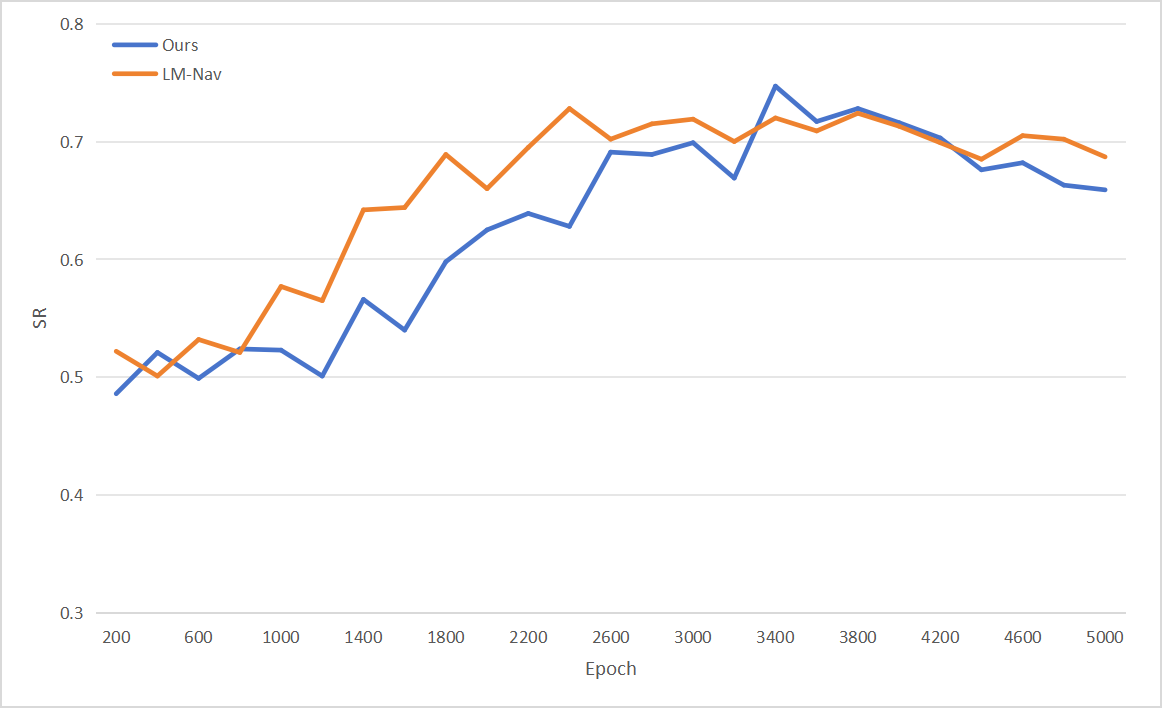
\includegraphics[scale=0.70]{Fig/curvecmp.png}
    \caption{\label{curvecmp}导航指标变化图}
\end{figure}


\subsection{消融实验}

了逐步验证本文所提出的多模态融合网络、导航点规划、方位优化和局部路径规划算法的有效性,我们对上述各关键模块进行仿真消融实验。我们在仿真环境下进行的消融实验中依次添加多模态融合模块、导航点规划算法、方位优化算法、局部路径规划算法来测试各个模块对于指导代理进行高效且正确地导航的有效性,根据他们分别执行基于自然语言指令后记录的评价指标结果如表\ref{Ablationtable}所示,我们分析了各模块的作用。
\begin{enumerate}[topsep = 0 pt, itemsep= 0 pt, parsep=0pt, partopsep=0pt, leftmargin=44pt, itemindent=0pt, labelsep=6pt, label=(\arabic*)]
    \item 	多模态融合模块:我们直接使用多模态融合网络进行指令目标与导航点之间的匹配,并将匹配的结果直接发布至/move\_base\_simple话题之中交由ROS导航节点执行导航。实验结果表明在单目标指令中成功率SR(-22.2\%)成功路径长度加权比率(-1.4\%),在五目标指令中成功率SR(-25.1\%)、路径匹配度PDM(-25.5\%)和成功路径长度加权比率(-2.8\%),由于缺失了导航点规划算法所引入的加权最短距离算法,忽略了自然语言指令导航所具有循序渐进的特性,使该导航方法只能锁定环境中与指令目标最相像目标从而导致导航的失败。
    \item	导航点规划算法:我们在全局路径规划中的多模态融合模块基础之上引入了导航点规划算法,将算法匹配的导航点序列交由ROS节点执行导航。实验结果表明单目标指令中成功率SR(-10.1\%)成功路径长度加权比率(-12.7\%),在五目标指令中成功率SR(-13.8\%)、路径匹配度PDM(-15.7\%)和成功路径长度加权比率(-15.5\%),导航点规划算法能依赖于指令目标与环境匹配的相似度和拓扑图中的距离进行规划,相比单纯的多模态融合算法在导航成功率上提升了很多,但当环境中的不同位置存在多个相同目标的环境时,该导航方法无法根据指令信息筛选掉错误的导航点从而导致导航的失败,且该规划算法计算开销大,导航效率很低。
    \item   方位优化算法:我们将完整的全局路径规划算法直接进行实验,将算法匹配的导航点序列交由ROS节点执行导航。实验结果表明单目标指令中成功率SR(-5.0\%)成功路径长度加权比率(-4.0\%),在五目标指令中成功率SR(-6.6\%)、路径匹配度PDM(-8.0\%)和成功路径长度加权比率(-4.9\%),首先方位优化算法能够有效的剔除不再指令要求方位上的相似目标,该方法在具有多个相同目标的环境中进行导航尤为出色,并且方位优化算法能提前筛洗大部分的待规划导航点以减少导航点规划算法的计算开销,大幅地提高了导航效率。但这种方法受限于环境中导航点的初始化设置,当导航点中未能出现目标或是导航点未能设置在目标半米之内的时候会导致导航的失败。
    \item   局部路径规划:添加了由特征提取、融合和图像点云融合模块的局部路径规划方法让代理能够在导航点中未能出现目标的情况下进行局部范围内的自主探索,并在探索的过程中锁定目标,然后通过图像点云融合模块将激光雷达感知和视觉观察认知信息相结合,以获得目标的最终位姿,在进行坐标变换之后发布导航即可完成完整的目标物体导航任务。
	
\end{enumerate}

该结果表明多模态融合模块、导航点规划算法、方位优化算法、局部路径规划算法均能有效地提高移动机器人的导航成功率、导航匹配度和导航效率,且随着指令中目标数量的增多,本文提出的LVL-Nav方法具有更高的导航匹配度和导航成功率。


在消融实验过程中取出一组五目标指令下进行导航的结果如图\ref{Ablationfig}所示。
\begin{figure}[htbp]
    \centering
    \subfloat[多模态融合导航路径]{
            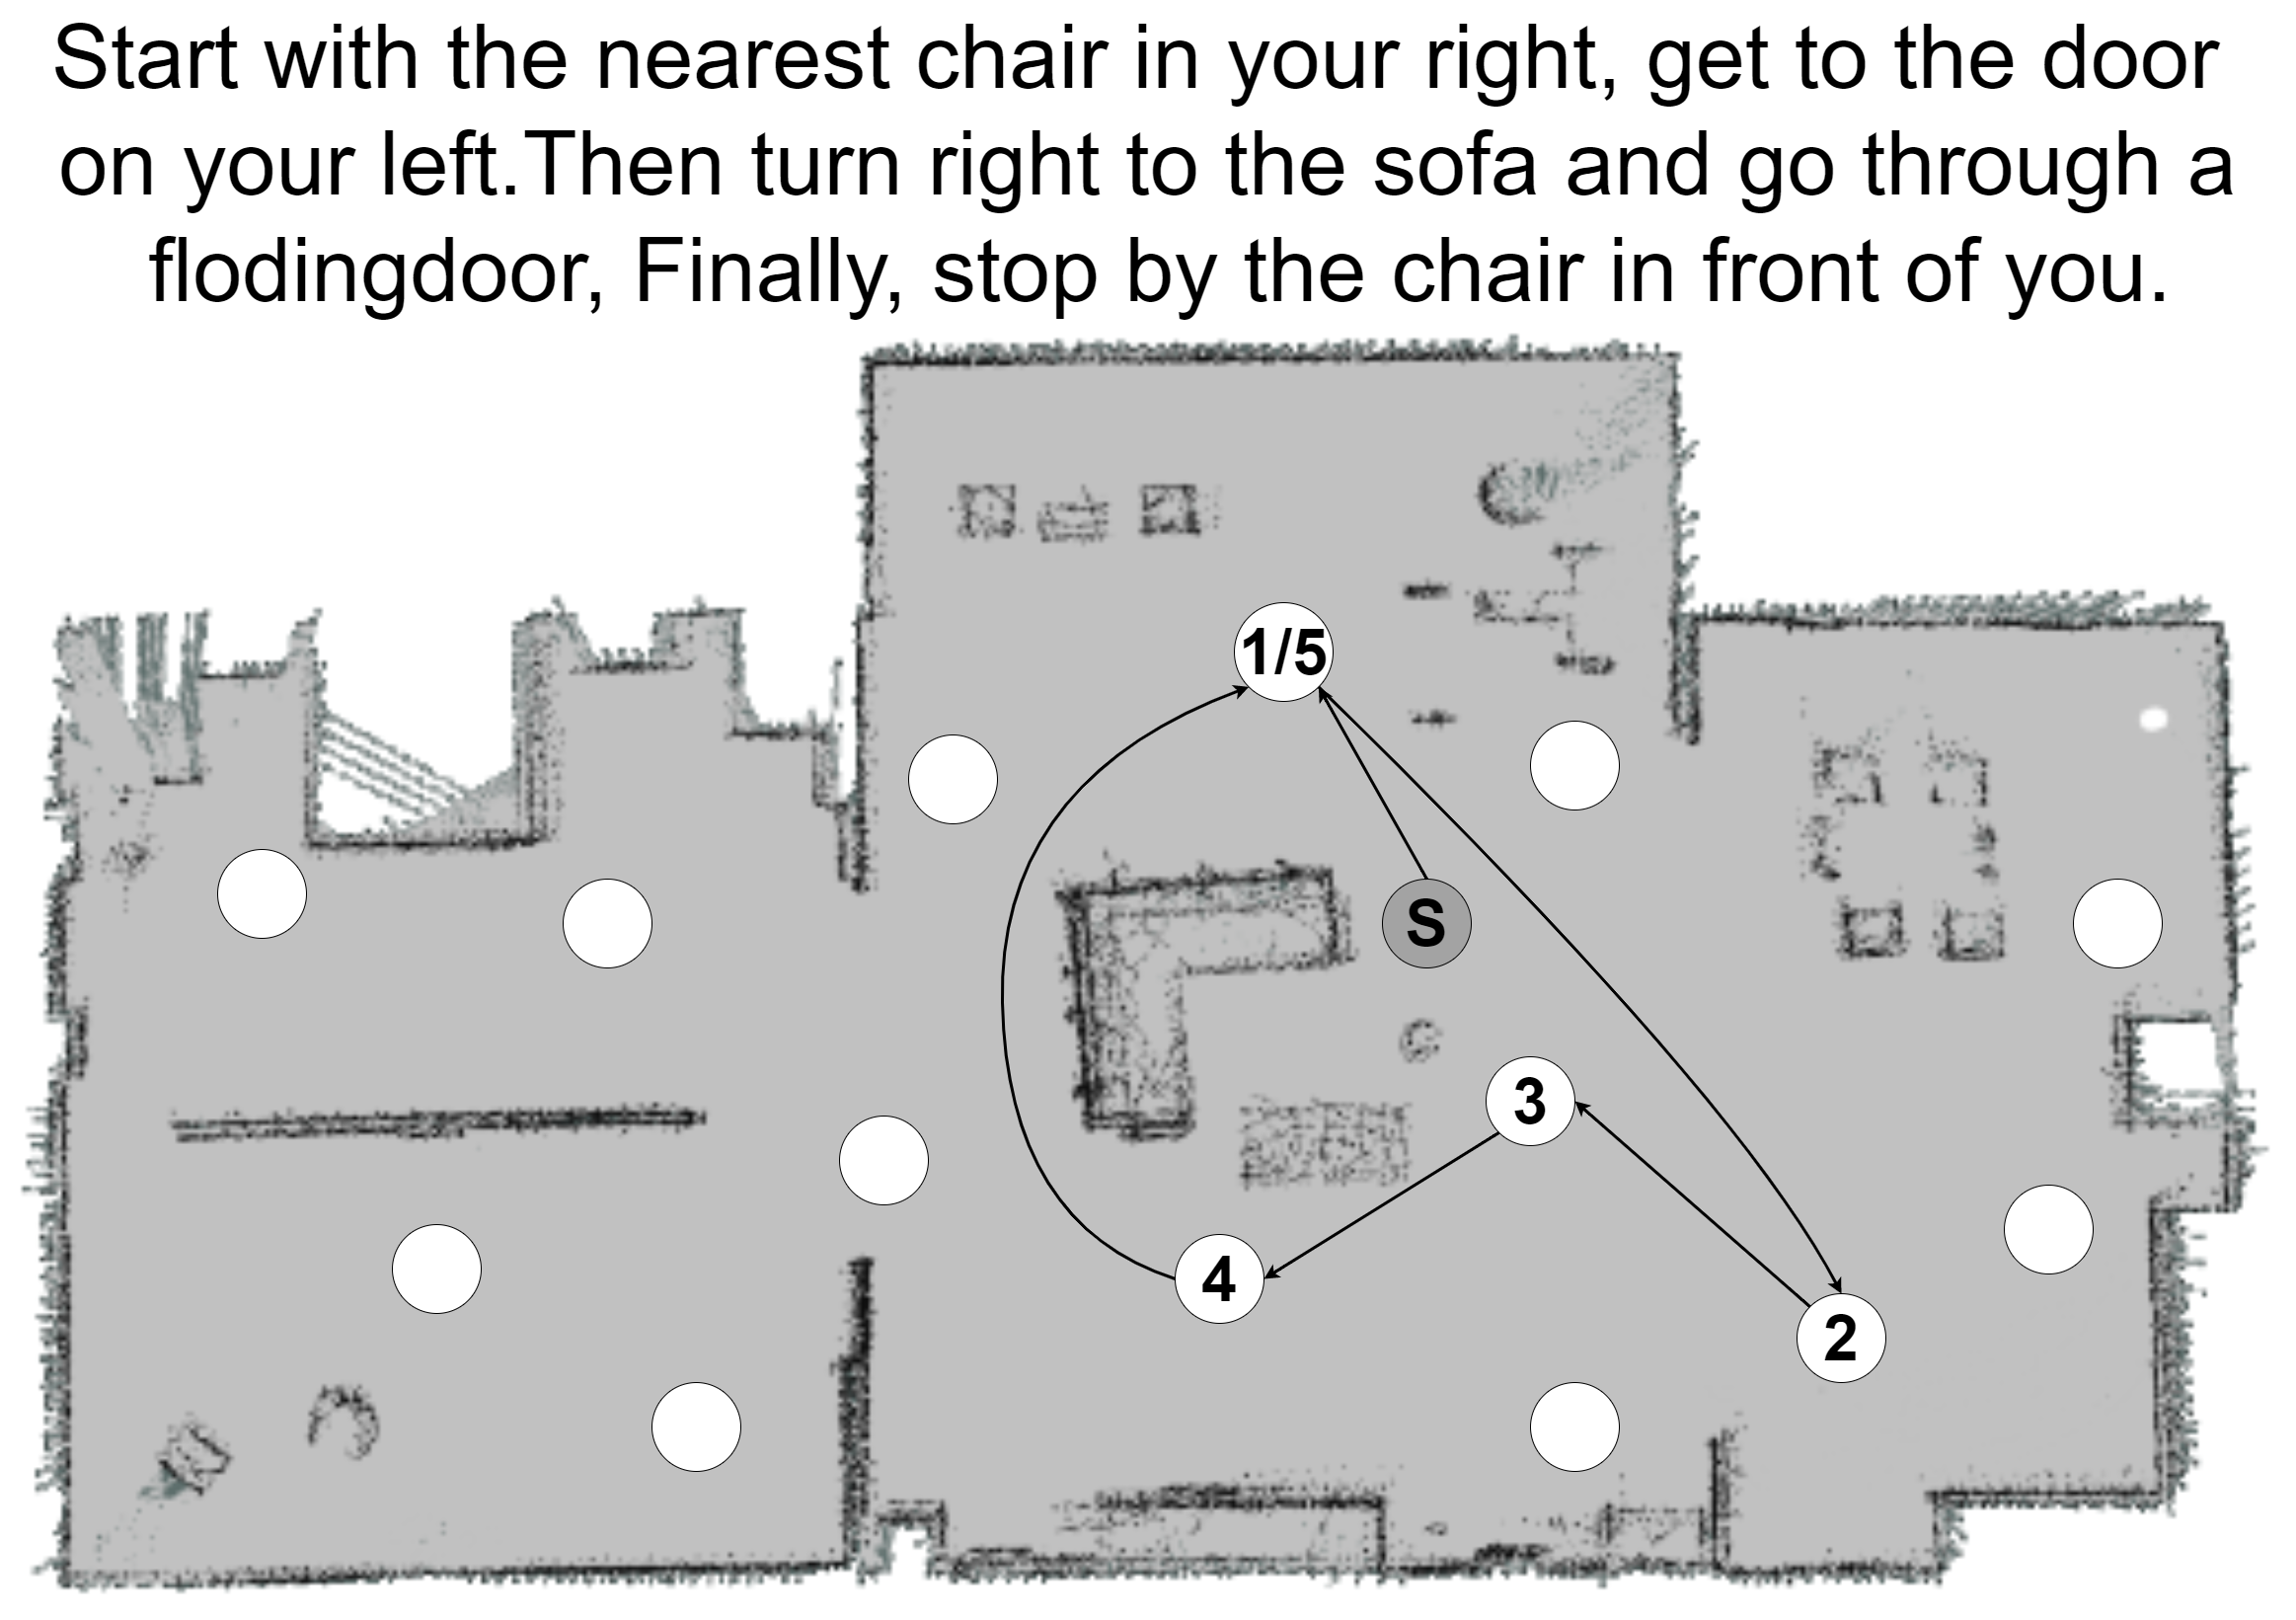
\includegraphics[width=0.5\textwidth]{Fig/消融a.png}}\\
    \subfloat[多模态融合+导航点规划导航路径]{
            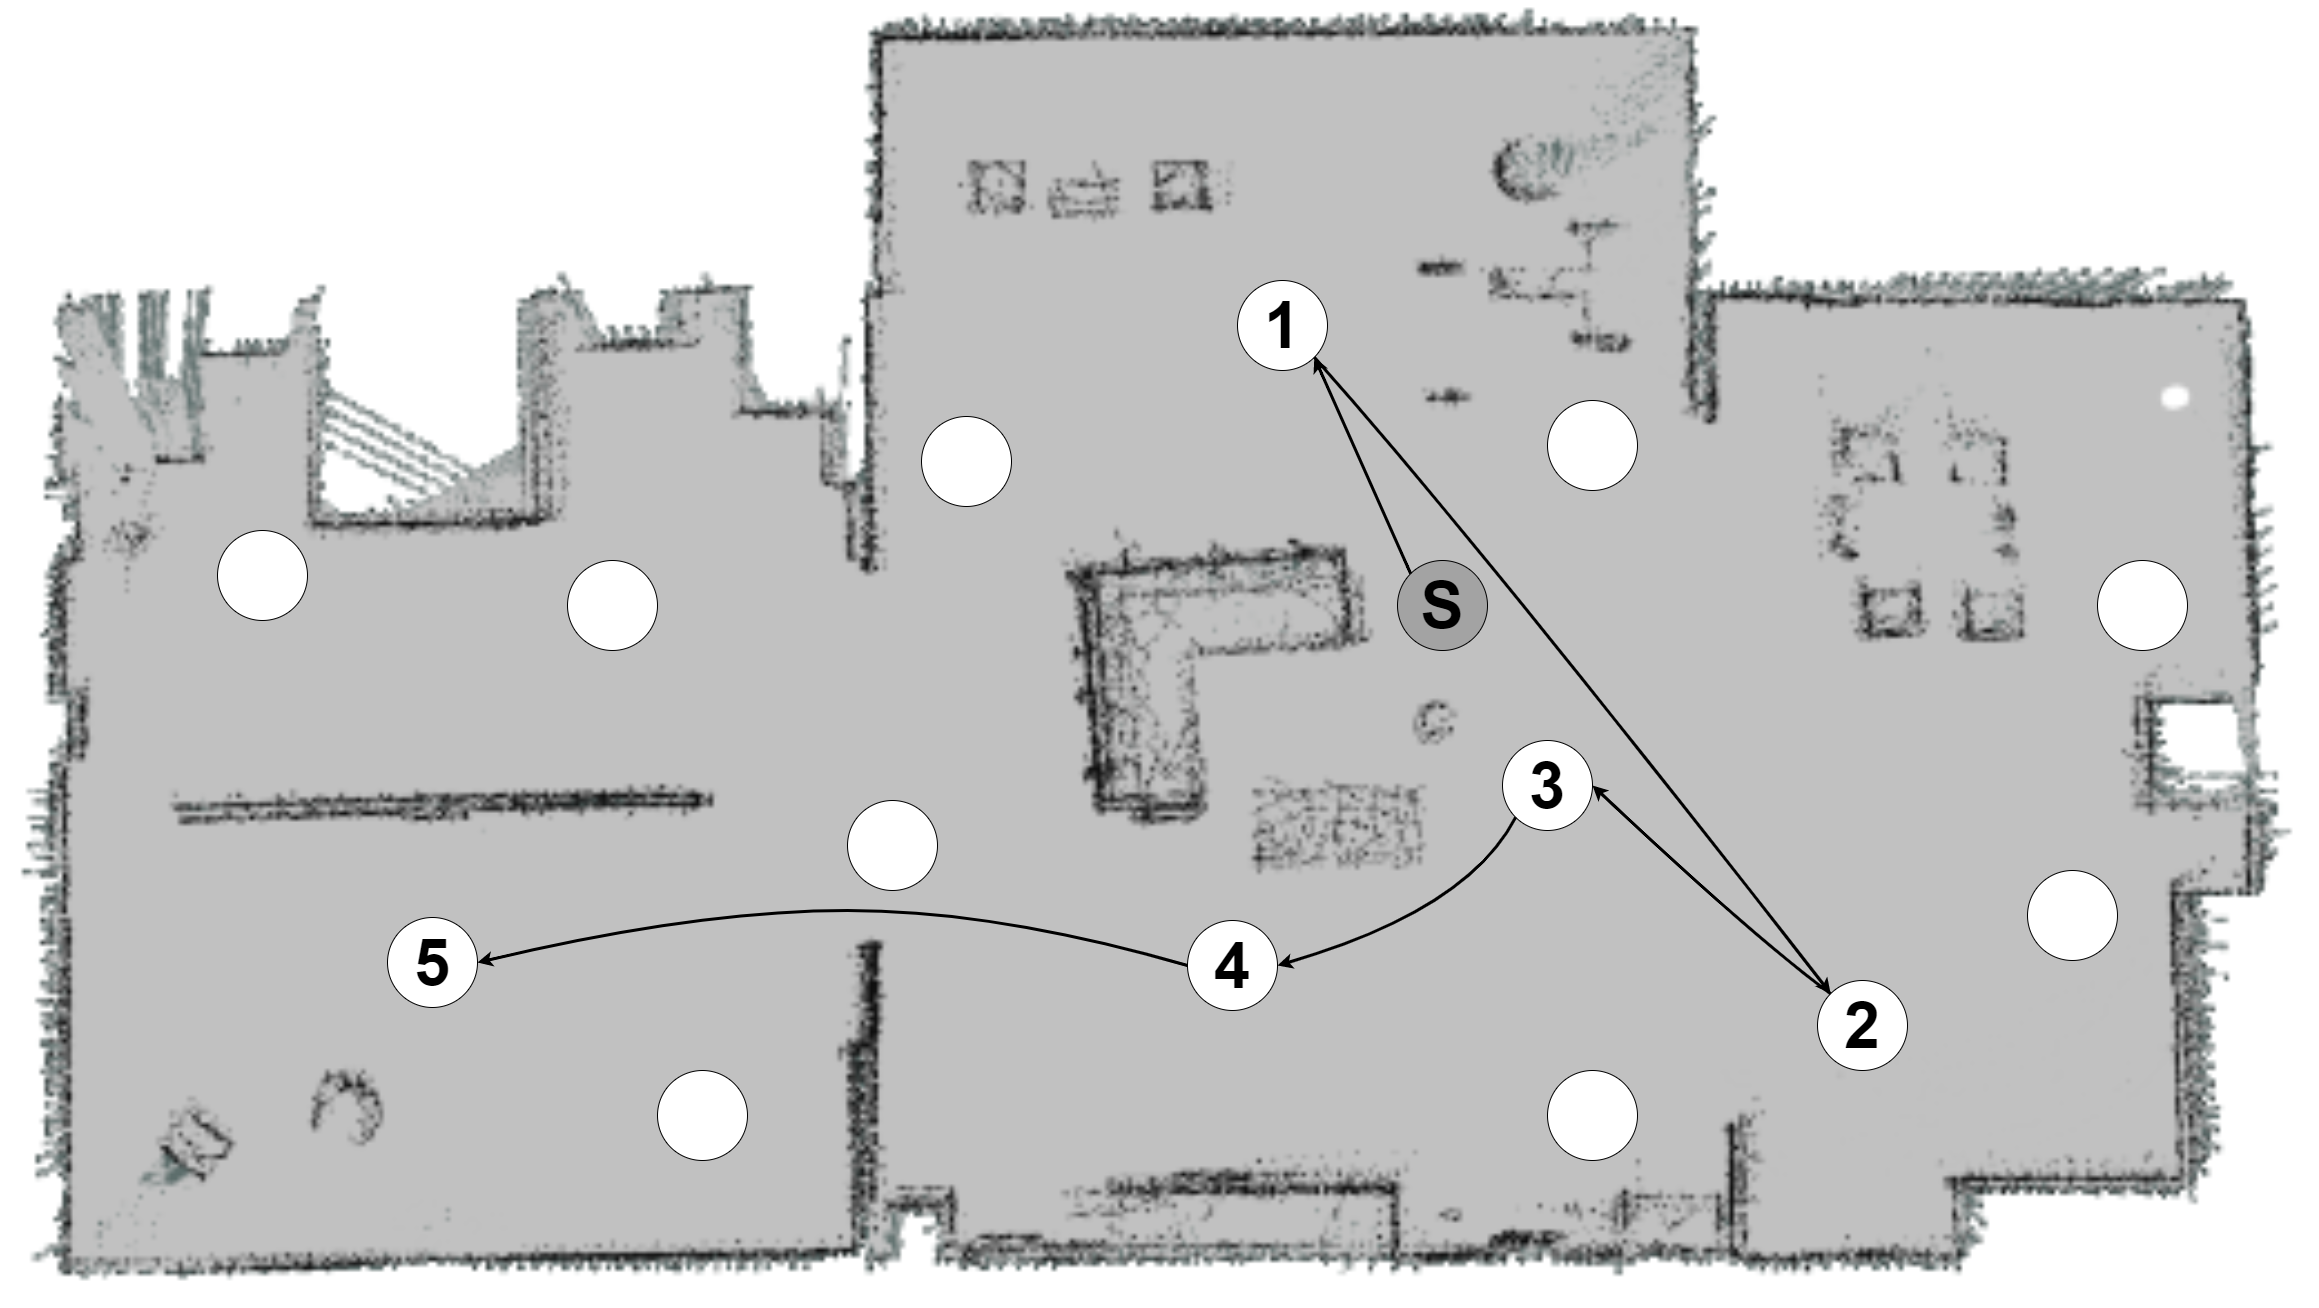
\includegraphics[width=0.5\textwidth]{Fig/消融b.png}}\\
    \subfloat[多模态融合+导航点规划+方位优化导航路径]{
            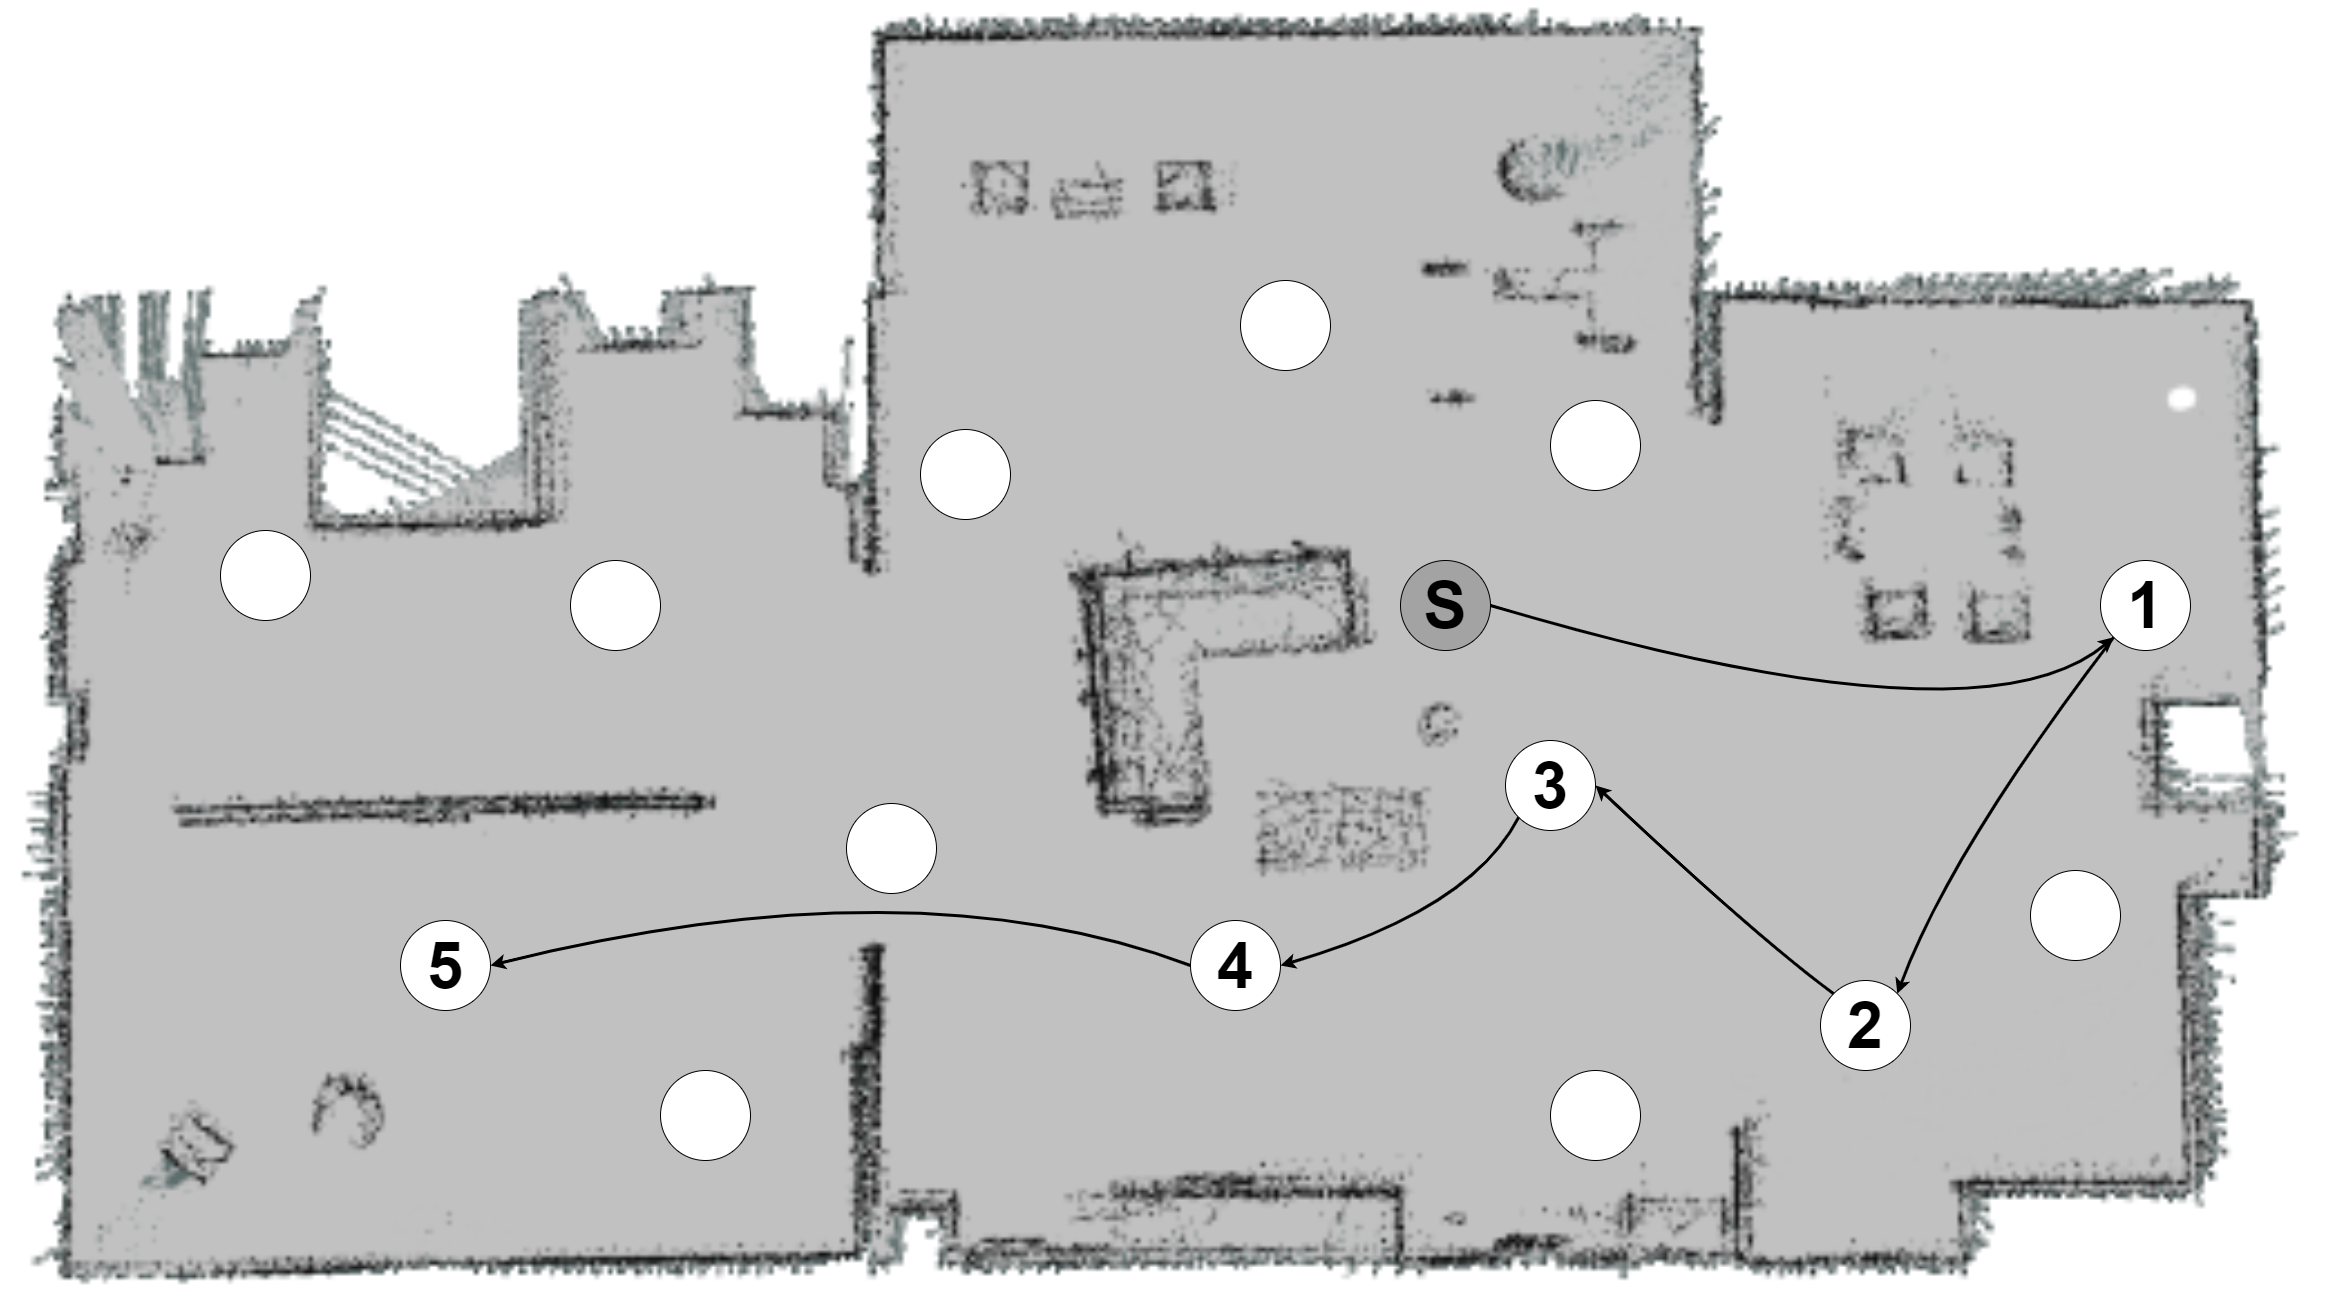
\includegraphics[width=0.5\textwidth]{Fig/消融c.png}}\\
    \subfloat[LVL-Nav方法导航路径]{
                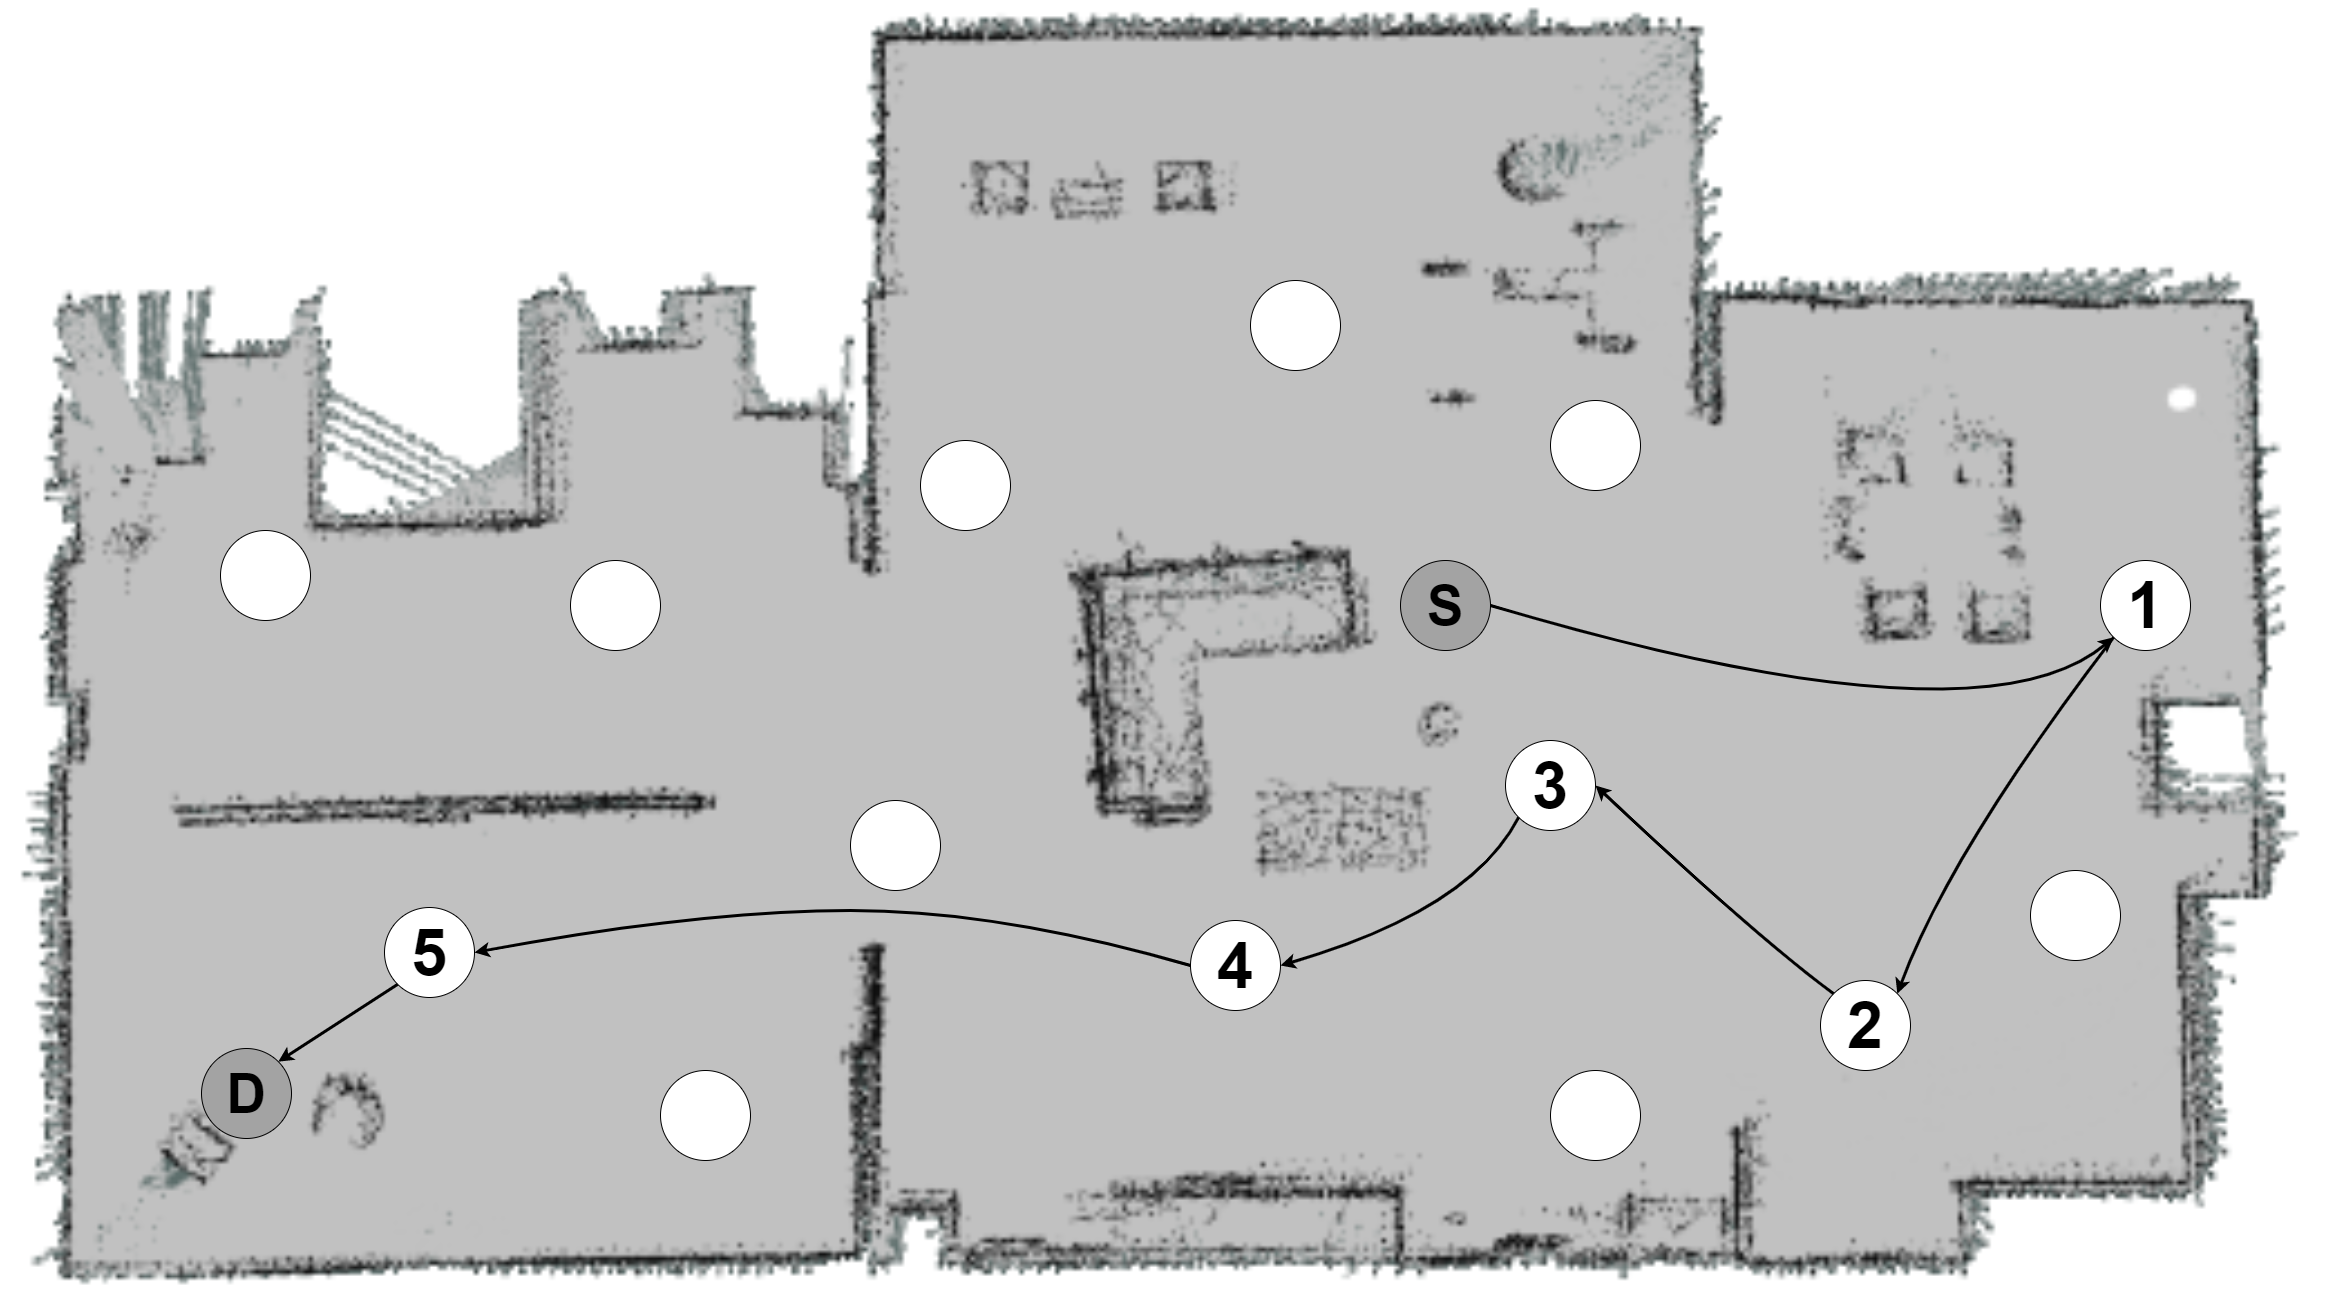
\includegraphics[width=0.5\textwidth]{Fig/消融d.png}}
    \caption{消融实验结果}
    \label{Ablationfig}
\end{figure}
图中$a)$表示仅使用多模态融合网络根据五目标指令所执行的路径和导航到各子目标所捕获的图像,机器人无法利用环境中的距离和方位信息选取导航点、无法区分不同位置的相同目标,错误地选取了1、5两个相同导航点,且无法导航至目标半米内。
$b)$为仅使用多模态融合和导航点规划算法根据相同的五目标指令所执行的导航,机器人无法利用指令中的方位信息,错误地选择左前方最近的椅子作为第一个导航点。
$c)$为仅使用多模态融合、导航点规划和方位优化算法根据相同指令所执行的导航,移动机器人能够正确地通过多模态融合网络进行匹配,再利用导航点规划和方位优化进行筛选,得到了正确的导航点序列,但受限于导航点位姿的初始化,无法完成导航至目标半米内的任务。
$d)$为添加了局部路径规划方法所执行的正确导航,全局路径规划得到了正确的导航点序列,局部路径规划完成导航至目标半米内的任务。


\begin{table}[]
    \caption{\label{Ablationtable}消融实验结果}
    \centering
        \begin{tabular}{cc|c|c|c|c}
        \hline
        \multicolumn{2}{c|}{Method}                     & +多模态融合 & +导航点规划 & +方位优化 & +局部路径规划 \\ \hline
        \multicolumn{1}{c|}{\multirow{2}{*}{I=1}} & SR  & 66.2   & 78.3   & 83.4  & \textbf{88.4}    \\
        \multicolumn{1}{c|}{}                     & SPL & 65.3   & 54.0   & 62.7  & \textbf{66.7}    \\ \hline
        \multicolumn{1}{c|}{\multirow{3}{*}{I=5}} & SR  & 49.6   & 60.9   & 68.1  & \textbf{74.7}    \\
        \multicolumn{1}{c|}{}                     & PMD & 51.9   & 61.7   & 69.4  & \textbf{77.4}    \\
        \multicolumn{1}{c|}{}                     & SPL & 59.3   & 46.6   & 57.2  & \textbf{62.1}    \\ \hline
        \end{tabular}
    \end{table}

对比仿真消融实验结果表明,本文所提出的多模态融合网络、导航点规划、方位优化和局部路径规划算法均能十分有效地帮助移动机器人理解指令目标、利用环境信息,使移动机器人能够根据指令高效且正确地执行导航。









\section{真实环境实验设计与评估}
\subsection{实验设备}%多线激光、开发板参数、移动机器人整体
为进一步验证所提出算法在实际应用中的可行性,选用搭载了镭神C16激光雷达和杰锐微通HF899单目相机的灵遨移动机器人进行真实环境实验,其中激光雷达和用于进行导航实验的移动机器人如图\ref{C16laser}、\ref{mycar}所示。

\begin{figure}[h]
    \centering
    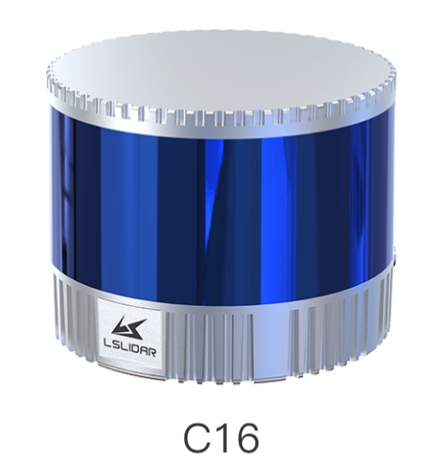
\includegraphics[scale=0.3]{Fig/C16laser.png}
    \caption{\label{C16laser}镭神C16激光雷达}
\end{figure}

\begin{figure}[htbp]
    \centering
    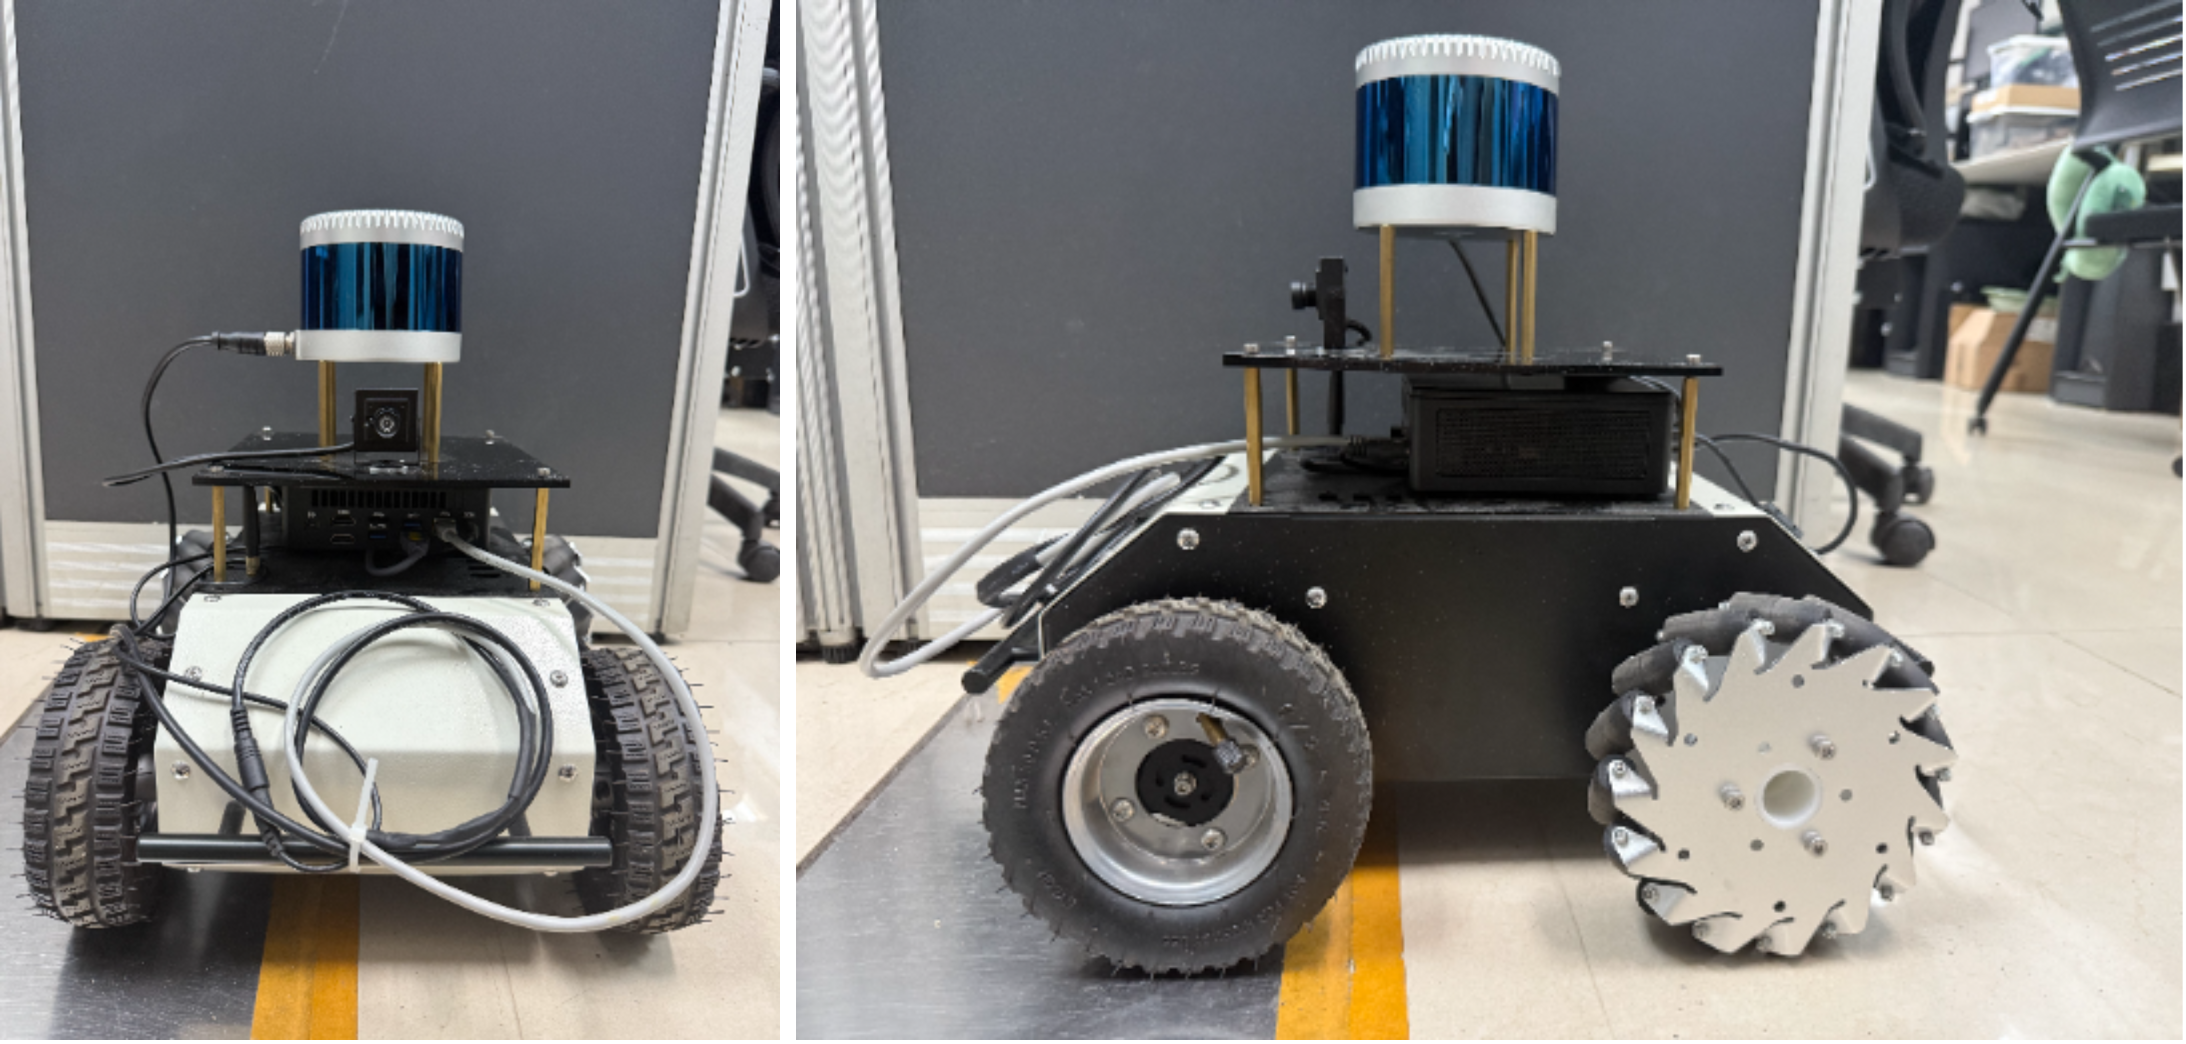
\includegraphics[scale=0.17]{Fig/robot.png}
    \caption{\label{mycar}灵遨移动机器人}
\end{figure}

如表\ref{hardcore}所示,我们将全局路径规划、ROS导航控制系统部署到UP Xtreme i11嵌入式开发板上;将局部路径规划中的特征提取、融合网络模型部署在Jetson TX嵌入式开发板上;灵遨机器人搭载码盘系统,通过IMU等装置实验机器人的移动;镭神C16激光雷达负责全局路径规划中的建图、导肮及局部路径规划中的图像点云融合;杰锐微通HF899单目相机负责局部路径规划中提供第一视觉视觉观察用于特征提取、融合和图像点云融合;其中UP Xtreme i11和Jetson TX嵌入式开发板如图\ref{boardfig}所示,设备的参数如表\ref{Embeddedboard}所示。
\begin{table}
    \caption{\label{hardcore}硬件系统设计}
    \centering
    \small
    \begin{tabular}{cc}
        \hline
        设备 & 功能 \tabularnewline 
        \hline 
        UP Xtreme i11 & 部署全局路径规划、驱动机器人 \tabularnewline
        Jetson TX & 部署导航模型进行探索推理 \tabularnewline
        灵遨机器人 & 移动机器人 \tabularnewline
        镭神C16激光雷达 & 建图、导航及图像点云融合 \tabularnewline
        杰锐微通HF899单目相机 & 获取视觉观察 \tabularnewline
        \hline 
    \end{tabular}
\end{table}


\begin{figure}[h]
    \centering
    %\includegraphics[width=3in]{fig5}
    \subfloat[UP Xtreme i11]{
            \includegraphics[scale=0.071]{Fig/up.jpg}}
    \subfloat[Jetson TX]{
            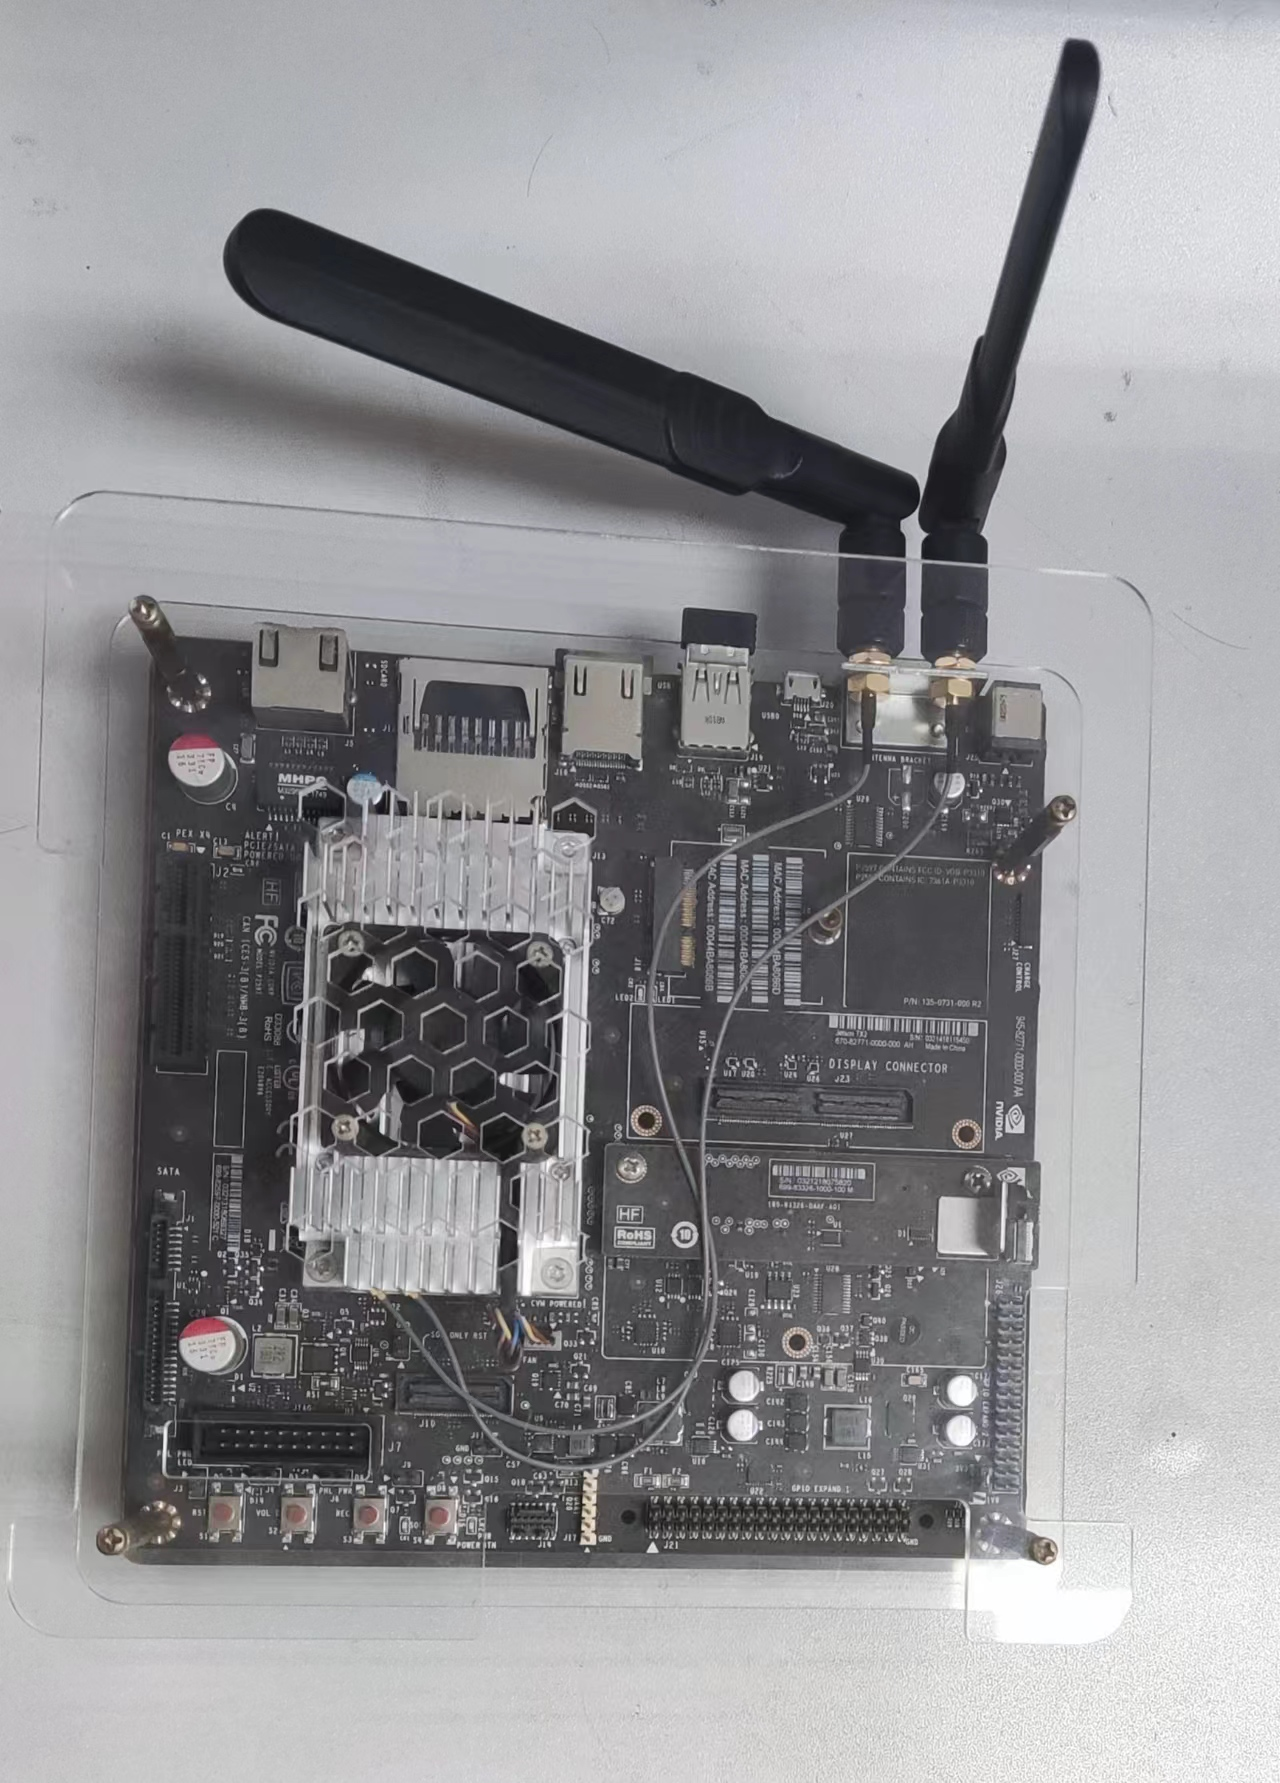
\includegraphics[width=0.34\textwidth]{Fig/Jetsonfig.png}}
    \caption{嵌入式开发板}
    \label{boardfig}
\end{figure}


\begin{table}[]
    \caption{\label{Embeddedboard}硬件设备参数}
    \centering
    \begin{tabular}{c|c|c}
    \hline
    软硬件  & UP Xtreme i11                               & Jetson TX2                                                                                                               \\ \hline
    GPU  & Intel(R)Iris(R) Xe Graphics                 & 256-core NVIDIA Pascal architecture GPU                                                                                  \\
    CPU  & 11th Gen intel r core(tm) i7-1165G7 & \begin{tabular}[c]{@{}c@{}}Dual-core NVIDIA Denver 2 64-bit CPU\\ Quad-core Arm Cortex-A57 MPCore processor\end{tabular} \\
    AI性能 & 1.0TFLOPS                                   & 1.33TFLOPS                                                                                                               \\
    内存   & 2GB                                         & 8GB                                                                                                                      \\
    存储   & 24GB                                        & 32GB                                                                                                                     \\
    功率   & 65w                                         & 7.5w-15w                                                                                                                 \\ \hline
    \end{tabular}
    \end{table}



\subsection{实验环境}
本文的真实实验场景搭建在学院楼内的实验室,总面积约有45平方米。实验场景包含成排的桌子、一个饮水机、一个打印机、两个书架、几张椅子,布局设计成室内办公桌的样式,真实实验环境及其栅格地图如图\ref{myrealenv}所示。我们从22个室内常见物体中随机选择多个连续的指令目标在真实环境中进行实验,包括冰箱、打印机这种不存在复数的目标,也包括椅子、笔记本电脑等这种存在复数的目标。
\begin{figure}[h]
    \centering
    %\includegraphics[width=3in]{fig5}
    \subfloat[真实实验环境]{
            \includegraphics[width=0.70\textwidth]{Fig/realenv.jpg}}\\
    \subfloat[真实实验环境栅格地图]{
            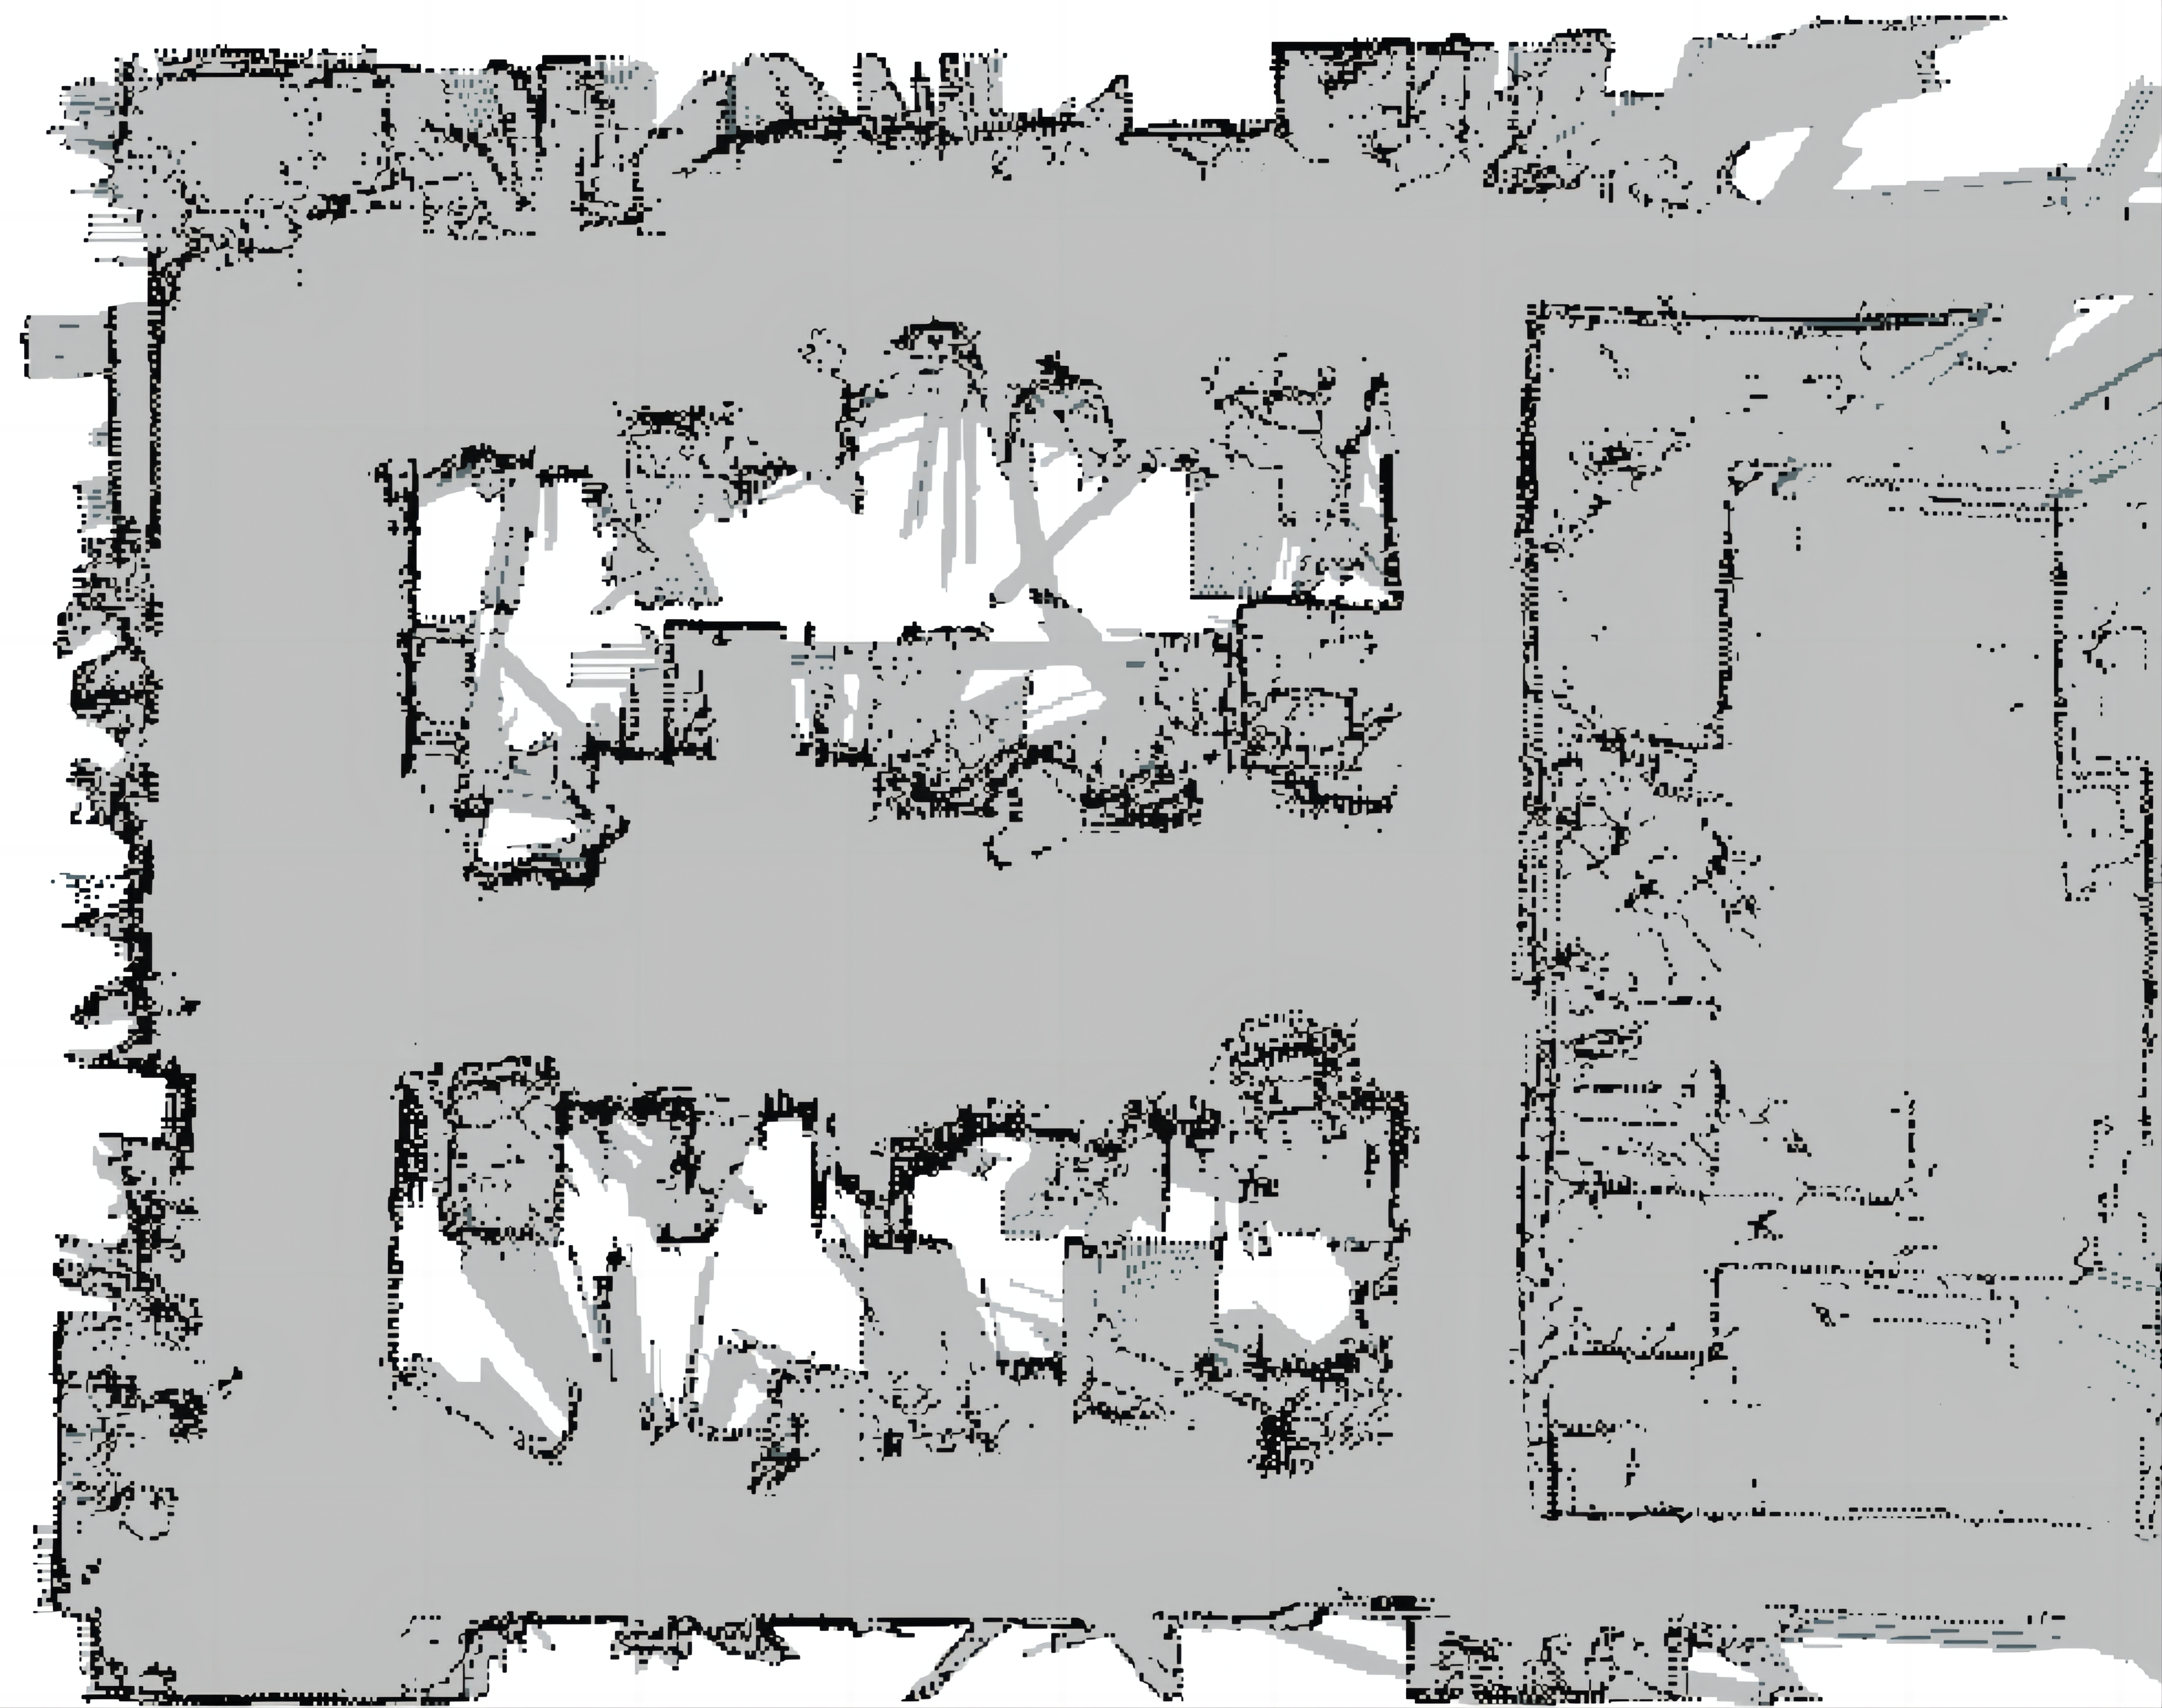
\includegraphics[width=0.70\textwidth]{Fig/realenvmap.jpg}}
    \caption{真实环境}
    \label{myrealenv}
\end{figure}
真实环境中的实验直接使用仿真环境中由全局路径规划和局部路径规划共同构成的LVL-Nav方法进行测试,不在现实测试环境中采集数据来重训练模型,同时也不改变各算法参数,以此来验证所提出的方法在真实环境下的迁移效果,并找出方法的优势和局限。

真实实验的运行环境为内存16GB的64位Ubuntu18.04操作系统,平台为ROS Melodic。通过局域网完成网络连接配置后,使用笔记本电脑执行远程操作,控制机器人完成建图、记录导航点与图像并根据指令执行导航。
在实验的设计上,本文采用随机抽取并随机排序的方法在上述的目标物体中进行选择,在实验环境中也随机布局这些被选中的物体。当移动机器人的局部路径规划在执行完成图像点云融合算法并输出"导航结束"时作为移动机器人完成一次导航的信号,若在导航的过程中正确地根据指令经过所要求的所有目标,并在最后的目标半米内停止则表示本次真实环境下的导航成功,除此之外,在整个导航的过程中若发生过碰撞时间都判定导航失败。



\subsection{导航实验}












实验结果表明,在真实环境下本文提出的导航方法以可靠且高效地根据任意形式的自然语言指令和环境拓扑信息,在光照条件变化大的复杂室内环境中融合感知和认知信息正确规划出全局路径,具备区分导航指令中的细微方向、目标差别的能力,同时局部路径规划允许移动机器人不依赖于环境中导航点位置的设置,正确的导航到目标半米内。

另一方面,我们在测试的过程中也发发现了方法中的不足之处。由于真实环境和仿真环境的差异问题导致了局部路径规划中的特征提取、融合模型性能的下降,当目标未能出现在移动机器人的视觉观察之中时,局部探索方法在存在遮挡物体的环境中存在失败的可能从而导致导航的失败;并且由于真实的室内环境摆放大量的障碍物,这导致移动机器人无法十分有效地在狭窄的环境中进行可靠地导航,在与椅角或桌角发生碰撞后无法继续导航从而导致导航的失败。


\section{本章小结}

本章主要介绍了本文所提出的语言视觉激光多模态融合的机器人导航方法在仿真、真实环境进行目标物体导航的实验,我们通过和近三年表现良好方法的对比试验验证了本文所提出方法的有效性,即通过引入深度信息优化多模态融合网络,提高模型在光线条件变化大的室内的鲁棒性;提出了一种方位优化法筛选不符合方位条件的冗余导航点;通过导航点规划算法进一步提高全局路径规划所生成导航点的正确率;设计了一种特征提取、融合网络能够有效地在局部未知环境中进行探索,设计并实现了一种单目相机和多线激光传感器融合的局部导航方法,以完成导航至目标半米内的闭环任;并进一步通过消融实验分析了所提出方法中各个模块的作用。

实验结果表明,我们所提出的方法在仿真、真实环境中的导航表现基本达到了预期,但受限于真实、仿真环境之间的差异以及真实狭窄环境对局部探索导航和基于目标点导航两方面的影响,移动机器人在真实环境中也存在导航失败的问题亟待解决。 % 新增公式字体设置,需要引入字体包unicode-math然后通过setmainfont设置不同字体(unicode-math包默认Latin Modern Math字体,而latex默认Computer Modern Math字体), Computer Modern Math也是模板一直以来使用的字体。这里提供给需要更多字体的同学探索。模版的修改在scutthesis.cls文件82-85行。若希望探索各种常用数学符号的区别,直接编译math_font文件夹的各种测试文件。注意新的字体包unicode-math包下,加粗,花体等命令都有一定的改变,要适当替换一下。可以在测试文件做好测试再使用。
	% 自行根据需要添加章节。注意要包含正确路径

	\backmatter %章节不编号但页码继续
	%%%%%%%%%%%%%%%%%%%%%%%%%%%%%%%%%%%%%%%%%%%%%%%%%%%%%%%%%%%%%%    微调,使得后续章节的页眉不带章号——by MCH
	\renewcommand{\chaptermark}[1]{\markboth{#1}{}}
	%%%%%%%%%%%%%%%%%%%%%%%%%%%%%%%%%%%%%%%%%%%%%%%%%%%%%%%%%%%%%%
	\chapter{结\texorpdfstring{\quad}{}论}

本文主要研究语言视觉激光多模态融合的机器人导航方法的研究及实现,研究方向是多模态融合的目标物体导航方法,并设计一个导航系统,在移动机器人上部署全局和局部路径规划算法,并在仿真环境和真实环境中进行目标物体导航实验。
	
本文的目标物体导航是在环境中根据多模态的数据到达预期的目标物体。现有的工作通常通过建图来标记环境中存在的目标位置,或是通过训练深度强化学习模型作为代理实时预测动作,以到达指定目标。但上述的方法无法通过视觉信息进行自主探索,忽略了激光雷达所获取的感知信息对于导航的约束和指导,从而导致系统导航成功率低、导航效率低和无法导航到目标半米内的问题。针对以上问题,提出一种多模态融合的目标物体导航方法,具体来说,该方法将导航任务拆分成全局路径规划和局部路径规划两个部分。在全局路径规划中,标记地图中的导航点,保留其位姿、图像、点云图和各点之间的拓扑信息,通过多模态融合网络得到各导航点与目标的匹配权值,结合dijkstra算法和方位优化算法规划出全局路径导航点序列。然后,在局部路径规划中,将多线激光与单目相机进行联合标定,结合目标检测、点云聚类和坐标变换方法得到目标具体位姿,发布导航任务以完成局部路径的规划,实现导航到目标半米内的闭环任务。Gazebo数据集上的实验表明,该方法在测试环境中优于最先进的方法,实验结果证明了该方法的有效性和效率。多模态融合的导航系统具有环境感知、目标认知、路径规划和自主导航四个方面的功能,可以完成真实环境下目标物体导航任务。

总的来说,本文的主要贡献如下:
\begin{enumerate}[topsep = 0 pt, itemsep= 0 pt, parsep=0pt, partopsep=0pt, leftmargin=44pt, itemindent=0pt, labelsep=6pt, label=(\arabic*)]
    \item 	本文提出了一种全局路径规划导航方法。与前人的工作相比,针对静态目标导航任务所提出的全局路径规划导航方法基于单目相机、激光雷达等多种传感器和基于多模态特征融合神经网络,增强系统对当前环境和导航过程中的认知和感知能力,再通过方位优化算法筛除噪声导航点,提高导航点选择的正确率的同时提高后续规划的计算响应速度,最后通过导航点规划算法加权融合多种策略进一步提高导航的准确率和导航效率。实验结果表明该方法具有一定的有效性和优越性。
    \item	本文提出了一种未知环境的目标物体探索方法。与前人的工作相比,针对动态目标导航任务所提出的局部目标物体探索方法基于多特征提取和融合的方法,在同一嵌入空间内利用注意力机制融合视觉特征和文本特征,有效的构建了视觉表示和目标物体所在导航方向的关联,使系统能够通过探索找到在变化的环境中的目标物体。
    \item	本文设计了一套单目相机和多线激光融合的图像点云融合方法,联合视觉观察的认知信息和多线点云的感知信息让移动机器人能够有效地在仿真环境和真实环境中依据自然语言指令完成目标导航任务,在移动机器人平台对所提出方法进行了测试加以验证。
\end{enumerate}



本文专注于研究一种适用于室内服务机器人的目标物体导航方法,并致力于构建一个可以部署在真实移动机器人上的语言视觉激光多模态融合的导航系统,使移动机器人既能根据自然语言指令进行全局路径规划,完成导航至目标半米内的任务。多模态融合导航系统具有环境认知与感知、路径规划和自主导航探索这三个主要方面的功能,可以完成室内真实环境下的多目标物体导航任务,该方法在多目标物体连续导航的仿真测试环境中优于最先进的方法,实验结果证明了该方法的有效性和效率。对于未来的展望,本文有以下三个方向可以进行考虑:
\begin{enumerate}[topsep = 0 pt, itemsep= 0 pt, parsep=0pt, partopsep=0pt, leftmargin=44pt, itemindent=0pt, labelsep=6pt, label=(\arabic*)]
    \item 	在真实环境的导航实验之中,我们采用激光雷达结合低功耗计算平台的导航架构在常规场景下表现稳定,但在复杂狭窄环境等受限空间内导航系统对误差源的容忍性下降,容易出现轨迹规划失效、运动控制失稳等问题。可以根据地图中障碍物与全局路径的几何关系标记狭窄环境并生成合适通行位姿对,在机器人出入被标记的狭窄环境时自动切换相应导航策略。通过这种全局成本地图膨胀化以规划更安全的全局路径的方法,机器人根据合适通行位姿分段规划全局路径以自适应环境
    \item	在真实环境的导航实验之中,由于真实环境和仿真环境的差异问题导致了局部路径规划中的特征提取、融合模型性能的下降,当移动机器人在存在行人、移动的椅子等动态的环境中进行导航时,局部探索方法会因遮挡物体的存在而发生碰撞从而导致导航的失败。可以通过在局部路径规划的特征提取模块加入视觉观察的深度图,帮助模型更精准地定位物体的位置信息、理解环境的拓扑结构和空间关系,进一步提高模型对于空间中的物体位置的感知,从而更高效、可靠地执行局部探索任务。
    \item	目标物体导航的环境中存在众多不同尺寸的物体,而多尺度特征可以增强模型的鲁棒性使其更具有抗干扰性,因此可以考虑添加多尺度特征可以更好地适应不同尺度下的物体。不同尺度的特征可以在不同的情况下提供更好的表征,让模型能够更好地应对光照变化、遮挡、旋转等因素的影响。另一方面,添加多尺度特征会增加计算复杂度,可以通过金字塔结构或多尺度卷积等方法共享计算从而提高效率。这种方法能够提供更丰富的语义信息、适应不同尺度的物体、增强模型的鲁棒性,并且能够更好地结合局部和全局信息,从而提高图像处理任务的性能和效率。 
    
\end{enumerate}


 %结论
	 %%%%%%%%%%%%%%%%%%%%%%%%%%%%%%%%%%%%%%%%%%%%%% bibtex参考文献设置  (原版)
%%	\bibliographystyle{scutthesis}
%%	\bibliography{F:/MyLibrary}
	%%%%%%%%%%%%%%%%%%%%%%%%%%%%%%%%%%%%%%%%%%%%%%
	%%%%%%%%%%%%%%%%%%%%%%%%%%%%%%%%%%%%%%%%%%%%%% biber参考文献设置	——by MCH
	%\renewcommand*{\bibfont}{\refbodyfont}			% 设置文献著录字号比正文小一号(五号),需要小四号请注释该行. % 不推荐使用small,而是使用cls文件中精确定义了的字号。
	\phantomsection % “目录”中的链接能正确跳转,需要添加 \phantomsection 否则点击参考文献会跳转到结论
	\addcontentsline{toc}{chapter}{参考文献}	%目录中添加参考文献
	\printbibliography	% 参考文献著录
 	%%%%%%%%%%%%%%%%%%%%%%%%%%%%%%%%%%%%%%%%%%%%%%
 	% 只有一个附录
% 	%%%%%%%%%%%%%%%%%%%此部分为附录环境代码,是比较笨的方法来适应论文撰写规范%%%%%%%%%%%%%%%%%%%%%%%%%%%%%%%%%%%%%%
%对只有一个附录,标题不编号比较美观。
%%%%%%%%%%%%%%%%%%%%%%%%%%%%%%%%%%%%%%%%%%%%%%%%%%%%%%%%%%%%%%%%%%%%%%%%%%%%%%%%%%%%%%%%%%%%%%%%%%%%%%%%%%%%
\setcounter{chapter}{1} %从1开始编号
\setcounter{section}{0}
\setcounter{equation}{0}
\setcounter{table}{0}   
\setcounter{figure}{0}
\chapter{附\texorpdfstring{\quad}{}录} %附录
%%%%%%%%%%%%%%%%%%%%%%%%%%%%%%%%%%%%%%%%%%%%%%%%%%%%%%%%%%%%%%%%%%%%%%%%%%%%%%%%%%%%%%%%%%%%%%%%%%%%%%%%
%%%%%%%%%%%%以下为用户代码,用于撰写您的论文%%%%%%%%%%%%%%%%%%%%%%%%%%%%%%%%%%%%%%%%%%%%%%%%%%%%%%%%%%%%%%


在论文撰写规范中,下面两段话让人费解:

\begin{enumerate}
	\item 	对需要收录于学位论文中但又不适合书写于正文中的附加数据、方案、资料、详细公式推导、计算机程序、统计表、注释等有特色的内容,可做为附录排写,序号采用“附录1”、“附录2”等。	
	\item	公式序号按章编排,如第一章第一个公式序号为“(1-1)”,附录2中的第一个公式为“(2-1)”等。
\end{enumerate}

论文撰写规范要求的附录和通常书籍上使用附录A、附录B等编号的不一样,容易和正文混淆。特殊的要求和代码的耦合,使我不得不使用比较笨的方法来设计附录部分的模板。

\section{测试测试测试}
\subsection{测试测试测试}
%
测试测试测试测试测试测试测试测试测试测试测试测试测试测试测试测试测试测试测试测试测试测试测试测试测试测试测试测试测试测试测试测试测试测试测试测试测试测试测试测试测试测试测试测试测试测试测试测试测试测试测试测试测试测试测试测试测试测试测试测试测试测试测试测试测试测试测试测试测试测试测试测试测试测试测试测试测试测试测试测试测试测试测试测试测试测试测试测试测试测试测试测试测试测试测试测试测试测试测试测试测试测试测试测试测试测试测试测试测试测试测试测试测试测试测试测试测试测试测试测试测试测试测试测试测试测试测试测试测试测试测试测试测试测试测试测试测试测试测试测试测试测试测试测试测试测试测试测试测试测试测试测试测试
\begin{align}
\left\{\begin{array}{l}
\dot{v}_{1}(t)=v_{2}(t) \\
\dot{v}_{2}(t)=R^{2}\left(-\zeta_{1}\left[v_{1}(t)-v_c(t)\right]^{\alpha}-\zeta_{2}\left[\dfrac{v_{2}(t)}{R}\right]^{\beta}\right)
\end{array}\right.	
\end{align}

\begin{align}
\left\{\begin{array}{l}
\dot{v}_{1}(t)=v_{2}(t) \\
\dot{v}_{2}(t)=R^{2}\left(-\zeta_{1}\left[v_{1}(t)-v_c(t)\right]^{\alpha}-\zeta_{2}\left[\dfrac{v_{2}(t)}{R}\right]^{\beta}\right)
\end{array}\right.	
\end{align}
\begin{figure}[htbp]
	\centering	
	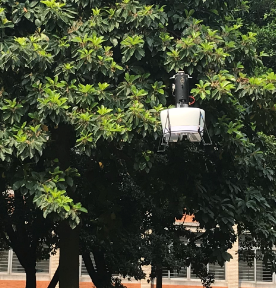
\includegraphics[scale=1]{Fig/DFUAV_f31.png}
	\caption{\label{fig_case1}测试测试测试}
\end{figure}
\begin{figure}[htbp]
	\centering	
	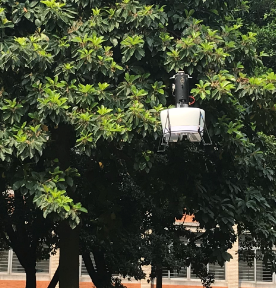
\includegraphics[scale=1]{Fig/DFUAV_f31.png}
	\caption{\label{fig_case2}测试测试测试}
\end{figure}
\begin{table}
	\caption{\label{DF_para1}测试测试测试}
	\centering{}%
	\small 
	\begin{tabular}{cccccc}
		\hline 
		参数符号 & 数值&参数符号 & 数值&参数符号 & 数值\tabularnewline
		\hline 
		$ A_x,A_y,A_z $  & $ 0.04082\,\text{m}^2 $ &$ \rho $        &$1.225\,\text{kg}/\text{m}^3$&$ I_b $           & $ 0.000029 $               \tabularnewline
		$ k_{\varpi} $   & $1.13342 \times 10^{-6}$& $ d_{\varpi} $ & $1.13342 \times 10^{-7}$ 	  &$k_{\delta} $     & $ 0.01495 $ 			      \tabularnewline
		$C_{D,x},C_{D,y}$& $ 0.43213 $             &$ C_{D,z} $     & $ 0.13421 $             	  &	$ q_a $ 	     & $ 1.49 $ 				  \tabularnewline
		$ l_{a} $        & $ -0.1121\,\text{m} $   & $ d_{ds} $     & $ 0.01495 $			  	  &$ d_{af} $        & $ 0.01495 $    			  \tabularnewline
		$ R $            & $ 0.11\,\text{m} $      &$ b $           & $ 2 $       			   	  &$ S $ 			 & $ 0.04082\,\text{m}^2 $    \tabularnewline
		$C_{l_{\alpha}}$ & $ 2.212\,/\text{rad} $  &$C_{l, \max } $ & $ 1.05 $ 				   	  &$ C_{l, \min } $  & $ -1.05 $ 				  \tabularnewline
		$ l_2 $          & $ 0.06647\,\text{m} $   &$ l_1 $         & $ 0.17078\,\text{m} $    	  &	$ m $ 		     & $ 1.53\,\text{kg} $ 		  \tabularnewline
		$ C_{d, o } $    & $ 0.9 $                 &$ C_{d, g } $   & $ 0.9 $					  &$ C_{duct} $      & $ 0.78497 $	 			  \tabularnewline
		$ I_x $          & $ 0.02548 $ 			   &$ I_y $         & $ 0.02550 $                 &$ I_z $			 & $ 0.00562 $ 				  \tabularnewline
		\hline 
	\end{tabular}	
\end{table}

\begin{table}
	\caption{\label{TDF_para2}测试测试测试}
	\centering{}%
	\small 
	%	\resizebox{\textwidth}{!}{
	\begin{tabular}{cccccc}
		\hline 
		参数符号 & 数值&参数符号 & 数值&参数符号 & 数值\tabularnewline
		\hline 
		$ I_x $ & $ 054593 $ &$ I_y $ & $ 0.017045 $& $ I_z$ & $ 0.049226 $ \tabularnewline
		$ l_{1} $ & $ 0.0808\,\text{m} $&$ l_{2} $ & $ 0.175\,\text{m} $ &$ l_3 $ & $ 0.06647\,\text{m} $ \tabularnewline 
		$ l_4 $ & $ 0.2415\,\text{m} $ &$ l_5 $ & $ 0.1085\,\text{m} $& $ m $ & $ 3.7\,\text{kg} $ \tabularnewline
		\hline 
	\end{tabular}	%}
\end{table}

\section{测试测试测试}
\subsection{测试测试测试}
%
测试测试测试测试测试测试测试测试测试测试测试测试测试测试测试测试测试测试测试测试测试测试测试测试测试测试测试测试测试测试测试测试测试测试测试测试测试测试测试测试测试测试测试测试测试测试测试测试测试测试测试测试测试测试测试测试测试测试测试测试测试测试测试测试测试测试测试测试测试测试测试测试测试测试测试测试测试测试测试测试测试测试测试测试测试测试测试测试测试测试测试测试测试测试测试测试测试测试测试测试测试测试



 	% 有多个附录
	%%%%%%%%%%%%%%%%%%%%此部分为附录1环境代码,是比较笨的方法来适应论文撰写规范%%%%%%%%%%%%%%%%%%%%%%%%%%%%%%%%%%%%%%
%新增附录时只需要将\setcounter{chapter}{X}以及\chapter{附\texorpdfstring{\quad}{}录 X}中相应的X更改为
%相应的数字,如果只有一个附录,则选用appendix
%%%%%%%%%%%%%%%%%%%%%%%%%%%%%%%%%%%%%%%%%%%%%%%%%%%%%%%%%%%%%%%%%%%%%%%%%%%%%%%%%%%%%%%%%%%%%%%%%%%%%%%%%%%%
\setcounter{chapter}{1} %从1开始编号
\setcounter{section}{0}
\setcounter{equation}{0}
\setcounter{table}{0}   
\setcounter{figure}{0}
\chapter{附\texorpdfstring{\quad}{}录 1} %附录1
%%%%%%%%%%%%%%%%%%%%%%%%%%%%%%%%%%%%%%%%%%%%%%%%%%%%%%%%%%%%%%%%%%%%%%%%%%%%%%%%%%%%%%%%%%%%%%%%%%%%%%%%
%%%%%%%%%%%%以下为用户代码,用于撰写您的论文%%%%%%%%%%%%%%%%%%%%%%%%%%%%%%%%%%%%%%%%%%%%%%%%%%%%%%%%%%%%%%

在论文撰写规范中,下面两段话让人费解:

\begin{enumerate}
	\item 	对需要收录于学位论文中但又不适合书写于正文中的附加数据、方案、资料、详细公式推导、计算机程序、统计表、注释等有特色的内容,可做为附录排写,序号采用“附录1”、“附录2”等。	
	\item	公式序号按章编排,如第一章第一个公式序号为“(1-1)”,附录2中的第一个公式为“(2-1)”等。
\end{enumerate}

论文撰写规范要求的附录和通常书籍上使用附录A、附录B等编号的不一样,容易和正文混淆。特殊的要求和代码的耦合,使我不得不使用比较笨的方法来设计附录部分的模板。这部分还需要有附录需求的同学来完善,为了目录中美观且不命名冲突,还是不在附录使用图表。


\section{测试一级标题 section}
\subsection{测试二级标题 subsection}
\subsubsection{测试三级标题 subsubsection}
%
测试测试测试测试测试测试测试测试测试测试测试测试测试测试测试测试测试测试测试测试测试测试测试测试测试测试测试测试测试测试测试测试测试测试测试测试测试测试测试测试测试测试测试测试测试测试测试测试测试测试测试测试测试测试测试测试测试测试测试测试测试测试测试测试测试测试测试测试测试测试测试测试测试测试测试测试测试测试测试测试测试测试测试测试测试测试测试测试测试测试测试测试测试测试测试测试测试测试测试测试测试测试测试测试测试测试测试测试测试测试测试测试测试测试测试测试测试测试测试测试测试测试测试测试测试测试测试测试测试测试测试测试测试测试测试测试测试测试测试测试测试测试测试测试测试测试测试测试测试测试测试测试测试
\begin{align}
\left\{\begin{array}{l}
\dot{v}_{1}(t)=v_{2}(t) \\
\dot{v}_{2}(t)=R^{2}\left(-\zeta_{1}\left[v_{1}(t)-v_c(t)\right]^{\alpha}-\zeta_{2}\left[\dfrac{v_{2}(t)}{R}\right]^{\beta}\right)
\end{array}\right.	
\end{align}

\begin{align}
\left\{\begin{array}{l}
\dot{v}_{1}(t)=v_{2}(t) \\
\dot{v}_{2}(t)=R^{2}\left(-\zeta_{1}\left[v_{1}(t)-v_c(t)\right]^{\alpha}-\zeta_{2}\left[\dfrac{v_{2}(t)}{R}\right]^{\beta}\right)
\end{array}\right.	
\end{align}
% \begin{figure}[htbp]
% 	\centering	
% 	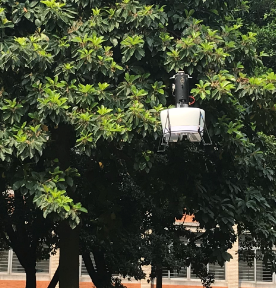
\includegraphics[scale=1]{Fig/DFUAV_f31.png}
% 	\caption{\label{fig_case1}测试测试测试}
% \end{figure}
% \begin{figure}[htbp]
% 	\centering	
% 	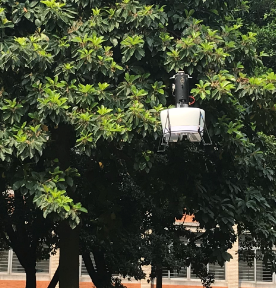
\includegraphics[scale=1]{Fig/DFUAV_f31.png}
% 	\caption{\label{fig_case2}测试测试测试}
% \end{figure}
% \begin{table}
% 	\caption{\label{DF_para1}测试测试测试}
% 	\centering{}%
% 	\small 
% 	\begin{tabular}{cccccc}
% 		\hline 
% 		参数符号 & 数值&参数符号 & 数值&参数符号 & 数值\tabularnewline
% 		\hline 
% 		$ A_x,A_y,A_z $  & $ 0.04082\,\text{m}^2 $ &$ \rho $        &$1.225\,\text{kg}/\text{m}^3$&$ I_b $           & $ 0.000029 $               \tabularnewline
% 		$ k_{\varpi} $   & $1.13342 \times 10^{-6}$& $ d_{\varpi} $ & $1.13342 \times 10^{-7}$ 	  &$k_{\delta} $     & $ 0.01495 $ 			      \tabularnewline
% 		$C_{D,x},C_{D,y}$& $ 0.43213 $             &$ C_{D,z} $     & $ 0.13421 $             	  &	$ q_a $ 	     & $ 1.49 $ 				  \tabularnewline
% 		$ l_{a} $        & $ -0.1121\,\text{m} $   & $ d_{ds} $     & $ 0.01495 $			  	  &$ d_{af} $        & $ 0.01495 $    			  \tabularnewline
% 		$ R $            & $ 0.11\,\text{m} $      &$ b $           & $ 2 $       			   	  &$ S $ 			 & $ 0.04082\,\text{m}^2 $    \tabularnewline
% 		$C_{l_{\alpha}}$ & $ 2.212\,/\text{rad} $  &$C_{l, \max } $ & $ 1.05 $ 				   	  &$ C_{l, \min } $  & $ -1.05 $ 				  \tabularnewline
% 		$ l_2 $          & $ 0.06647\,\text{m} $   &$ l_1 $         & $ 0.17078\,\text{m} $    	  &	$ m $ 		     & $ 1.53\,\text{kg} $ 		  \tabularnewline
% 		$ C_{d, o } $    & $ 0.9 $                 &$ C_{d, g } $   & $ 0.9 $					  &$ C_{duct} $      & $ 0.78497 $	 			  \tabularnewline
% 		$ I_x $          & $ 0.02548 $ 			   &$ I_y $         & $ 0.02550 $                 &$ I_z $			 & $ 0.00562 $ 				  \tabularnewline
% 		\hline 
% 	\end{tabular}	
% \end{table}

% \begin{table}
% 	\caption{\label{TDF_para2}测试测试测试}
% 	\centering{}%
% 	\small 
% 	%	\resizebox{\textwidth}{!}{
% 	\begin{tabular}{cccccc}
% 		\hline 
% 		参数符号 & 数值&参数符号 & 数值&参数符号 & 数值\tabularnewline
% 		\hline 
% 		$ I_x $ & $ 054593 $ &$ I_y $ & $ 0.017045 $& $ I_z$ & $ 0.049226 $ \tabularnewline
% 		$ l_{1} $ & $ 0.0808\,\text{m} $&$ l_{2} $ & $ 0.175\,\text{m} $ &$ l_3 $ & $ 0.06647\,\text{m} $ \tabularnewline 
% 		$ l_4 $ & $ 0.2415\,\text{m} $ &$ l_5 $ & $ 0.1085\,\text{m} $& $ m $ & $ 3.7\,\text{kg} $ \tabularnewline
% 		\hline 
% 	\end{tabular}	%}
% \end{table}

\section{测试测试测试}
\subsection{测试测试测试}
%
测试测试测试测试测试测试测试测试测试测试测试测试测试测试测试测试测试测试测试测试测试测试测试测试测试测试测试测试测试测试测试测试测试测试测试测试测试测试测试测试测试测试测试测试测试测试测试测试测试测试测试测试测试测试测试测试测试测试测试测试测试测试测试测试测试测试测试测试测试测试测试测试测试测试测试测试测试测试测试测试测试测试测试测试测试测试测试测试测试测试测试测试测试测试测试测试测试测试测试测试测试测试

 %附录1
	%%%%%%%%%%%%%%%%%%%%此部分为附录1环境代码,是比较笨的方法来适应论文撰写规范%%%%%%%%%%%%%%%%%%%%%%%%%%%%%%%%%%%%%%
%新增附录时只需要将\setcounter{chapter}{X}以及\chapter{附\texorpdfstring{\quad}{}录 X}中相应的X更改为相应的数字
\setcounter{chapter}{2} %从2开始编号
\setcounter{section}{0}
\setcounter{equation}{0}
\setcounter{table}{0}   
\setcounter{figure}{0}
\chapter{附\texorpdfstring{\quad}{}录 2} %附录2
%%%%%%%%%%%%%%%%%%%%%%%%%%%%%%%%%%%%%%%%%%%%%%%%%%%%%%%%%%%%%%%%%%%%%%%%%%%%%%%%%%%%%%%%%%%%%%%%%%%%%%%%
%%%%%%%%%%%%以下为用户代码,用于撰写您的论文%%%%%%%%%%%%%%%%%%%%%%%%%%%%%%%%%%%%%%%%%%%%%%%%%%%%%%%%%%%%%%

在论文撰写规范中,下面两段话让人费解:

\begin{enumerate}
	\item 	对需要收录于学位论文中但又不适合书写于正文中的附加数据、方案、资料、详细公式推导、计算机程序、统计表、注释等有特色的内容,可做为附录排写,序号采用“附录1”、“附录2”等。	
	\item	公式序号按章编排,如第一章第一个公式序号为“(1-1)”,附录2中的第一个公式为“(2-1)”等。
\end{enumerate}

论文撰写规范要求的附录和通常书籍上使用附录A、附录B等编号的不一样,上述要求最终的效果是这些编号容易和正文的混淆。特殊的要求和代码的耦合,使我不得不使用比较笨的方法来设计附录部分的模板。这部分还需要有附录需求的同学来完善,为了目录中美观且不命名冲突,还是不在附录使用图表。

\section{测试测试测试}
\subsection{测试测试测试}
%
测试测试测试测试测试测试测试测试测试测试测试测试
\begin{align}
\left\{\begin{array}{l}
\dot{v}_{1}(t)=v_{2}(t) \\
\dot{v}_{2}(t)=R^{2}\left(-\zeta_{1}\left[v_{1}(t)-v_c(t)\right]^{\alpha}-\zeta_{2}\left[\dfrac{v_{2}(t)}{R}\right]^{\beta}\right)
\end{array}\right.	
\end{align}
\begin{align}
\left\{\begin{array}{l}
\dot{v}_{1}(t)=v_{2}(t) \\
\dot{v}_{2}(t)=R^{2}\left(-\zeta_{1}\left[v_{1}(t)-v_c(t)\right]^{\alpha}-\zeta_{2}\left[\dfrac{v_{2}(t)}{R}\right]^{\beta}\right)
\end{array}\right.	
\end{align}
% 注释掉图表:
% \begin{figure}[htbp]
% 	\centering	
% 	\includegraphics[scale=1]{Fig/DFUAV_f31.png}
% 	\caption{\label{fig_c1}测试测试测试}
% \end{figure}
% \begin{figure}[htbp]
% 	\centering	
% 	\includegraphics[scale=1]{Fig/DFUAV_f31.png}
% 	\caption{\label{fig_c2}测试测试测试}
% \end{figure}
% \begin{table}
% 	\caption{\label{DF_p1}测试测试测试}
% 	\centering{}%
% 	\small 
% 	\begin{tabular}{cccccc}
% 		\hline 
% 		参数符号 & 数值&参数符号 & 数值&参数符号 & 数值\tabularnewline
% 		\hline 
% 		$ A_x,A_y,A_z $  & $ 0.04082\,\text{m}^2 $ &$ \rho $        &$1.225\,\text{kg}/\text{m}^3$&$ I_b $           & $ 0.000029 $               \tabularnewline
% 		$ k_{\varpi} $   & $1.13342 \times 10^{-6}$& $ d_{\varpi} $ & $1.13342 \times 10^{-7}$ 	  &$k_{\delta} $     & $ 0.01495 $ 			      \tabularnewline
% 		$C_{D,x},C_{D,y}$& $ 0.43213 $             &$ C_{D,z} $     & $ 0.13421 $             	  &	$ q_a $ 	     & $ 1.49 $ 				  \tabularnewline
% 		$ l_{a} $        & $ -0.1121\,\text{m} $   & $ d_{ds} $     & $ 0.01495 $			  	  &$ d_{af} $        & $ 0.01495 $    			  \tabularnewline
% 		$ R $            & $ 0.11\,\text{m} $      &$ b $           & $ 2 $       			   	  &$ S $ 			 & $ 0.04082\,\text{m}^2 $    \tabularnewline
% 		$C_{l_{\alpha}}$ & $ 2.212\,/\text{rad} $  &$C_{l, \max } $ & $ 1.05 $ 				   	  &$ C_{l, \min } $  & $ -1.05 $ 				  \tabularnewline
% 		$ l_2 $          & $ 0.06647\,\text{m} $   &$ l_1 $         & $ 0.17078\,\text{m} $    	  &	$ m $ 		     & $ 1.53\,\text{kg} $ 		  \tabularnewline
% 		$ C_{d, o } $    & $ 0.9 $                 &$ C_{d, g } $   & $ 0.9 $					  &$ C_{duct} $      & $ 0.78497 $	 			  \tabularnewline
% 		$ I_x $          & $ 0.02548 $ 			   &$ I_y $         & $ 0.02550 $                 &$ I_z $			 & $ 0.00562 $ 				  \tabularnewline
% 		\hline 
% 	\end{tabular}	
% \end{table}

% \begin{table}
% 	\caption{\label{TDF_p2}测试测试测试}
% 	\centering{}%
% 	\small 
% 	%	\resizebox{\textwidth}{!}{
% 	\begin{tabular}{cccccc}
% 		\hline 
% 		参数符号 & 数值&参数符号 & 数值&参数符号 & 数值\tabularnewline
% 		\hline 
% 		$ I_x $ & $ 054593 $ &$ I_y $ & $ 0.017045 $& $ I_z$ & $ 0.049226 $ \tabularnewline
% 		$ l_{1} $ & $ 0.0808\,\text{m} $&$ l_{2} $ & $ 0.175\,\text{m} $ &$ l_3 $ & $ 0.06647\,\text{m} $ \tabularnewline 
% 		$ l_4 $ & $ 0.2415\,\text{m} $ &$ l_5 $ & $ 0.1085\,\text{m} $& $ m $ & $ 3.7\,\text{kg} $ \tabularnewline
% 		\hline 
% 	\end{tabular}	%}
% \end{table} %附录2
 	%%%%%%%%%%%%%%%%%%%
	\chapter{攻读硕士学位期间取得的研究成果} %博士/硕士记得选其一
\pubfont % 论文撰写规范里,这章是5号宋体,\pubfont 设置字号为5号了。但其实很多论文用小四号也OK。

% 非盲审版本研究成果:
一、已发表(包括已接受待发表)的论文,以及已投稿、或已成文打算投稿、或拟成文投稿的论文情况\underline{\textbf{(只填写与学位论文内容相关的部分):}}
\begin{table}
	\centering{}%
	\pubfont 
	\begin{longtable}{|>{\centering}m{0.5cm}|m{1.8cm}|>{\centering}m{2.8cm}|>{\centering}m{2.5cm}|>{\centering}m{2.2cm}|>{\centering}m{2.cm}|>{\centering}m{1cm}|}
		\hline 
		\textbf{序号} & \textbf{作者(全体作者,按顺序排列)} & \textbf{题 目} 						   & \textbf{发表或投稿刊物名称、级别} & \textbf{发表的卷期、年月、页码} & \textbf{与学位论文哪一部分(章、节)相关} &\textbf{被索引收录情况}\tabularnewline
		\hline 
		1    & 毕盛,\textbf{杨礼铭},董敏,沈煜	 &  语言视觉激光多模态融合的机器人导航方法 & 小型微型计算机系统,中文核心 & 已录用定稿 & 第三章部分内容 & CNKI \tabularnewline
		\hline 
		2	 & 董敏,谭皓禹,\textbf{杨礼铭},沈煜,陈章韶,毕盛	& 面向独居老人的智能居家监护系统	& 嵌入式技术与智能系统  & 2024年1(1) & 第四章部分内容 & Hans \tabularnewline
		\hline 
	\end{longtable}
\end{table}

二、与学位内容相关的其它成果(包括专利、著作、获奖项目等)
{\textbf{(只填写与学位论文内容相关的部分):}}
\begin{table}
	\centering{}%
	\pubfont 
	\begin{longtable}{|>{\centering}m{0.5cm}|m{1.8cm}|>{\centering}m{2.8cm}|>{\centering}m{3.0cm}|>{\centering}m{2.2cm}|>{\centering}m{2.5cm}|}
		\hline 
		\textbf{序号} & \textbf{作者(全体作者,按顺序排列)} & \textbf{题 目} 						   & \textbf{成果类型} & \textbf{状态} & \textbf{受理/登记时间}\tabularnewline
		\hline 
		1    & 谭皓禹;\textbf{杨礼铭};沈煜  & 面向独居老人的智能居家监护系统 & 中国研究生电子设计竞赛全国总决赛一等奖 & 已获取 & 2023-08-16   \tabularnewline
		\hline 
		2	 & 	毕盛;\textbf{杨礼铭};董敏 &  一种视觉与多线激光融合的移动机器人导航系统	 &  发明专利,专利号:CN202410023917.7 & 已公开 & 2024-04-12  \tabularnewline
		\hline 
	\end{longtable}
\end{table}





%盲审版本研究成果:
% 一、已发表(包括已接受待发表)的论文,以及已投稿、或已成文打算投稿、或拟成文投稿的论文情况\underline{\textbf{(只填写与学位论文内容相关的部分):}}
% \begin{table}
% 	\centering{}%
% 	\pubfont 
% 	\begin{longtable}{|>{\centering}m{0.5cm}|>{\centering}m{4.0cm}|>{\centering}m{2.2cm}|>{\centering}m{2.2cm}|>{\centering}m{2.cm}|>{\centering}m{1.8cm}|}
% 		\hline 
% 		\textbf{序号} & \textbf{发表或投稿刊物/会议名称} & \textbf{作者(仅注明第几作者)} 	& \textbf{发表年份} & \textbf{与学位论文哪一部分(章、节)相关} & \textbf{被索引收录情况}\tabularnewline
% 		\hline 
% 		1    & 小型微型计算机系统 &  导师第一;\\ 本人第二; & 2025 & 第三章部分内容 & CNKI \tabularnewline
% 		\hline 
% 		2	 & 嵌入式技术与智能系统 & 本人第三	& 2024  & 第四章部分内容 & Hans \tabularnewline
% 		\hline 
% 	\end{longtable}
% \end{table}

% 二、与学位内容相关的其它成果(包括专利、著作、获奖项目等)
% {\textbf{(只填写与学位论文内容相关的部分):}}

% 获奖项目:获国家级竞赛一等奖一项,第二获奖人,2023

% 获奖项目:获省部级竞赛三等奖一项,第三获奖人,2023

% 专利:实质审查一项发明专利,导师第一本人第二发明人;2024




\normalsize % \normalsize可以将下文调回和正文一样的字号,这个随个人喜好。注释掉的话,致谢就就跟随《攻读博士/硕士学位期间取得的研究成果》的字号。 %成果
	\chapter{致\texorpdfstring{\quad}{}谢}

首先我要感谢父母二十余年的养育之恩,你们一直是我前行路上最坚实的后盾,尊重我的选择,用无私的爱与辛勤的付出让我心无旁骛地行走在自己所选择的道路之上。惟愿未来我能成为你们的骄傲,亦如你们一直是我的港湾。

衷心感谢毕盛老师给予的指导和支持。从论文选题的反复推敲到框架搭建的精准指导,从实验设计的严谨把关到逐字逐句的审阅批注,您始终以渊博的学识、创新的思维和精益求精的治学态度为我指明方向。您对科研的热忱与对学生的包容,将永远激励我在未来的征途上笃行不怠。

感谢B3351实验室的师兄师姐为我的开发工作提供了硬件平台以及其它技术支持,让我能够按照个人兴趣,充分展示我的能力。

感谢实验室的谭皓禹、沈煜等同门师兄弟给予的帮助,为我的工作提供了硬件平台和其他技术帮助,也难忘无数个深夜并肩实验的时光,你们不厌其烦地与我探讨技术细节,慷慨分享珍贵数据;难忘比赛之前一起排查、解决问题;更难忘失落时的暖心鼓励与成功时的击掌相庆。这段同舟共济的岁月,因你们的陪伴而熠熠生辉。

同时本文的工作离不开前人发布的大量论文和论文开源代码,在此,我对所无私的科研人员和所有活跃在开源社区第一线的开发者们致以崇高的敬意。

三年时光如白驹过隙,愿此去经年,我们都能在各自的征途上发光发热,在多年以后再次相见时也能举杯畅谈。 %致谢
\end{document}
